\documentclass[12pt, twoside]{article}
\usepackage[utf8]{inputenc}
\usepackage[a4paper, width=150mm, top=25mm, bottom=25mm]{geometry}
\usepackage[spanish]{babel}

\usepackage{titlesec}

\usepackage{natbib}
\usepackage{graphicx}
\usepackage{imakeidx}
\usepackage{caption}
\usepackage{listings}
\usepackage{appendix}
\usepackage{fancyhdr}
\usepackage{array}
\usepackage{indentfirst}
\usepackage[nottoc,numbib]{tocbibind}
\usepackage{emptypage}
\usepackage[section]{placeins}
\pagestyle{fancy}
\rhead{}
%\usepackage[parfill]{parskip}  lineas entre párrafos


\usepackage{hyperref}
\hypersetup{
    colorlinks=true,
    linkcolor=blue,
    filecolor=magenta,      
    urlcolor=cyan,
}
\usepackage{xcolor}
\usepackage{textcomp}
\definecolor{lbcolor}{rgb}{0.9,0.9,0.9}
\DefineNamedColor{named}{Gray}  {rgb}{0.5,0.5,1}
\DefineNamedColor{named}{Black} {rgb}{1,1,1}
\lstset{
	backgroundcolor=\color{lbcolor},
	tabsize=4,
	rulecolor=,
	language=sh,
        basicstyle=\scriptsize,
        upquote=true,
        aboveskip={1.5\baselineskip},
        columns=fixed,
        showstringspaces=false,
        extendedchars=true,
        breaklines=true,
        prebreak = \raisebox{0ex}[0ex][0ex]{\ensuremath{\hookleftarrow}},
        frame=single,
        showtabs=false,
        showspaces=false,
        showstringspaces=false,
        identifierstyle=\ttfamily,
        %keywordstyle=\color[rgb]{0,0,1},
        %commentstyle=\color[rgb]{0.133,0.545,0.133},
        %stringstyle=\color[rgb]{0.627,0.126,0.941},
}

%%%%%%%%%%%%%%%%%%%%%%%%%%%
%%        EDICION        %%
%%%%%%%%%%%%%%%%%%%%%%%%%%%

\usepackage{todonotes}
\usepackage{lscape}                     %allow certain pages to be formatted in landscape orientation
\usepackage[paper=A4,pagesize]{typearea}
\usepackage{afterpage}
%%%%%%%%%%%%%%%%%%%%%%%%%%%
\renewcommand{\lstlistingname}{Archivo}
\renewcommand{\figurename}{Figura}
\renewcommand{\tablename}{Tabla}
%%%%%%%%%%%%%%%%%%%%%%%%%%%

\graphicspath{ {images/} }
\makeindex


% Title data
\title{Control parental de accesos WiFi}
\author{Esteban Omelio Puentes Silveira}
\date{Mayo, 2017}

\begin{document}

%%%%%%%%%%%%%%%%%%%%%%%%%%%%%%%%%%%
%% ÍNDICE
%%%%%%%%%%%%%%%%%%%%%%%%%%%%%%%%%%%

\renewcommand\contentsname{Índice}
\renewcommand\listfigurename{Índice de figuras}
\renewcommand\listtablename{Índice de tablas}

\setlength{\parskip}{1em}

\tableofcontents
\clearpage
\listoffigures
\clearpage
\listoftables
\clearpage

%%%%%%%%%%%%%%%%%%%%%%%%%%%%%%%%%%%
%% CONTENIDO
%%%%%%%%%%%%%%%%%%%%%%%%%%%%%%%%%%%
\cleardoublepage \section{Introducción}\label{sec:int}

%haberá que incluír unha introdución ao problema e xustificación do
%traballo realizado. En caso de que o TFG integre ou desenvolva traballos feitos na
%actividade doutras materias da titulación, o/a estudante deberá especificar os devanditos
%traballos e materias nesta sección.*/

Internet, desde su creación, ha sido un medio cada vez más accesible. Capaz de brindar información en cualquier lugar, facilitar las comunicaciones y compartir recursos, entre otras funcionalidades. Se ha convertido en el pilar fundamental de la mayor revolución tecnológica de la historia y actualmente cuenta con un número de usuarios que representa casi el 50\% de los habitantes del planeta \cite{InternetUsage}.

La creación de redes Wi-Fi ha permitido que los usuarios tengan una mayor disponibilidad de la conexión a Internet llevándola a sus dispositivos móviles, tanto dentro de casa como en el exterior. Esto es un innegable avance, sobre todo para las personas que han vivido durante estas dos últimas décadas siendo testigos de su abrumador desarrollo, pero no tan significativo para las nuevas generaciones, las cuales han nacido en la ``Era de la tecnología", y donde el disponer de una conexión a Internet está más cerca de ser una necesidad que una opción. De acuerdo al Instituto Nacional de Estadísitica, en el año 2016, el uso de Internet en España estuvo cerca de alcanzar la totalidad de la población en prácticamente todas las edades, como se puede apreciar en la figura \ref{fig:internet_ages}. Es importante destacar, que el uso de Internet por los menores se elevó a un 95.2\% en 2016, sin embargo, sólo el 94.9\% utilizó un ordenador \cite{EncuestaTIC}.

\begin{figure}[h!]
    \centering
        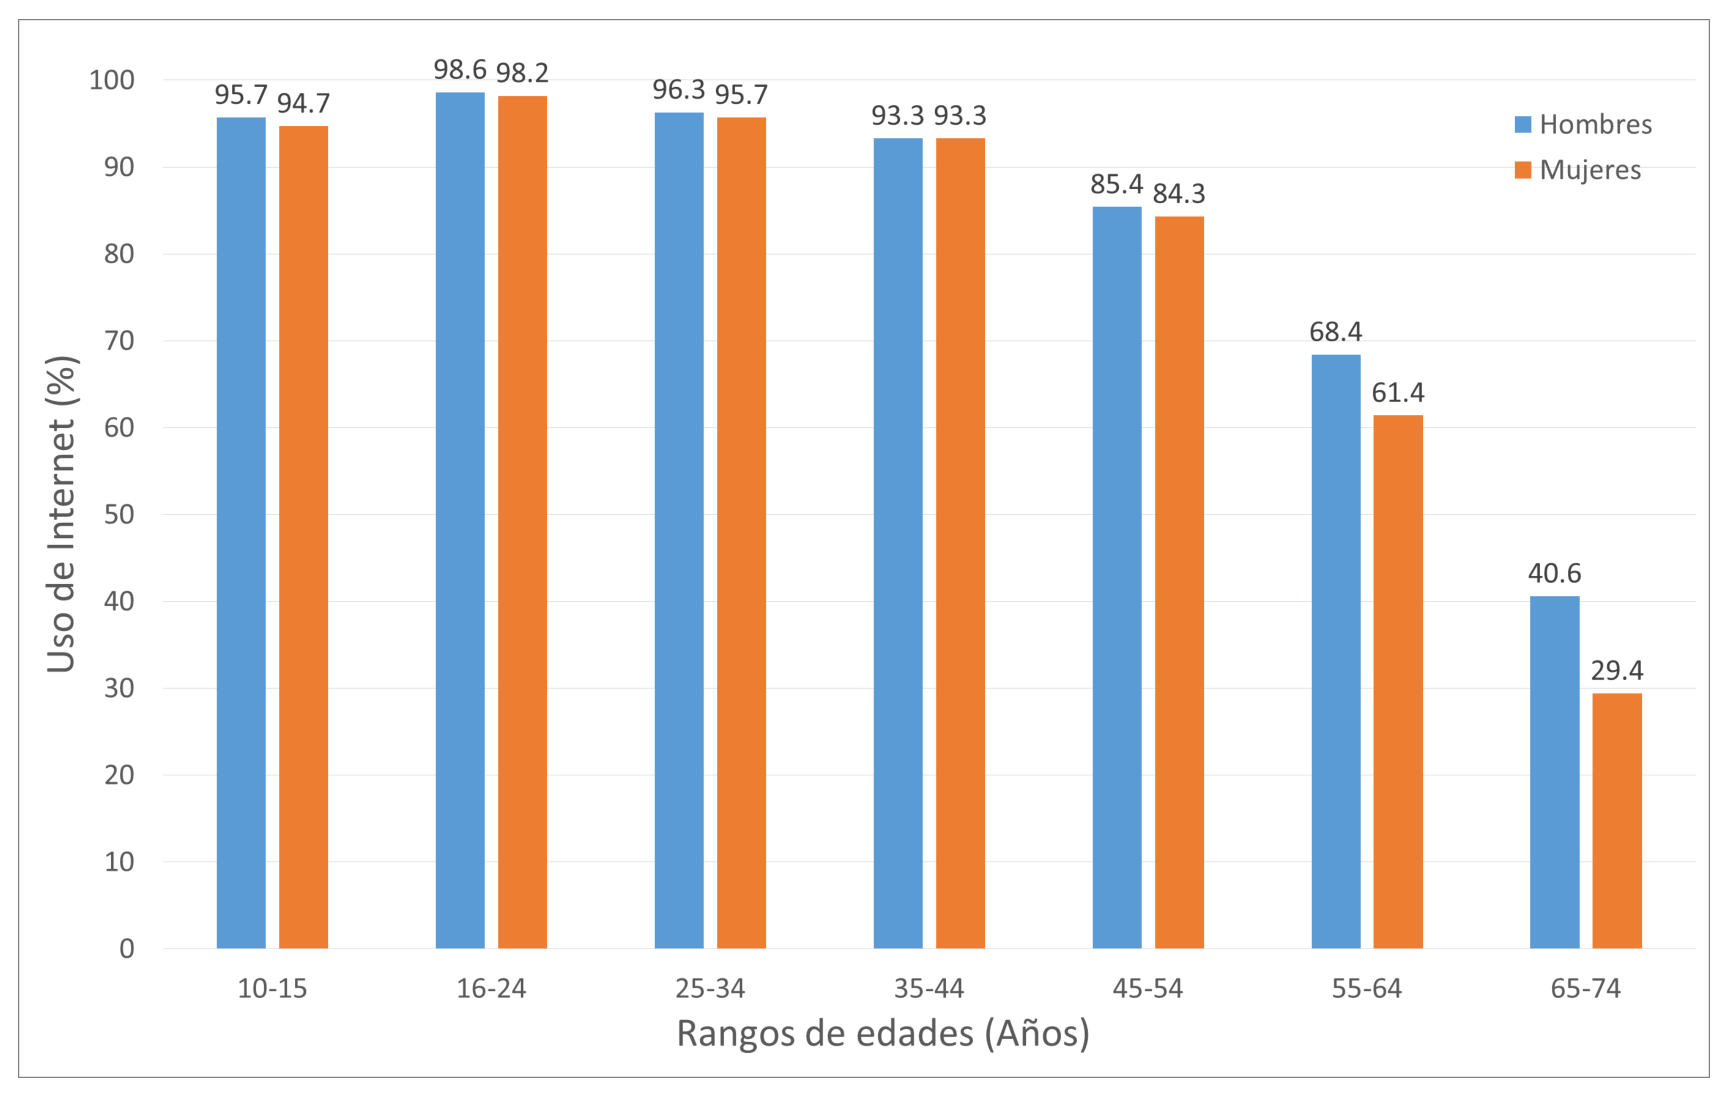
\includegraphics[scale=0.5]{internet_ages.eps}
        \caption{Uso de internet en función de la edad}
        \label{fig:internet_ages}
\end{figure}

Actualmente, es común que los menores de edad dispongan de dispositivos móviles desde los cuales puedan acceder a Internet, sin embargo, esto conlleva a que debido a su inmadurez y falta de experiencia, terminen pasando más tiempo del recomendado frente a una pantalla, sin dedicarle el tiempo necesario a sus obligaciones en casa, desatendiendo sus estudios o directamente perdiendo la comunicación con los seres que lo rodean. Además, es muy importante tener en cuenta que Internet no solo está lleno de ventajas, sino también de peligros. Un medio con tanto alcance y facilidad para las comunicaciones, hace que lograr el anonimato no sea un problema para cualquier persona con un mínimo de conocimientos técnicos, por lo que no es extremadamente raro escuchar casos donde un menor ha sido víctima de acoso, intimidación o incluso secuestro.

Para evitar estos problemas, los padres deben educar a los menores con buenas prácticas de navegación. Controlar la información que dan en Internet, las personas que conocen y el tiempo que pasan ``en línea" es fundamental para evitar malas experiencias.

No obstante, muchas de las herramientas disponibles para este control educativo precisan de conocimientos relativamente avanzados de informática y redes, como conocer las direcciones MAC de los dispositivos conectados, navegar por menús web con terminología demasiado técnica o aplicar y habilitar filtros basados en campos y criterios en su mayor parte desconocidos, por citar sólo alguno de ellos, cuando la mayoría de las veces lo único que se pretende es habilitar o no la conexión a Internet a un dispositivo concreto. Además, una buena parte de las herramientas que permiten este tipo de control sólo son accesibles en entorno web, accesible a su vez sólo desde el interior de los locales donde se encuentra la pasarela de acceso a Internet (conocida popularmente con el término de ``Router'').

Por tanto, la disponibilidad de una aplicación adaptada para dispositivos móviles, accesible desde cualquier punto de Internet y que permita la realización de las funciones básicas de control de una red Wi-Fi doméstica de forma sencilla y transparente y en un lenguaje adaptado al perfil de un usuario básico (como habilitar la conexión Wifi a un móvil A, deshabilitar el acceso a la consola de juegos o al ordenador de la habitación de los niños), puede ser de gran utilidad y disponer de una gran demanda.

En este trabajo se ha creado una aplicación para dispositivos móviles Android que cubre esta demanda para un tipo de pasarela doméstica concreta, aunque el modelo puede ser exportado para cualquier otra que tenga posibilidad de desarrollo de servicios software dentro del sistema operativo que la ejecuta. Particularmente la tecnología de acceso a Internet controlada es la tecnología 802.11, más conocida como Wifi, aplicable en el ámbito doméstico donde las pasarelas cuentan con esa tecnología (la inmensa mayoría) y los dispositivos se conectan a Internet a través de ella.

A pesar de que la parte visible del sistema es sólo la aplicación Android, deliberadamente sencilla, el sistema consta de un servicio instalado en la pasarela que recibe las instrucciones de la aplicación Android y ejecuta las acciones pertinentes en la pasarela de filtrado o habilitación/deshabilitación de accesos.

\cleardoublepage \section{Objetivos} \label{sec:obj}
% presentar o problema que se vai tratar, incluír o obxectivo principal e os
% específicos, de ser o caso, do traballo presentado, indicando o alcance para cada un deles.
    Se presenta en la figura \ref{fig:red_soho} un esquema general de una red doméstica donde se incluye la terminología empleada.

    \begin{figure}[h!][hp]
    \centering
        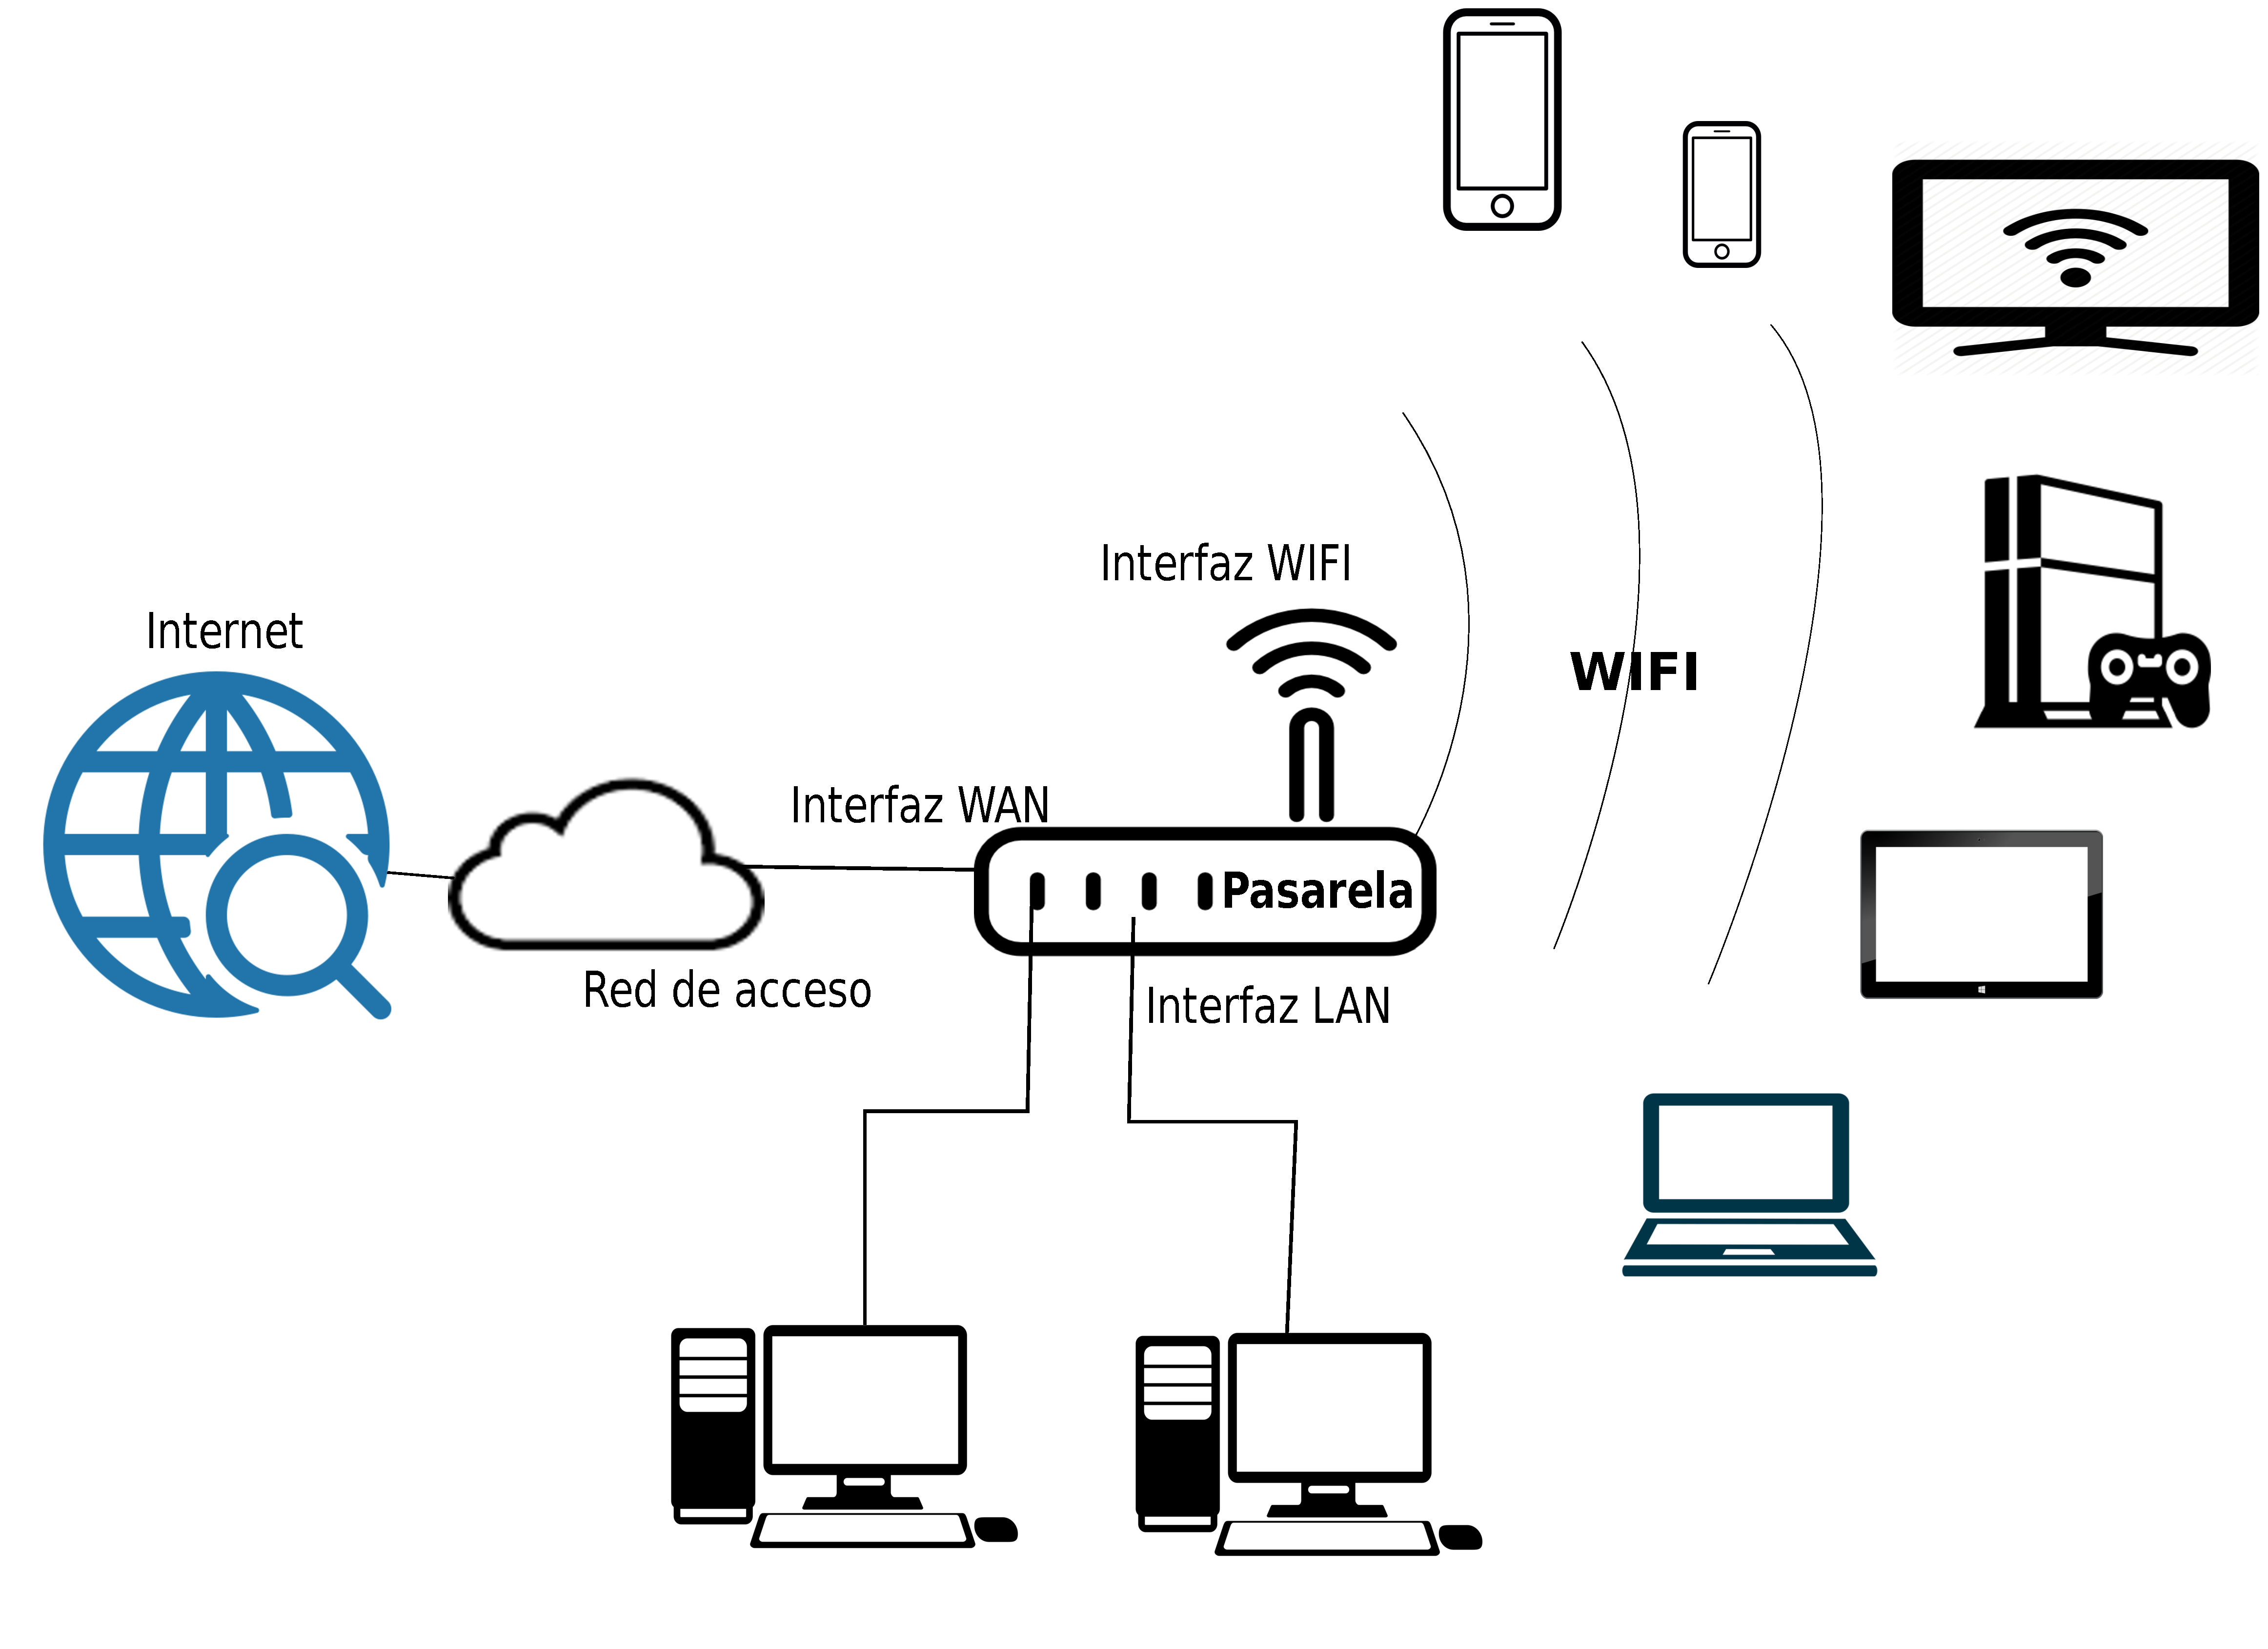
\includegraphics[scale=0.2]{soho_network.eps}
        \caption{Topología de una red doméstica}
        \label{fig:red_soho}
    \end{figure}

    Básicamente una red doméstica de acceso a Internet consta de un dispositivo central (comúnmente conocido como ``Router'') pero con funcionalidades mas amplias y adaptadas a este tipo de redes, y a su vez con menos capacidad de proceso en general que un Router profesional. En adelante a este dispositivo se le llamará ``Pasarela'' o ``Gateway'' (en su terminología en inglés). Además de la Pasarela, una red doméstica puede contar con una instalación básica de cableado horizontal tipo par-trenzado de diferentes categorías, y elementos repetidores como conmutadores o incluso elementos repetidores de radio-frecuencia.

    La pasarela dispone fundamentalmente de tres interfaces (aunque la mayoría añade una nueva interfaz para la conexión cableada de periféricos a través del bus USB): 

    \begin{description}
        \item[\underline{Interfaz WAN:}] Es la interfaz de acceso a Internet, llamada técnicamente \textit{interfaz a la red de acceso}. Esta interfaz puede tener un conector coaxial o de fibra óptica, aunque en muchas ocasiones utiliza también un conector RJ45 diferenciado de las interfaces LAN mediante un indicador, color o por estar en una posición diferente. En el caso de que la red de acceso sea inalámbrica, la interfaz WAN se muestra mediante una antena, mas o menos diferenciada de otras que pueda contener la Pasarela. La configuración de esta interfaz suele realizarse remotamente desde el operador de la red de acceso, ya que el correcto funcionamiento de la misma es su responsabilidad. El otro extremo del medio de transmisión conectado a ella (cable, fibra óptica o radio-frecuencia) se encuentra en las dependencias del operador. Por ello, se puede decir que la interfaz WAN es el enlace a Internet de la red doméstica.
        \item[\underline{Interfaz LAN:}] Es una interfaz (en su inmensa mayoría con conector RJ45) que permite la conexión de equipos domésticos cableados a la Pasarela. Aunque físicamente aparezcan varios conectores RJ45 para esta labor, a nivel lógico la interfaz LAN es sólo una. A los diferentes conectores de la interfaz LAN se les llama ``puertos'' y la conexión entre ellos se dice que es conmutada. El hecho de que lógicamente sólo sea una interfaz implica que no se pueden bloquear o desbloquear puertos individuales; cualquier operación lógica que se realice sobre la LAN, tendrá efectos sobre todos los puertos de la misma.
        \item[\underline{Interfaz WIFI:}] La interfaz WIFI es una antena, exterior o interior. Aunque suele estar internamente conectada a la interfaz LAN (puente LAN-WIFI) tiene características especiales, pues suele habilitar a un segmento de red diferenciado de la interfaz LAN. El segmento al que da acceso es inalámbrico por tecnología 802.11 b/g/n, llamada popularmente Wifi (de ahí el nombre de la interfaz). Los dispositivos a los que da acceso esta interfaz son dispositivos inalámbricos, como ordenadores portátiles, consolas, teléfonos móviles o tablets. Últimamente también se pueden encontrar dispositivos domóticos con interfaz WIFI compatible. La habilitación del acceso a Internet a través de esta interfaz es altamente configurable, pudiéndose individualizar los accesos de los dispositivos por su dirección MAC u otras características. El proceso de configuración tanto de la interfaz WIFI como de los dispositivos que se pueden conectar a ella será el objetivo principal de este proyecto.
    \end{description}

    Teniendo en cuenta todo lo mencionado anteriormente, se decide realizar un estudio de necesidades generales analizando las características de los routers domésticos. Con los resultados obtenidos se debe crear un sistema capaz de controlar redes Wi-Fi similares a las que comunmente pueden ser encontradas en los hogares. De esta forma  los padres pueden limitar el uso de Internet a los menores de forma sencilla y sin necesitar conocimientos avanzados de informática.
    \begin{enumerate}
        \item \textbf{\underline{Control desde dispositivos móviles}} \\
            El sistema debe ser capaz de ser controlado desde dispositivos móviles con los que se tenga accesso al router, el control deberá ser posible desde el exterior, mediante la interfaz WAN y desde dentro de la propia red doméstica, ya sea mediante la interfaz LAN, o la prropia interfaz Wi-Fi.
        
        \item \textbf{\underline{Encender y apagar red Wi-Fi}} \\
            Se debe implementar un mecanismo de control que permita encender o apagar la red Wi-Fi desde el dispositivo cliente de forma sencilla e inmediata.

        \item \textbf{\underline{Filtro MAC}} \\
            Se busca implementar la gestión de un filtro MAC de tres estados, los cuales permitan gestionar los dispositivos a la red Wi-Fi, los diferentes estados con los que debe contar el filtro son:
            \begin{itemize}
                \item \textbf{Desactivado:} Permite que todos los dispositivos puedan tener acceso a la red Wi-Fi.
                \item \textbf{Permitir:} Solamente permite que sean conectados a la red Wi-Fi los dispositivos explícitamente especificados. 
                \item \textbf{Denegar:} Permite el acceso a la red Wi-Fi a todos los dispositivos excepto a los que sean explícitamente especificados.
            \end{itemize}
        \item \textbf{\underline{Seguridad contra dispositivos no autorizados}} \\
            Aplicar un mecanismo de seguridad que elimine la posibilidad de que se pueda tomar el control del router desde un dispositivo móvil no autorizado.
        \item \textbf{\underline{Seguridad contra la réplica de paquetes}} \\
            Aplicar un mecanismo de seguridad capaz de impedir la réplica de paquetes de red que permitan cambiar configuraciones en el router de forma desautorizada.
        \item \textbf{\underline{Soporte para idiomas}} \\
            La aplicación cliente debe ser multilingüe, con soporte para los idiomas español e inglés, donde este último sea el idioma configurado por defecto al ser instalada.
    \end{enumerate}


\cleardoublepage \section{Resumen de la solución propuesta} \label{sec:sol}
% indicarase a solución aportada para o problema
% presentado. Deberase incluír aquí a metodoloxía empregada.
    Tras realizar un análisis de los componentes con los que comunmente se cuenta en entornos domésticos, se ha concluido que no es posible crear una solución estándar para los diferentes proveedores de servicios de Internet, por tanto, se plantea la realización de un sistema de control parental sobre accesos Wi-Fi en un router con OpenWRT, un sistema operativo compatible con un gran número de los routers actuales del mercado y adaptable a la mayoría de los existentes. 
    
    Se creará una aplicación sobre Android para el control de los dispositivos conectados a la red Wi-Fi doméstica, y una servicio que se ejecute como demonio en el router, donde se recibirán conexiones desde la aplicación con la configuración a establecer. La conexión se realizará mediante paquetes UDP, evitando así el establecimiento de conexión y ganando en velocidad.

    La funcionalidades de la aplicación se desarrollarán utilizando los propios mecanismos proporcionados por OpenWRT para el control de sus sistemas. El apagado/encendido de la red Wi-Fi se realizará a través del comando \textit{wifi} con los argumentos necesarios en cada caso, mientras que la gestión del control de accesos se llevará a cabo mediante los archivos de configuración de ubicados en \textit{/etc/config}.

    Para llevar a cabo la creación de este sistema, inicialmente se valoró el uso de una metodología de desarrollo en cascada, sin embargo, tras una nueva aproximación al problema, se llegó a la conclusión de que esta no era la solución más acertada debido a que el sistema se basa en un entorno de red, además se necesita realizar compilación cruzada utilizando un SDK específico, el cual cuenta con sus propias librerías, y la documentación de la que se dispone puede estar incompleta, desactualizada o errónea en su totalidad. Esto lleva como consecuencia que se necesite realizar pruebas de envíos de paquetes constantemente, y que, debido a la diferencia de librerías, se requiera realizar cambios en el código que se plantee inicialmente. También es necesario que el sistema ocupe el menor espacio posible, ya que el espacio de almacenamiento en routers suele ser limitado, lo que llevará a que el codigo deba ser refactorizado constantemente.
    
    Tras el análisis anterior, se ha concluído que lo más adecuado sería el uso de un método ágil de desarrollo, en concreto \textit{SCRUM}, que está más enfocado a la administración del desarrollo iterativo. \textit{SCRUM} consta de tres fases:
    
    \begin{itemize}
        \item Planificación de un \textit{boceto}, donde se establecen los objetivos generales del proyecto y el diseño de la arquitectura del software.
        \item Una serie de ciclos \textit{sprint}, donde cada ciclo desarrolla un incremento del sistema.
        \item \textit{Cierre} del proyecto, fase en la cual se completa la documentación requerida como ayudas y manuales de usuario.
    \end{itemize}

    \textit{SCRUM} permite que el producto se desglose en piezas comprensibles de forma individual y que son desarrolladas de forma iterativa, recibiendo retroalimentación del usuario con cada entrega y realizando cambios en consecuencia. Para llevar a cabo el desarrollo utilizando este método, es necesario ocupar los roles imprescindibles para su funcionamiento.

    \begin{itemize}
        \item \textbf{Equipo de desarrollo:} Equipo responsable de llevar a cabo el desarrollo del sistema. Este rol estará compuesto únicamente por el alumno.
        \item \textbf{Cliente:} Encargado de defininir los requisitos, utilizar las versiones resultantes de cada \textit{sprint} y aportar retroalimentación para la mejora del sistema. Este rol será llevado a cabo por el tutor del TFG.
        \item \textbf{Maestro de SCRUM:} Encargado de rastrear el trabajo que queda por hacer, tomar desiciones, medir el avance en función de la planificación inicial y mantener la comunicación con el cliente. Este rol será adoptado por el alumno.
    \end{itemize}

\cleardoublepage \section{Planificación y seguimiento} \label{sec:plan}
% deberase incluír un diagrama de Gantt que amose tanto
% a planificación do traballo, coa súa distribución de fases e tarefas, e a súa comparación cos
% datos reais obtidos tras o desenvolvemento do traballo.
    Como se expone en el apartado \ref{sec:sol}, la metodología de desarrollo empleada para llevar a cabo en este proyecto es \textit{SCRUM}. Por tanto, una vez conocida la solución a realizar, se realiza una planificación que incluye todo el trabajo necesario para el desarrollo del sistema dividiéndolo en sprints, que a su vez están compuestos por subtareas.

    \subsection{Planificación inicial}
        \subsubsection{Diagrama de fases y tareas}
        Como se muestra en la \ref{tab:fases_planif} el desarrollo del sistema se llevará a cabo durante nueve fases, entre las cuales se incluyen cinco sprints de implementación y la elaboración de la documentación, que incluye la fase de cierre, fundamental en \textit{SCRUM}.

        \begin{table}[h!]             
                \centering                  
                    \resizebox{\textwidth}{!}{   
                        \begin{tabular}{|l|c|}
                            \hline
                            \textbf{Fase}  & \textbf{Estimación temporal} (Días) \\           
                            \hline
                            Investigación                                                       &   2    \\
                            Boceto                                                              &   2    \\
                            Compilación cruzada                                                 &   4    \\
                            Sprint 1: Implementaciónde la aplicación Android base               &   5    \\
                            Sprint 2: Implementación del servidor                               &   5    \\
                            Sprint 3: Implementación de sistemas de seguridad                   &   5    \\
                            Sprint 4: Implementación de la interfaz gráfica de la aplicación    &   10   \\
                            Sprint 5: Integración de sistemas                                   &   5    \\
                            Documentación                                                       &   52   \\
                            \hline
                        \end{tabular}
                    }
                \caption{Planificación de las fases}
                \label{tab:fases_planif}
            \end{table}

        En las imágenes \ref{fig:fases} y \ref{fig:fases_gantt} se puede apreciar la planificación de las nueve fases.

        \begin{figure}[h!]
            \centering
                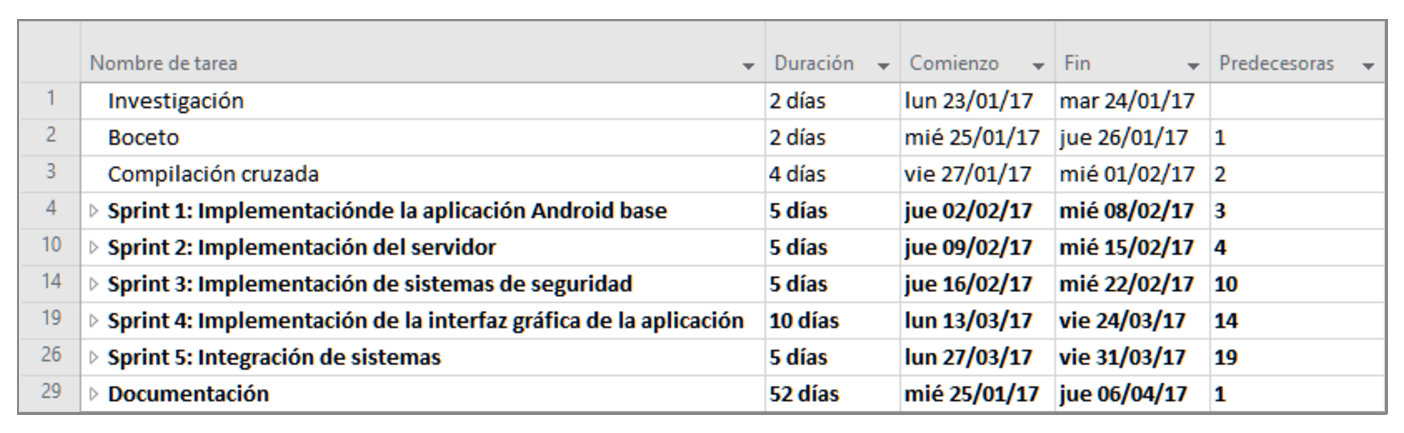
\includegraphics[scale=0.7]{fases.eps}
                \caption{Planificación de las fases del proyecto}
                \label{fig:fases}
        \end{figure}

        \begin{figure}[h!]
            \centering
                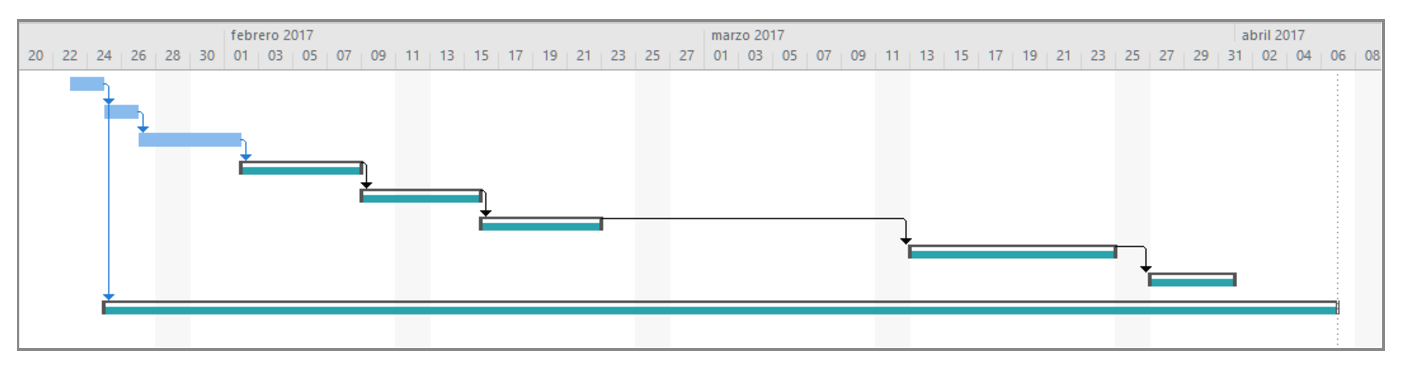
\includegraphics[scale=0.7]{fases_gantt.eps}
                \caption{Diagrama de Gantt de las fases}
                \label{fig:fases_gantt}
        \end{figure}

        Las figuras \ref{fig:tasks}, \ref{fig:tasks_gantt0} y \ref{fig:tasks_gantt1} muestran la planificación de las tareas del proyecto. Es importante destacar el intervalo de dieciocho días de la planificación donde se detienen las actividades, esto es debido a que el equipo de desarrollo no se encuentra disponible en este período.

        \begin{figure}[h!]
            \centering
                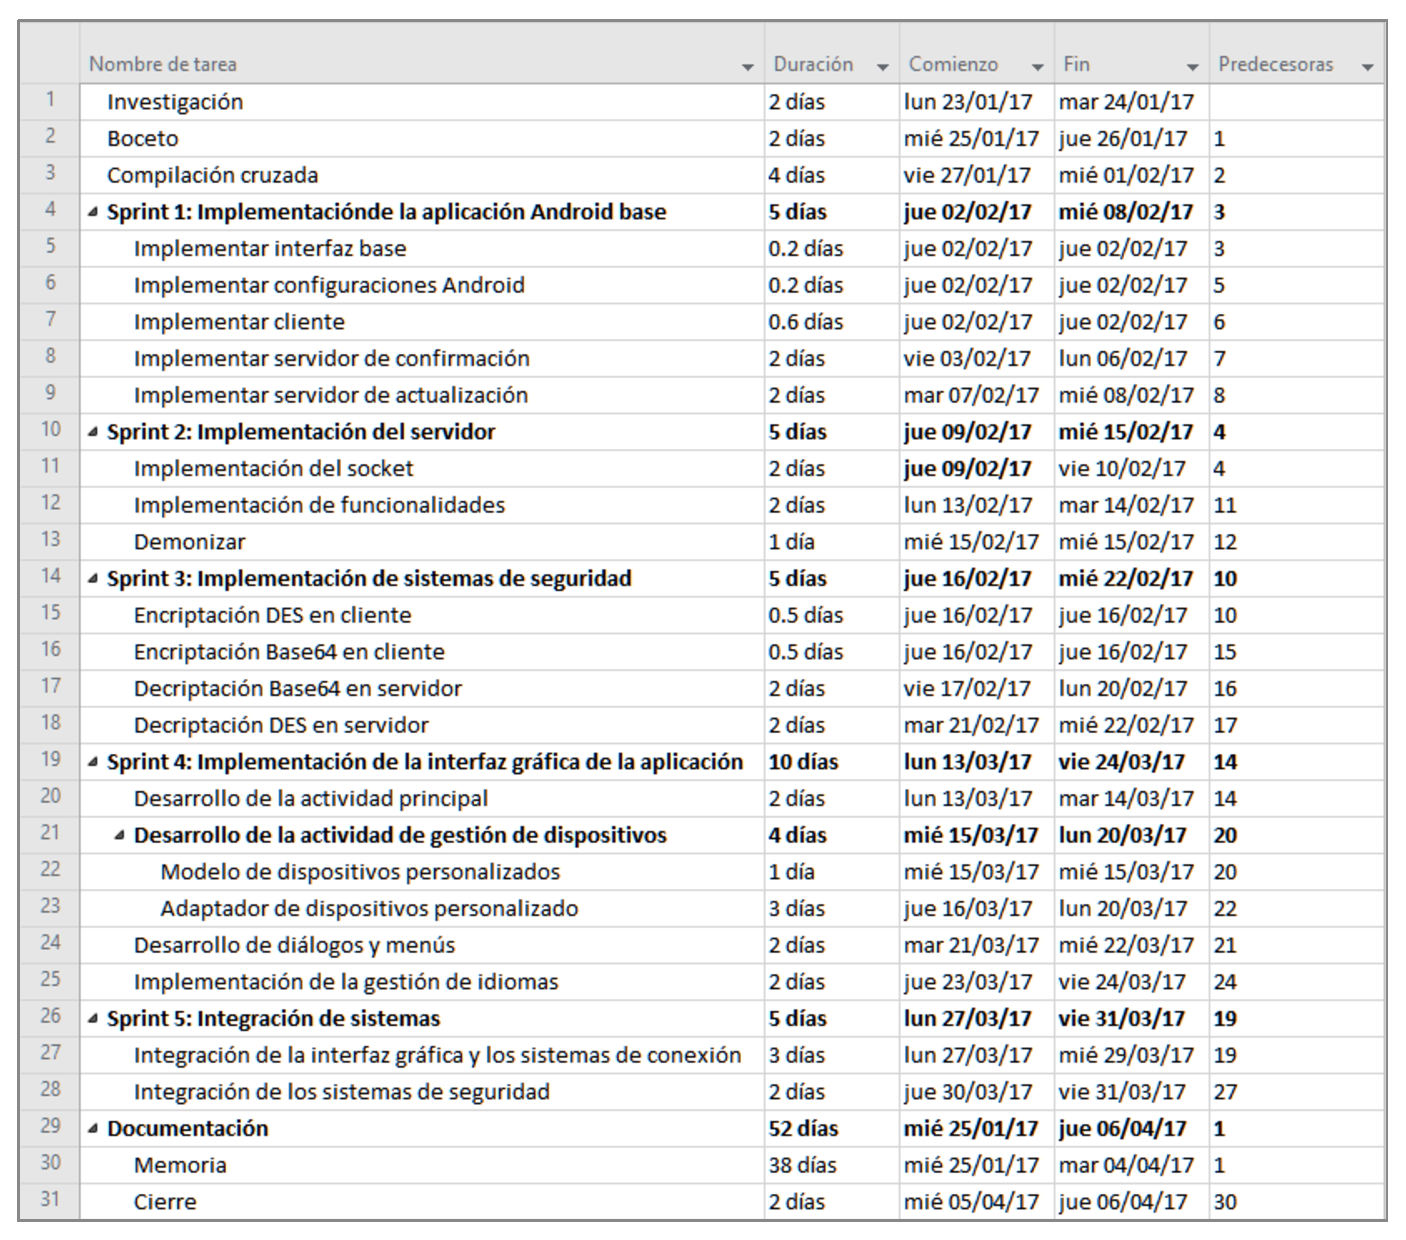
\includegraphics[scale=0.7]{tasks.eps}
                \caption{Planificación de las tareas del proyecto}
                \label{fig:tasks}
        \end{figure}

        \begin{figure}[h!]
            \centering
                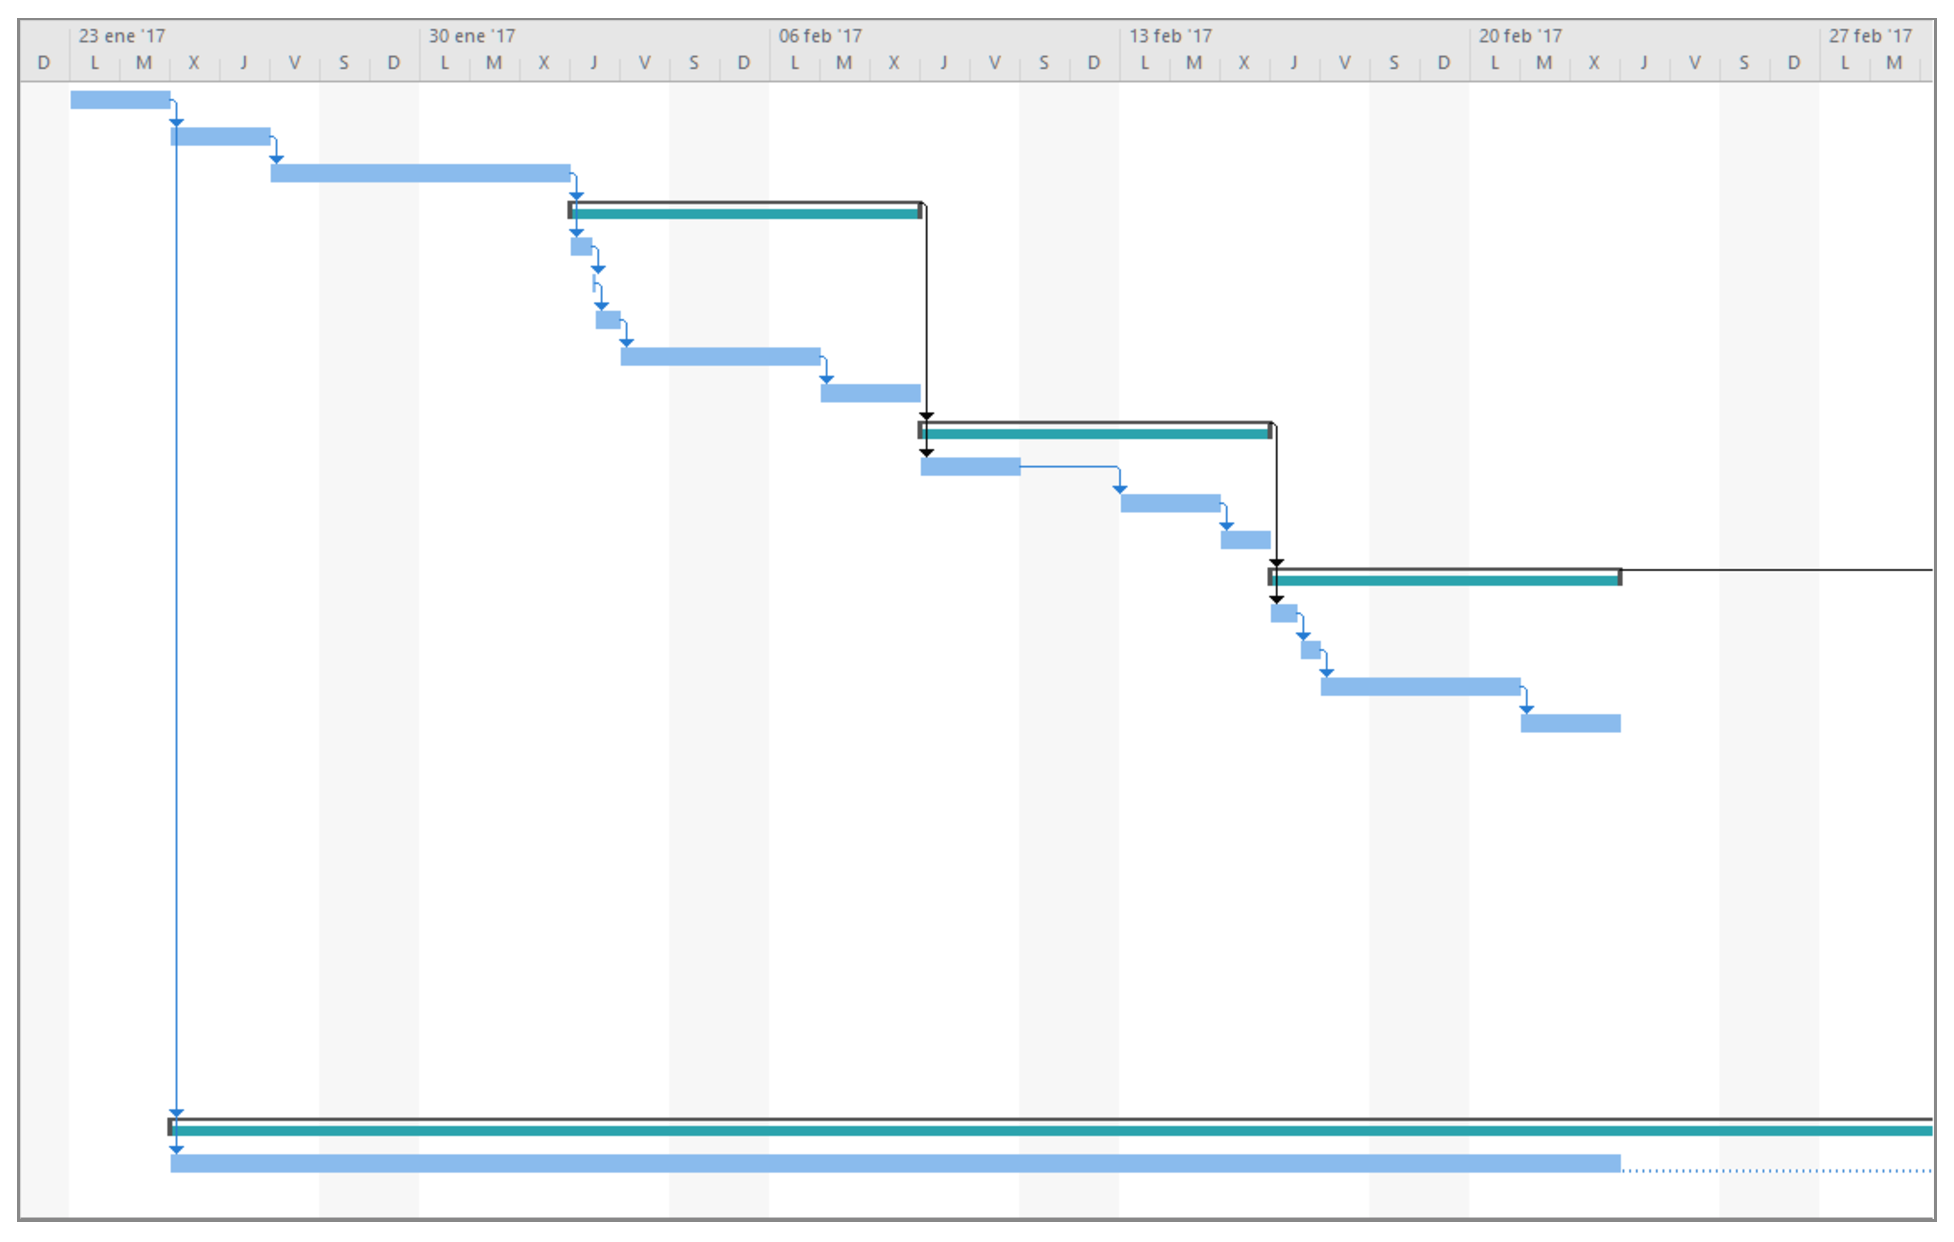
\includegraphics[scale=0.5]{tasks_gantt0.eps}
                \caption{Diagrama de Gantt de las tareas}
                \label{fig:tasks_gantt0}
        \end{figure}

        \begin{figure}[h!]
            \centering
                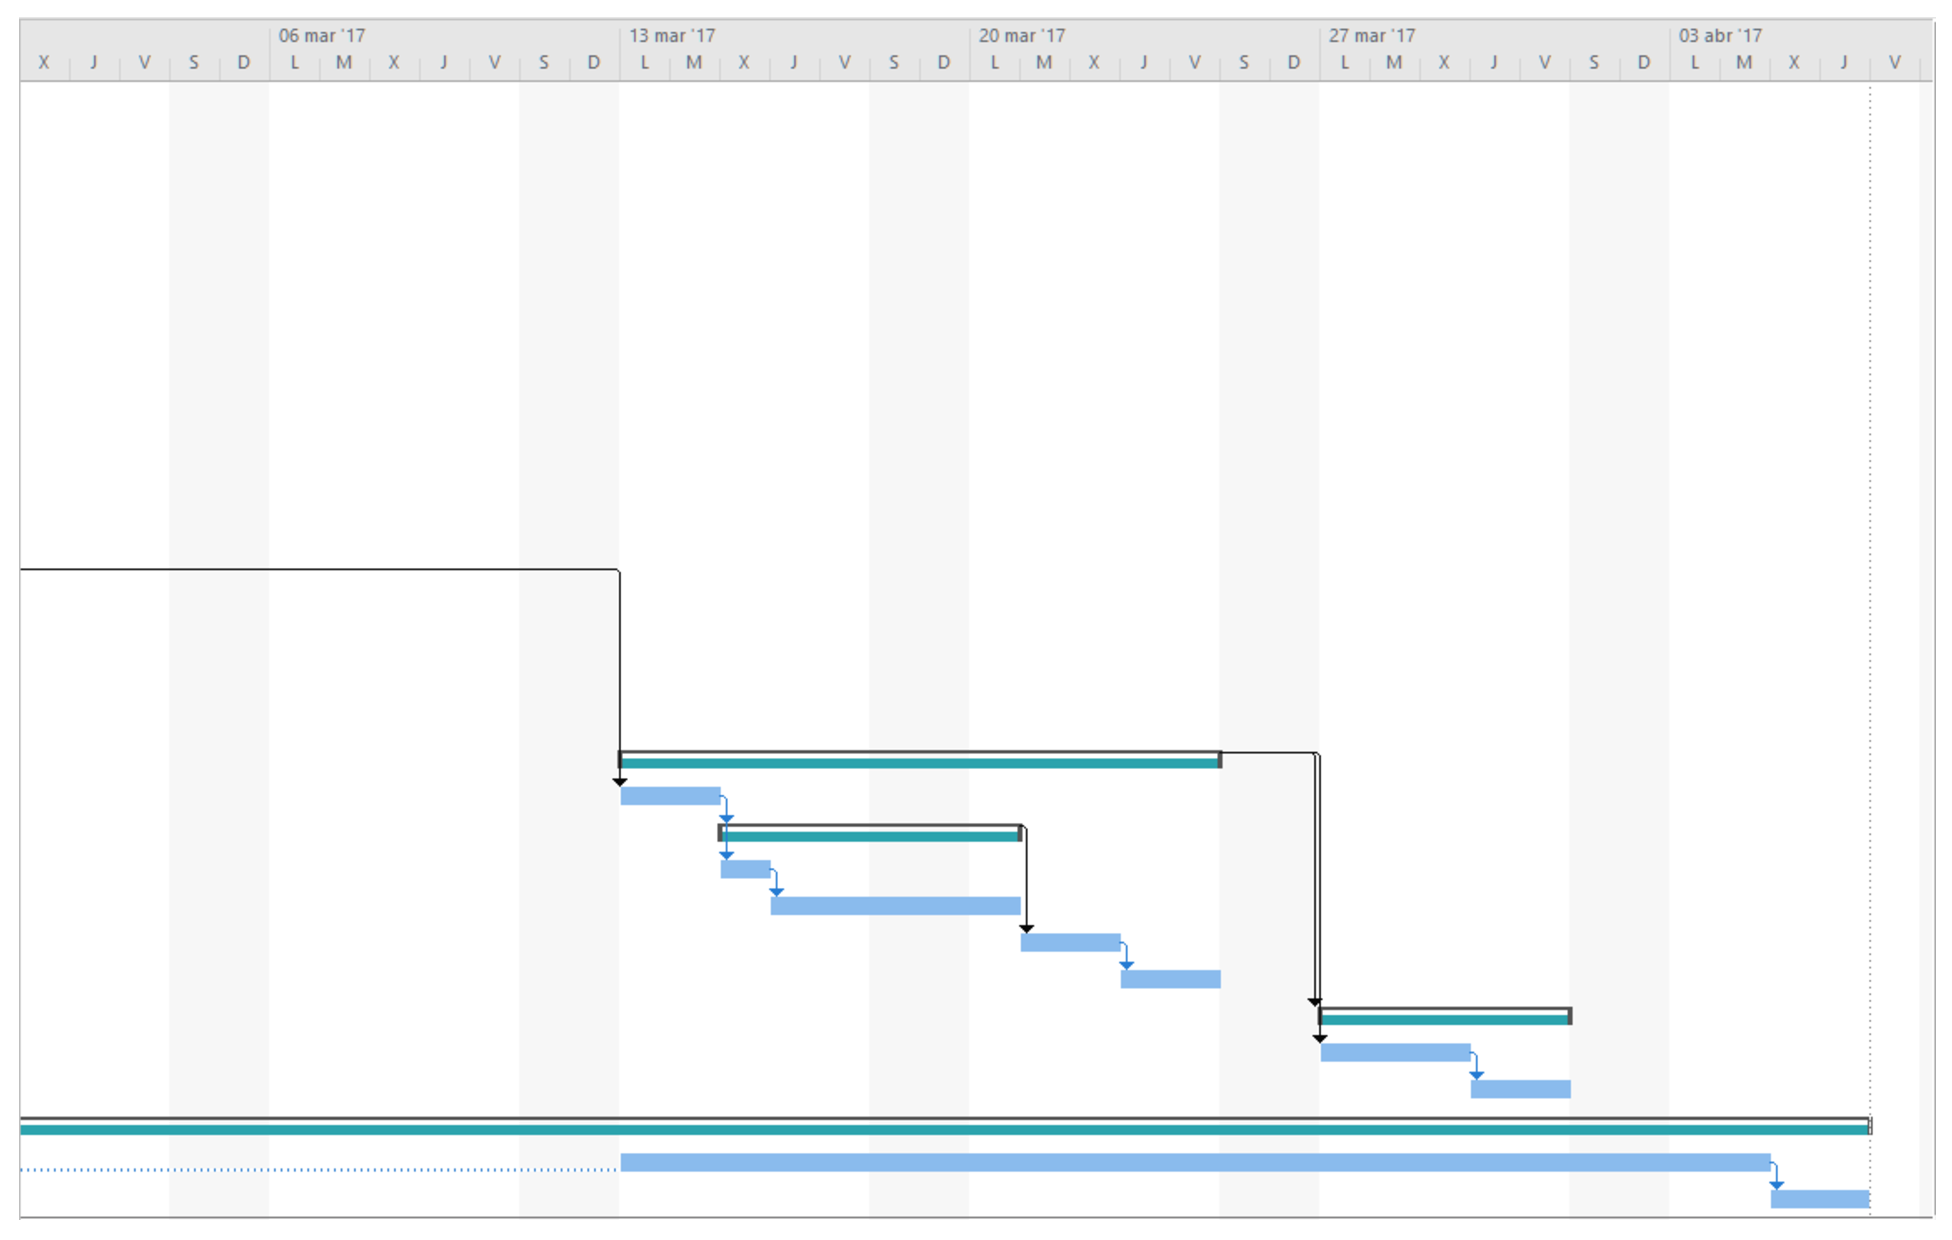
\includegraphics[scale=0.5]{tasks_gantt1.eps}
                \caption{Diagrama de Gantt de las tareas}
                \label{fig:tasks_gantt1}
        \end{figure}

    \subsection{Desviaciones de la planificación inicial}
        La planificación inicial es utilizada como una guía a seguir para la ejecución del proyecto, pero hay ocasiones en las que se hace imposible seguirla al pie de la letra. Esos momentos en los que la ejecución real difiere de la planificación son llamados ``Desviaciones'', y pueden estar causdas por múltiples motivos. Los principales son una planificación errónea o la aparición de imprevistos. Esto no es extraño que ocurra, por tanto, siempre se debe planificar teniendo en mente los problemas que puedan surgir durante el desarrollo del proyecto. El diagrama de Gantt con los datos reales obtenidos (figura \ref{fig:deviations_gantt}) y las principales desviaciones de este proyecto están detalladas a continuación.

        \paragraph{ Compilación cruzada}
        La primera desviación que surge en el proyecto aparece al intentar realizar la compilación cruzada. La documentación aportada por OpenWRT para realizar este proceso es muy escueta e incomprensible, y la información relacionada que pudo ser encontrada en Internet estaba desactualizadada desde 2007. Esto llevó a un largo proceso de prueba y error a partir de los antiguos procesos de compilación y la información obtenida de la página oficial, lo que provocó un retraso en todo el proyecto.

        \paragraph{ Implementación de sistemas de seguridad}
        La segunda y tercera desviación ocurren durante la implementación de sistemas de seguridad. Primeramente se decide utilizar la librería \textit{OpenSSL} para llevar a cabo el proceso de decriptación DES, sin embargo, siguiendo la documentación al pie de la letra y obteniendo información de Internet no se obtienen los resultados esperados. Debido a esto se decide utilizar una librería diferente que permita llevar a cabo el proceso especificado (\textit{libc}), pero tras el desarrollo de este fragmento del sistema y tras la validación de las primeras pruebas surge un problema al compilar, debido a que en OpenWRT \textit{libc} es sustituido por la versión reducida \textit{uClibc}, incompleta en este sentido, ya que solamente dispone de las cabeceras de los procesos necesarios para esta tarea, y no de su implementación. El problema es finalmente solucionado volviendo al punto de partida con \textit{OpenSSL}, y tras un proceso de prueba y error, se determina que existe un método cuyo resultado es diferente al indicado en la documentación oficial.

        La tercera desviación surge en el intento de añadir un mecanismo de seguridad que no estaba planificado inicialmente. Se realiza el intento de obtener la dirección MAC del dispositivo que envía peticiones al servidor en cada uno de los paquetes, con el objetivo implementar un mecanismo de control de accesos mediante el filtrado de los dispositivos autorizados. Tras varios intentos y pruebas, finalmente es descartado debido a que para realizarlo es necesario rehacer el socket desarrollado en el sprint anterior con un nuevo tipo, lo cual representa una desviación demasiado grande teniendo en cuenta las anteriores y las que aún pueden surgir a partir de este punto.

        \paragraph{ Implementación de la interfaz gráfica de la aplicación}
        La cuarta y última desviación surge con la gestión de \textit{listeners} de la interfaz gráfica durante el desarrollo de la actividad de gestión de dispositivos. Debido a que gran parte de la interfaz se realiza utilizando elementos personalizados muy diferentes de los que proporciona Android \cite{Color}, se hace difícil encontrar documentación para controlar situaciónes específicas. Los retos fundamentales, y los cuales toman una mayor cantidad de tiempo al inicialmente planificado son la vuelta atrás de la interfaz gráfica en caso de fallo, sin que sea lanzada una nueva ejecución del método; y la gestión de \textit{listeners} en los diálogos que permitan rotar la pantalla sin obtener resultados inesperados.
        
        \begin{figure}[h!]
            \centering
                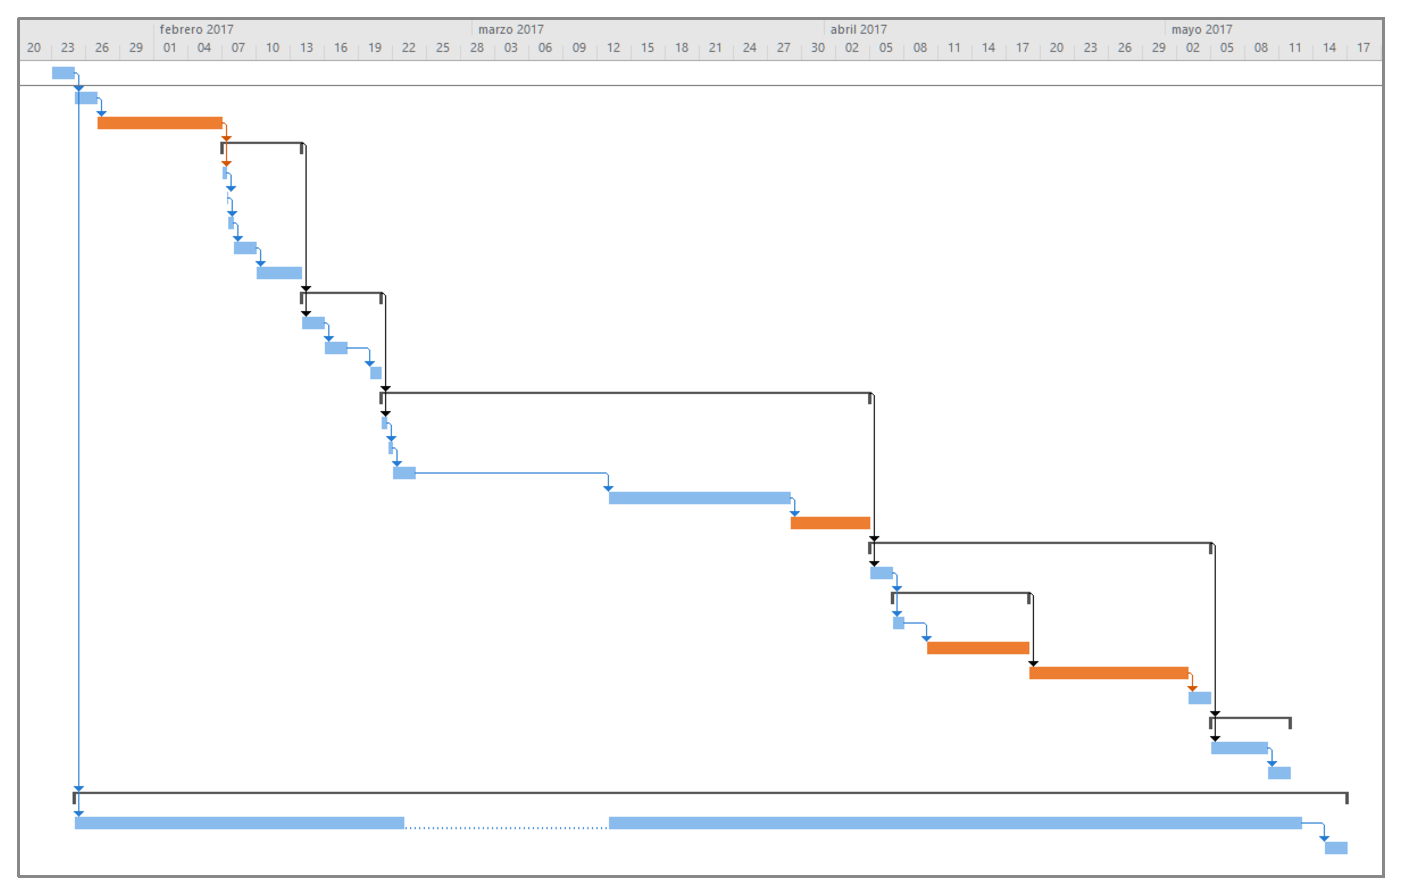
\includegraphics[scale=0.7]{deviations_gantt.eps}
                \caption{Diagrama de Gantt de las desviaciones}
                \label{fig:deviations_gantt}
        \end{figure}

        La arquitectura del servidor 

\cleardoublepage \section{Arquitectura y tecnologías} \label{sec:arq}
% explicarase a arquitectura empregada para alcanzar os obxectivos propostos.

    \subsection{Arquitectura del sistema}

        La arquitectura general del sistema está basada en el modelo \textit{Cliente-Servidor} de dos capas, la cual se define como un servicio o conjuntos de servicios a los que acceden y usan clientes. En este caso la aplicación móvil Android es la que realiza la función de cliente, enviando mensajes de control al router OpenWRT servidor, que se mantiene a la espera de mensajes para cambiar la configuración de la red de acuerdo lo que le sea indicado.

        Es importante destacar que el modelo utilizado es un modelo de \textit{cliente grueso}, ya que es el que lleva prácticamente toda la carga de procesamiento del sistema, este gestiona tanto el almacenamiento de configuraciones como el de dispositivos, además de los sistemas de confirmación. El servidor solamente es consultado desde el cliente para modificar archivos de configuración.

        \subsubsection{Componentes del sistema}
            En este apartado se detallan las diferentes partes que componen el sistema, así como la forma en la que se comunican entre ellos. En la figura \ref{fig:system_diagram} se muestra un diagrama de la arquitectura utilizada con los principales componentes del sistema.

            \begin{figure}[h!]
            \centering
                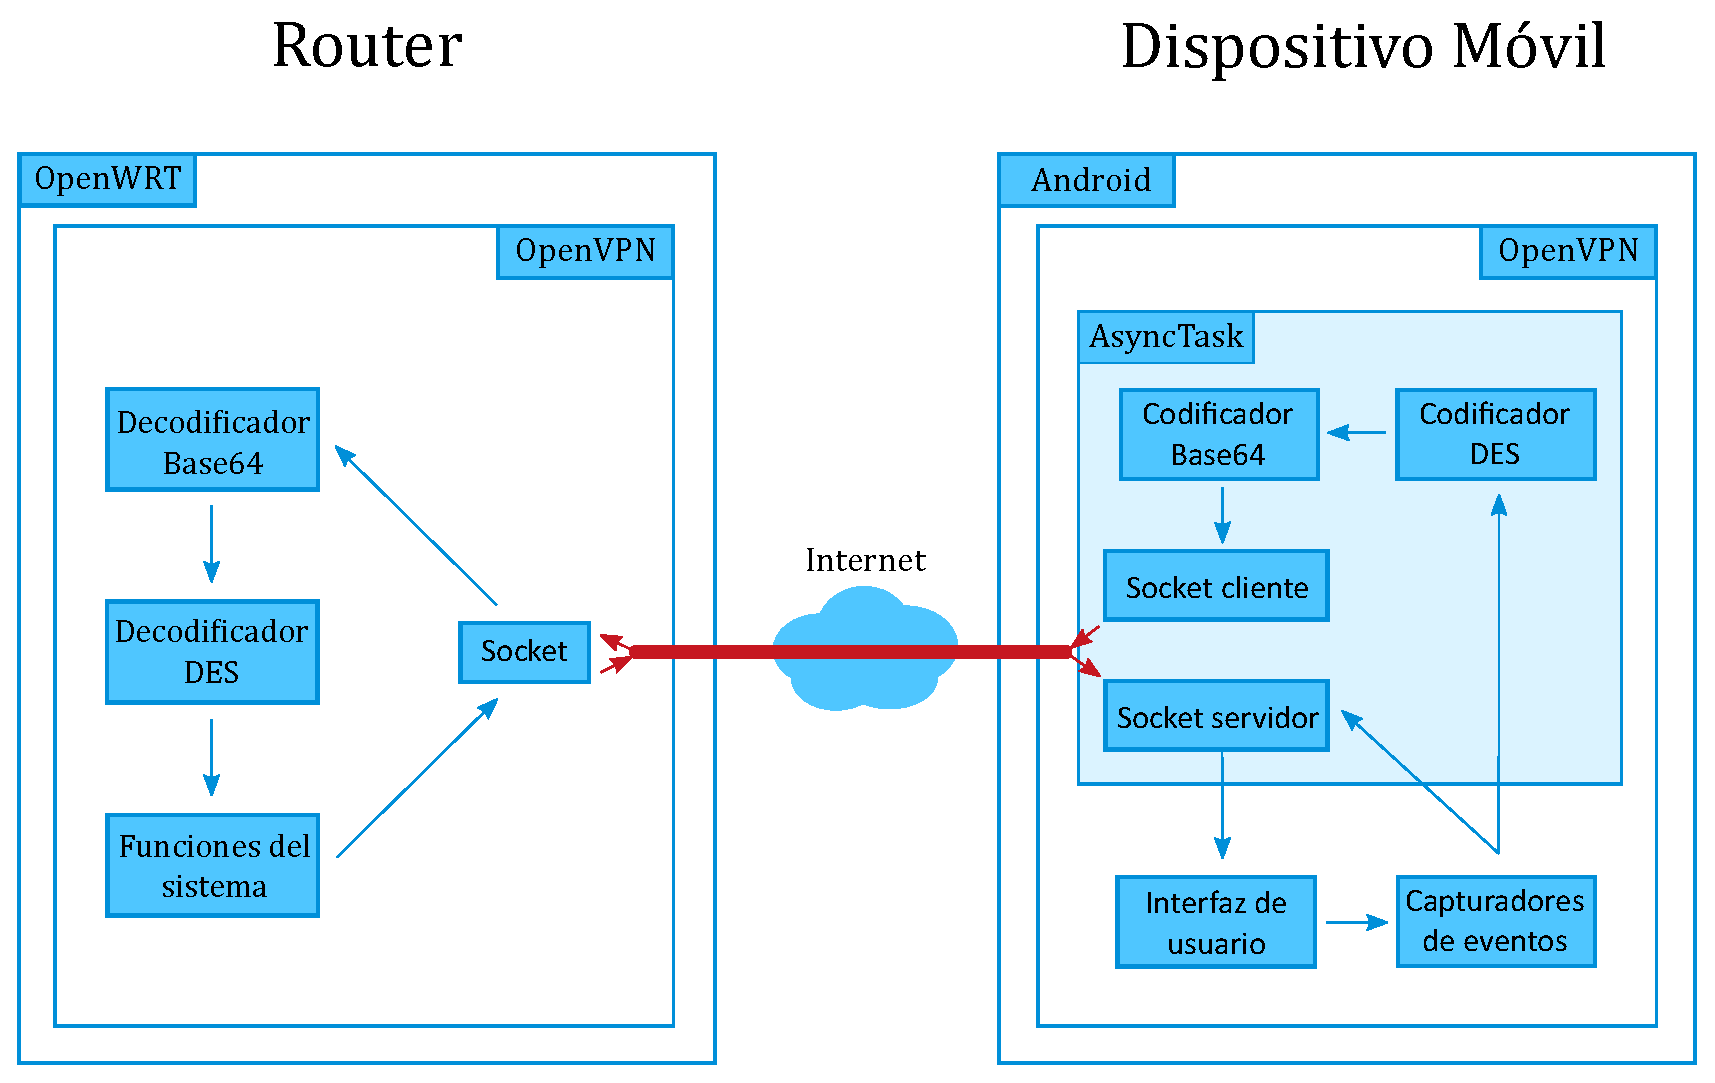
\includegraphics[scale=0.5]{system_diagram.eps}
                \caption{Diagrama de la arquitectura del sistema}
                \label{fig:system_diagram}
            \end{figure}

            \paragraph{ Servidor}
            El servidor es el encargado de recibir todas las peticiones desde el cliente y modificar los archivos de configuración de acuerdo a los parámetros de control que le hayan sido enviados. Al ser desarrollado en C no está compuesto por clases, sino por métodos que son interpretados como componentes, donde cada uno realiza una función específica. En la figura \ref{fig:server_diagram} se puede ver la estructura del servidor.

            \begin{figure}[h!]
            \centering
                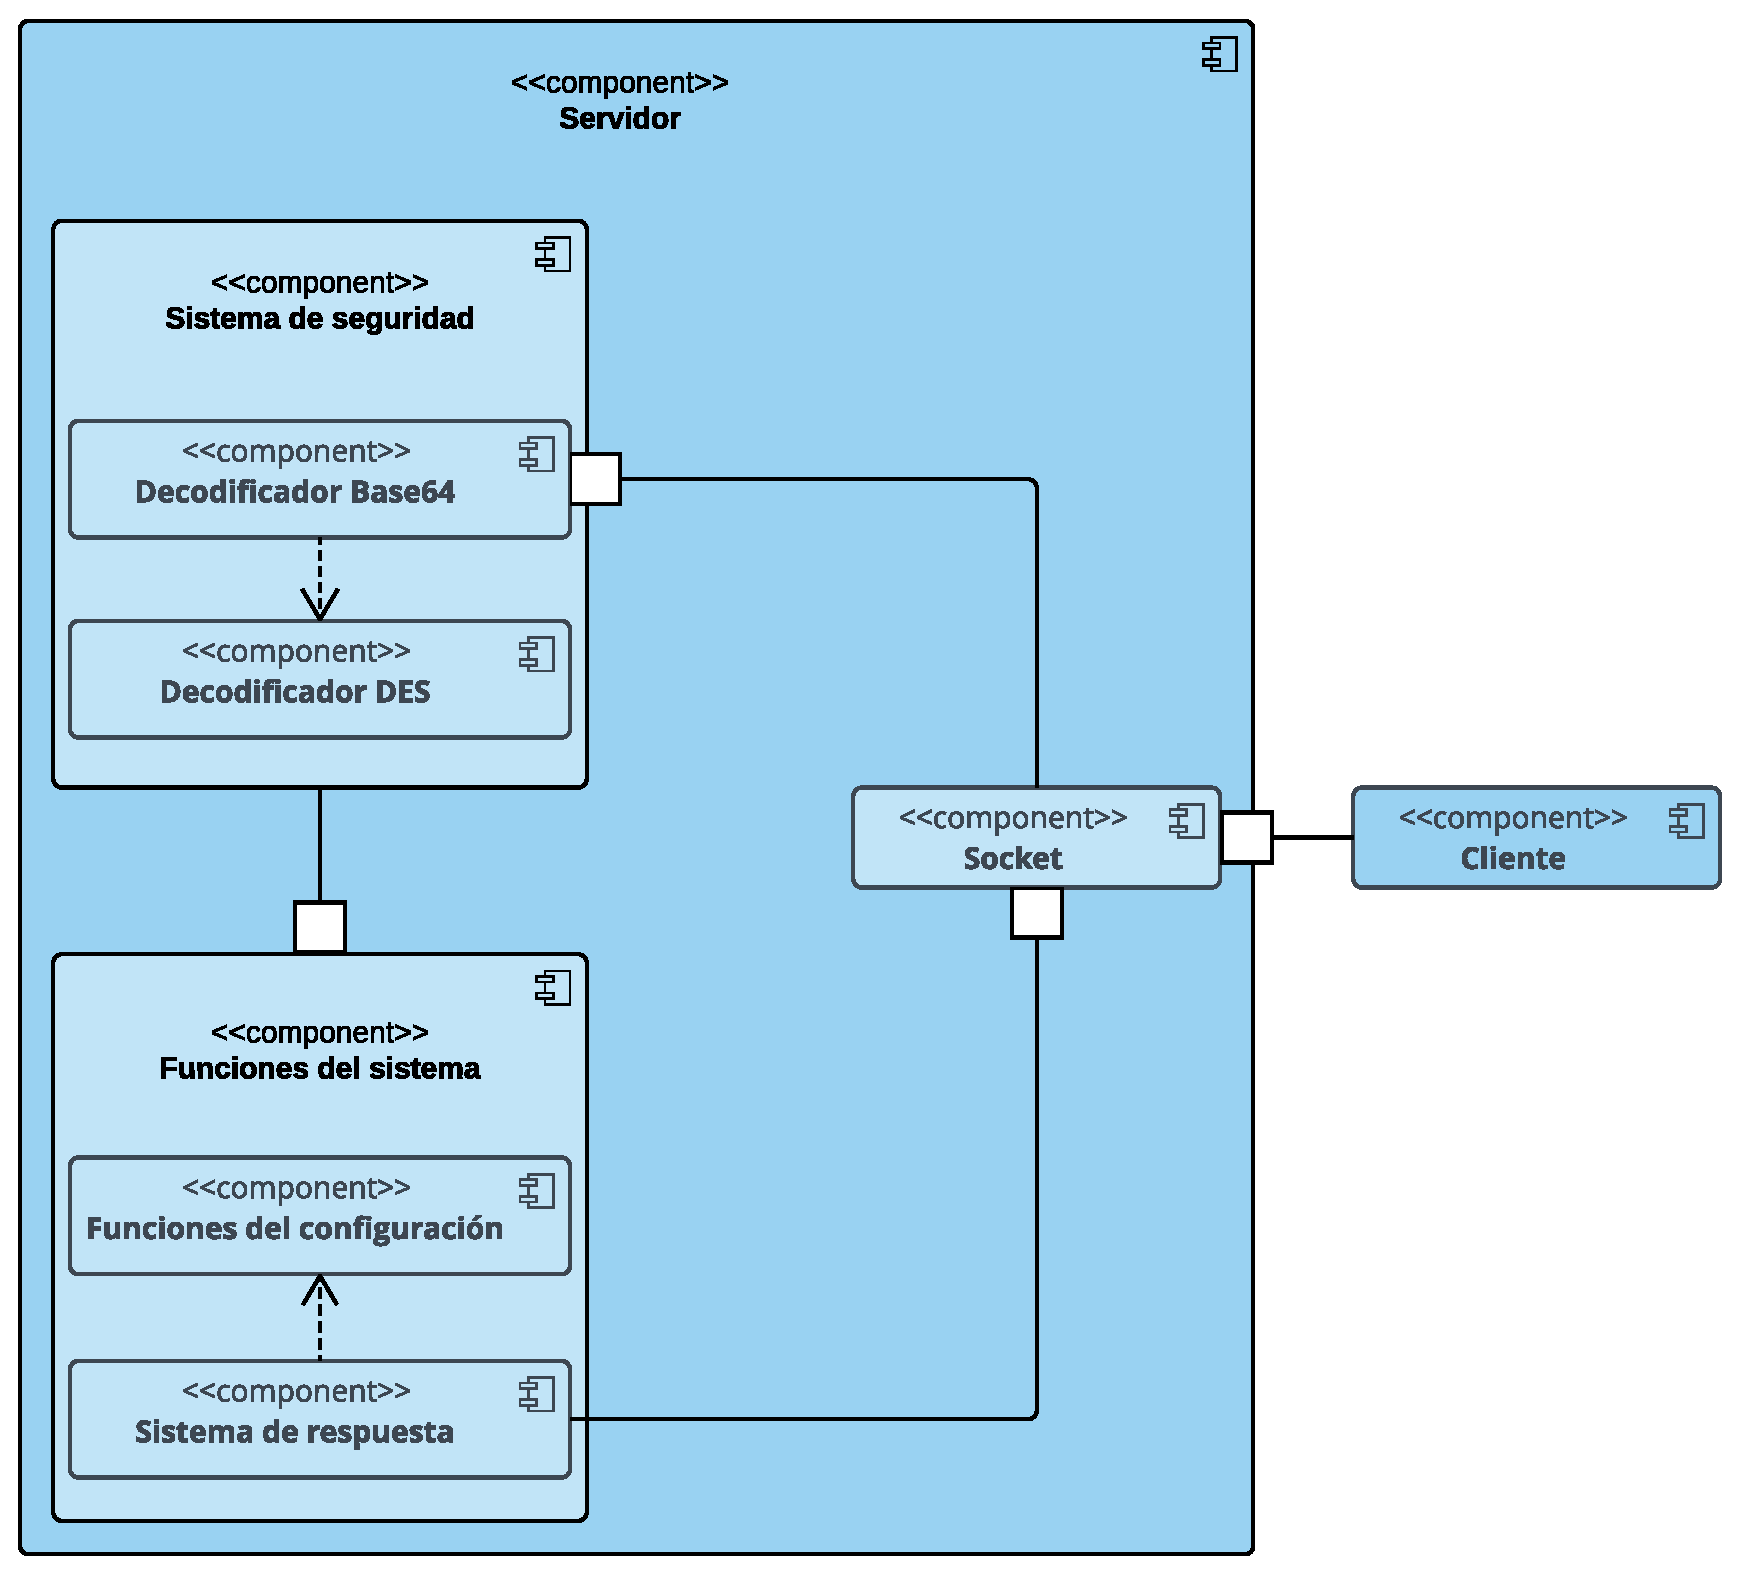
\includegraphics[scale=0.4]{server_diagram.eps}
                \caption{Diagrama de componentes del servidor}
                \label{fig:server_diagram}
            \end{figure}

            La arquitectura del servidor está dividida en varios componentes que interactúan entre sí, estos componentes están diferenciados por su utilidad, entre ellos se pueden encontrar los encargados de gestionar la seguridad, los que gestionan las opciones del sistema OpenWRT en función de la información recibida, y los encargados de la comunicación con el cliente.

            A excepción del socket, cada uno de estos componentes se divide a su vez en subcomponentes individuales con su propia funcionalidad:

            \begin{enumerate}
                \item Sistema de seguridad
                    \begin{itemize}
                        \item \textbf{\underline{Decodificador Base64}} \\
                            Este componente se encarga de decodificar los datos recibidos en \textit{Base64} a través del socket, para obtener la información cifrada con \textit{DES} en el cliente.
                        \item \textbf{\underline{Decodificador DES}} \\ 
                            Sistema encargado de decodificar la información resultante del \textit{Decodificador Base64} utilizando la contraseña proporcionada por el usuario
                    \end{itemize}
                \item Funciones del sistema
                    \begin{itemize}
                        \item \textbf{\underline{Funciones de configuración}} \\ 
                            Ejecutan comandos del sistema o modifican el fichero de configuración adecuado, dependiendo de la orden de control recibida desde el cliente.
                        \item \textbf{\underline{Sistema de respuesta}} \\
                            En caso de que la orden sea ejecutada correctamente en el \textit{Sistema de funciones de configuración}, se envía un mensaje de confirmación específico dependiendo de la orden que haya sido recibida y procesada.
                    \end{itemize}
                \item Socket
                    El socket es el encargado de recibir y enviar la información desde y hacia el sistema cliente.
            \end{enumerate}

            \paragraph{ Cliente}
            El sistema cliente es el encargado de realizar las peticiones al servidor. Su implementación en Android puede ser interpretada como el uso del patrón arquitectónico Modelo Vista Controlador, separando las vistas como los \textit{Layouts}, los controladores como las \textit{Actividades} y el modelo como las \textit{SharedPreferences} y los \textit{AsyncTasks}. En la figura \ref{fig:client_diagram} se puede ver la estructura del cliente.

            \begin{figure}[h!]
            \centering
                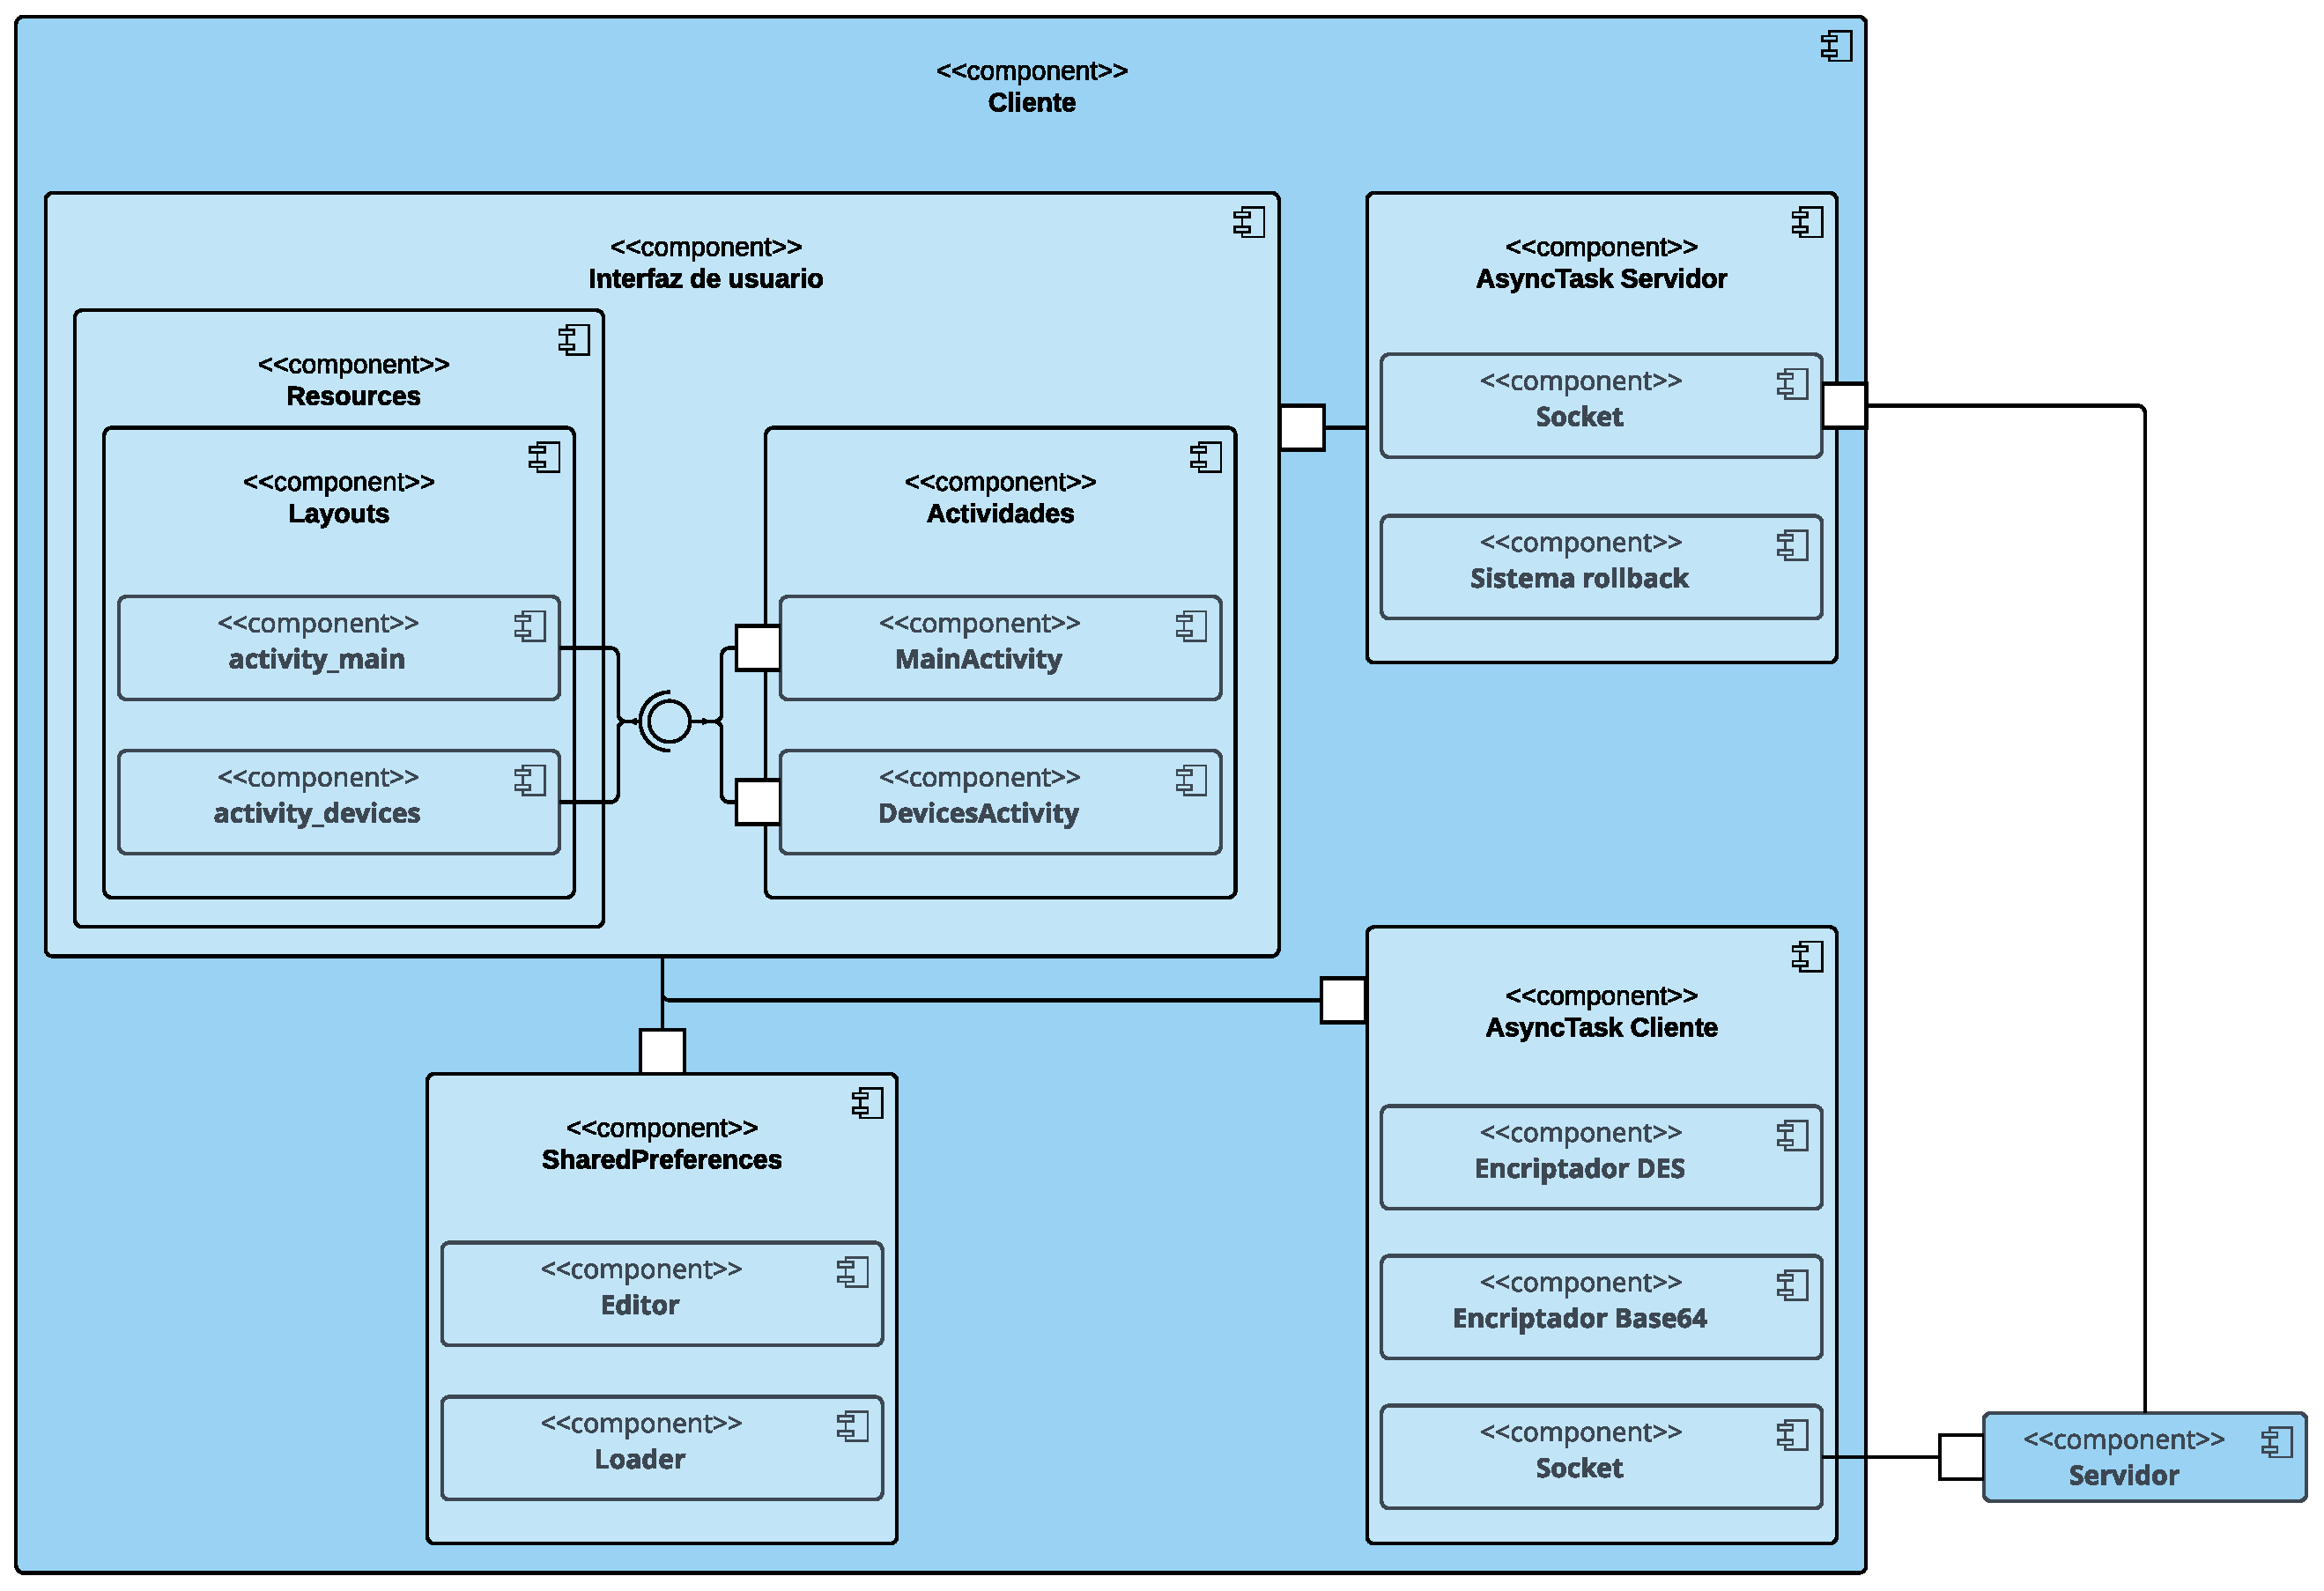
\includegraphics[scale=0.35]{client_diagram.eps}
                \caption{Diagrama de componentes del cliente}
                \label{fig:client_diagram}
            \end{figure}

            La arquitectura del cliente está dividida en tres componentes siguiendo el patrón de arquitectura MVC. Los \textit{Layouts} son renderizados desde el componente \textit{Actividades}, este es el encargado de gestionar la interacción con el usuario, haciendo uso de los componentes \textit{AsyncTask} siempre que sea necesario. El componente \textit{SharedPreferences} es utilizado para el almacenamiento de la configuración del cliente.

            A continuación se explica la función de cada uno de los subcomponentes del sistema:

            \begin{enumerate}
                \item Interfaz de usuario
                    \begin{itemize}
                        \item \textbf{\underline{Actividades}} \\
                            Realiza función de controlador, es el componente encargado de renderizar las vistas haciendo uso de los \textit{Resources} necesarios. Gestiona las entradas del usuario, y a partir de estas se comunica con el sistema servidor a través de los \textit{AsyncTask}.
                        \item \textbf{\underline{Resources}} \\ 
                            Es el componente que representa el conjunto de recursos necesarios para renderizar las vistas de forma correcta, y que estas a su vez, puedan ser gestionadas por las \textit{Actividades}.
                    \end{itemize}
                \item SharedPreferences
                    \begin{itemize}
                        \item \textbf{\underline{Editor}} \\ 
                            Permite almacenar elementos de forma sencilla como elementos clave-valor sin necesidad de utilizar una base de datos.
                        \item \textbf{\underline{Loader}} \\
                            Permiten recuperar los elementos clave-valor almacenados con el \textit{Editor}
                    \end{itemize}
                \item AsynckTask Servidor
                    \begin{itemize}
                        \item \textbf{\underline{Socket}} \\ 
                            Componente mediante el cual se recibe información desde el servidor y provoca cambios parciales en las vistas a detravés del \textit{Sistema rollback}.
                        \item \textbf{\underline{Sistema rollback}} \\
                            Realiza cambios parciales en las vistas a través de las \textit{Actividades}, bloqueando los elementos modificados y devolviéndolos a su estado original en caso de fallo.
                    \end{itemize}
                \item AsynckTask Cliente
                    \begin{itemize}
                        \item \textbf{\underline{Codificador DES}} \\
                            Utilizando la contraseña especificada por el usuario, aplica cifrado \textit{DES} a la información de control que luego es enviada al sistema servidor.
                        \item \textbf{\underline{Codificador Base64}} \\
                            Este componente es el encargado de cifrar en \textit{Base64} los datos obtenidos del \textit{Codificador DES} para que puedan ser enviados al sistema servidor a través del \textit{Socket}.
                        \item \textbf{\underline{Socket}} \\ 
                            Componente mediante el cual se envían los mensajes de control al sistema servidor en función de la entrada del usuario.
                    \end{itemize}
                    Componente que envía mensajes de control al sistema servidor, provoca cambios parciales en las vistas a través de la \textit{Actividad} desde la que es invocado
            \end{enumerate}

            \paragraph{ Estructura del paquete}
            Dado que el protocolo utilizado para la comunicación ente los sistemas cliente y servidor es UDP, los paquetes utilizados portan la cabecera \textit{IP} y adicionalmente los cuatro campos pertenecientes a la cabecera UDP. El campo opcional \textit{Puerto de origen} es completado por la aplicación cliente, permitiendo recibir de vuelta un paquete de confirmación en el mismo socket desde el que ha sido enviado. En la figura \ref{fig:ip_packet} puede observarse la estructura del paquete, se marca en rojo la cabecera \textit{IP}, debajo se encuentra la cabecera UDP, y por último la forma en la que viajan los mensajes de control.

            \begin{figure}[h!]
            \centering
                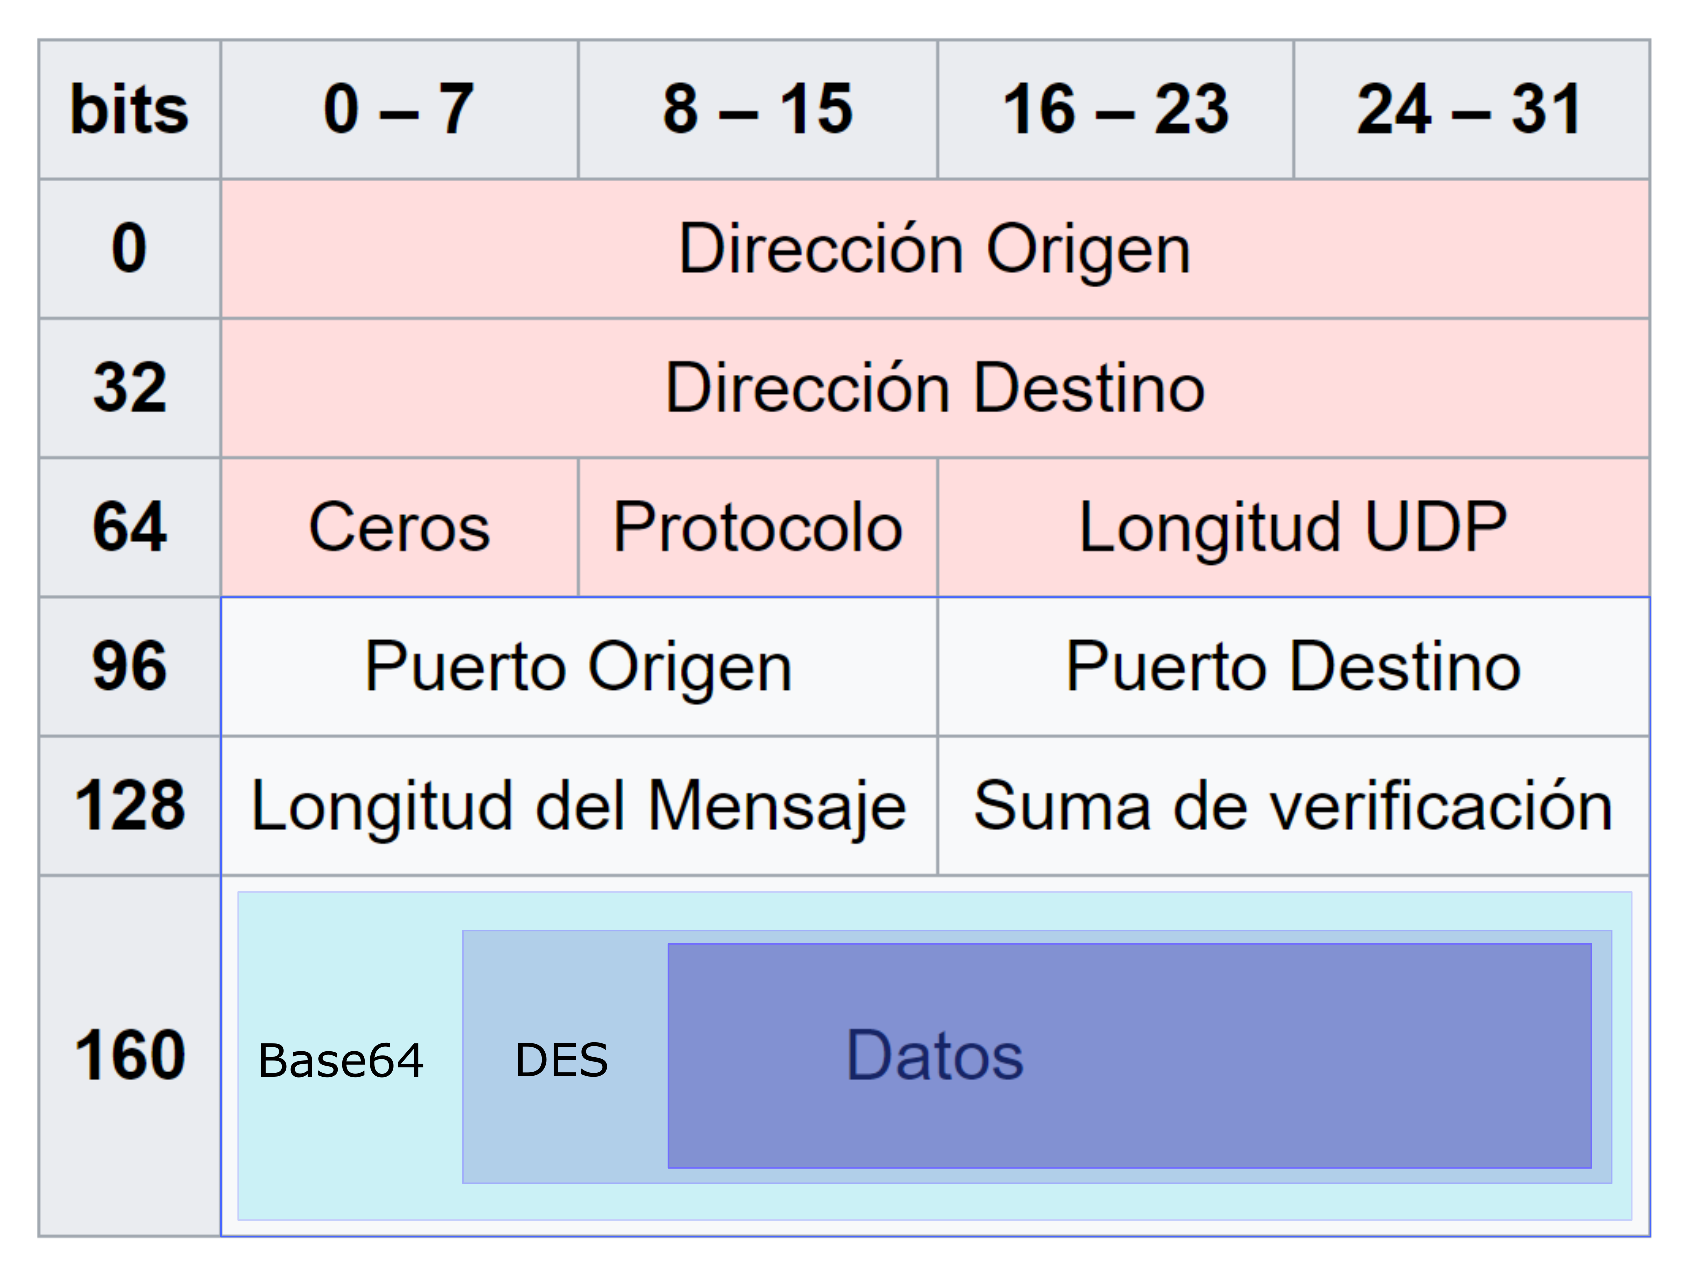
\includegraphics[scale=0.4]{ip_packet.eps}
                \caption{Estructura del paquete}
                \label{fig:ip_packet}
            \end{figure}

            El contenido que viaja cifrado dentro de cada paquete varía en función de la acción que se elige realizar desde el sistema cliente, esta contiene un mensaje de control, y adicionalmente puede contener información necesaria para la acción a realizar. En la tabla \ref{tab:packet_content} se muestra el contenido de los mensajes de control enviados por el cliente.

            \begin{table}[h!]
                \centering
                    \resizebox{\textwidth}{!}{
                        \begin{tabular}{|l|c|c|}
                            \hline
                            \textbf{Acción}                                     &   \textbf{Contenido}      \\         
                            \hline
                            Reiniciar red Wi-Fi                                 &   0                       \\
                            Apagar red Wi-Fi                                    &   1                       \\
                            Encender red Wi-Fi                                  &   2                       \\
                            Deshabilitar filtro MAC                             &   3                       \\
                            Establecer filtro MAC en ``denegar''                &   4                       \\
                            Establecer filtro MAC en ``permitir''               &   5$<$dirección mac$>$    \\
                            Añadir dispositivo al filtro MAC                    &   6$<$dirección mac$>$    \\
                            Eliminar dispositivo del filtro MAC                 &   7                       \\
                            Actualizar configuración                            &   8                       \\
                            Actualizar lista de dispositivos                    &   9                       \\
                            \hline
                        \end{tabular}
                    }
                \caption{Contenido del paquete}
                \label{tab:packet_content}
            \end{table}

            La estructura del mensaje de confirmación es similar, pero en este se omite el cifrado y solamente se envía el mensaje de control, de esta forma se confirma que la acción se ha realizado correctamente. En los casos de ``Actualización'' el componente \textit{AsyncTask Servidor} se mantiene escuchando en el \textit{Socket} determinado hasta que se reciba el mensaje ``done'', que indica que ya han sido enviados todos los paquetes necesarios.

    \subsection{Tecnologías e integración de productos de terceros}
    % describiranse adecuadamente as tecnoloxías utilizadas para o desenvolvemento do traballo, así coma os diversos productos que non son da autoría do/da estudante, xustificando a súa utilización.
        \subsubsection{OpenWRT}
            OpenWRT es una distribución Linux para dispositivos embebidos. En lugar de existir como un firmware estático, OpenWRT proporciona un sistema de archivos totalente modificable con gestión de paquetes, el cual permite sustituir el sistema del proveedor y una mayor personalización del dispositvo. Es el framework perfecto para el desarrollo de una aplicación sin tener que construir todo el firmware que la rodee. Además, este sistema operativo se ha convertido prácticamente en un estándar, soportado por múchos de los dispositivos actuales del mercado, por lo que se utiliza como base para desarrollar esta aplicación.

        \subsubsection{Lenguaje C}
            Es un lenguaje de programación imperativo de prósito general, que destaca por la eficiencia de su código y su popularidad para crear software de sistemas debido a su flexibiliadad y control a muy bajo nivel. Es la opción ideal cuando se desea ahorrar la mayor cantidad de espacio posible en la construcción del software, necesidad común de dispositivos embebidos, y la razón por la que es utilizado en este proyecto.

            \begin{itemize}
                \item \textbf{OpenWRT SDK} \\
                El SDK es un conjunto de herramientas de programación reubicables y precompiladas que permiten la compilación cruzada de paquetes para el espacio de usuario de OpenWRT sin tener que compilar todo el sistema desde cero.

                \item \textbf{uClibc} \\
                    Es una librería C para el desarrollo de sistemas Linux embebidos, es más pequeña que la librería \textit{glibc} (GNU C Library) y soporta prácticamente todas las aplicaciones que son desarrolladas con esta. \textit{uClibc} es capaz de gestionar librerías compartidas e hilos, además de funcionar con procesadores de varias arquitectura, entre las que se incluyen amd64, ARM, mips/mipsel, alpha, PowerPC y SH.

                \item \textbf{OpenSSL} \\
                    Es un proyecto de código abierto que implementa la una librería criptográfica de propósito general. Provee un conjuto de herramientas robusto, de nivel comercial, para los protocolos SSL/TLS.
            \end{itemize}
            
        \subsubsection{OpenVPN}
            Es un proyecto basado en software libre, que proporciona una solución de conectividad punto a punto, con validación gerárquica de usuarios y dispositivos conectados remotamente. Hace uso del protocolo SSL para crear redes privadas virtuales (VPN) que permiten mantener la privacidad generando un túnel entre dos dispositivos separados geográficamente.

        \subsubsection{Sed}
            Es una utilidad unix, un editor de flujo capaz de analizar y transformar textos utilizando un simple y compacto lenguaje de programación. Permite el uso de expresiones regulares y tratamiento de archivos con un gran número de líneas de forma rápida. En este sistema \textit{sed} es utilizado para llevar a cabo los cambios en los archivos de configuración proporcionados por OpenWRT.

        \subsubsection{Latex} \label{sec:latex}
            Es un sistema de tipografía de alta calidad, incluye mecanismos diseñados para la creación de documentación científica y técnica por lo que se ha convertido en el estándar de facto a la hora de desarrollar esta tarea. Está concebido como software libre, y cuenta con múltiples librerías que añaden funcionalidades comunmente necesarias para la creación de estos doumentos. La documentación del desarrollo de este sistema está desarrollado con esta tecnología debido al conjunto de ventajas de estilo y edición que ofrece frente a otras tecnologías libres.

        \subsubsection{Java}
            Es un lenguaje de programación orientado a objetos, compilado, de propósito general y alto nivel. Es utilizado para soluciones web, cliente-servidor, sistemas distribuidos, etc. además de ser el principal lenguaje para el desarrollo de aplicaciones móviles Android, razón por la que es utilizado en el desarrollo de este sistema.

        \subsubsection{Git} \label{sec:git}
            Es un sistema de control versiones distribuido diseñado para controlar proyectos de cualquier tamaño con rapidez y eficacia. Es de código abierto y ofrece medios para guardar, analizar y revertir cambios realizados en versiones actuales y anteriores, además del control de ramas que permite mantener y trabajar en más de una versión de un proyecto de forma simultánea. Su uso en el desarrollo de este sistema viene justificado por las diferentes iteraciones/sprints que se llevan a cabo y el control de versiones necesario para su gestión.

    \subsection{Herramientas} 
        \subsubsection{Atom}
            Es un editor de texto de código abierto desarrollado por GitHub Inc., escrito en JavaScript, moderno, accesible y modificable en su totalidad. Es completamente personalizable, de forma que brinda el entorno de trabajo más cómodo y productivo posible, sin necesidad de modificar ningún archivo de configuración durante el desarrollo de proyectos. Cuenta con una muy amplia gama de paquetes, también de código abierto, que añaden y mejoran funcionalidades del editor.

        \subsubsection{Visual Studio Code}
            Es una herramienta desarrollada por Microsoft que combina las simplicidad de un editor de texto con lo que necesitan los desarrolladores para su ciclo básico \textit{``edit-build-debug''}. Visual Studio Code provee soporte exhaustivo para la creación y depuración de código, además de un modelo extendible y una integración de bajo consumo de recursos con las herramientas existentes.

        \subsubsection{TeX Live}
            Es un una distribución libre para los sistemas de tipografía TeX (\ref{sec:latex}). Está disponible para Linux y Windows incluyendo la mayoría de programas, micro paquetes y fuentes que son software libre. Actualmente es la distribución por defecto de esta tecnología en múltiples distribuciones Linux como openSUSE, Fedora, Debian, Ubuntu y Gentoo, además de ofrecer soporte para múltiples idiomas.

        \subsubsection{Android Studio}
            Es el IDE (Integrated development environment) oficial para la creación aplicaciones Android. Ofrece herramientas para la edición de códigos de primer nivel, depuración, control de rendimiento y compilación instantánea. Provee de un emulador Android que permite comprobar el funcionamiento del código de forma rápida, y brinda un conjunto de opciones dinámicamente configurables en cuanto a tamaño, prestaciones y control de sensores. Posee integración condiferentes sitemas actuales y cuenta con soporte para librerías externas configurables para su compilación junto con la aplicación.

        \subsubsection{GitHub}
            Es una plataforma colaborativa de control de vesiones online basada en Git(\ref{sec:git}) y desarrollada por GitHub Inc. Ofrece todas las funcionalidades de gestión de códigos que ofrece Git, así como sus propias características basadas en la web. Provee control de acceso y varias opciones colaborativas como el control de errores, petición de funcionalidades, gestión de tareas y wikis. La plataforma cuenta con un servicio de pago que permite la creación de repositorios privados, este servicio está disponible de forma gratuita junto a un conjunto de herramientas de desarrollo que la empresa ofrece en un paquete para estudiantes verificados.

        \subsubsection{Lucidchart}
            Es una aplicación online enfocada a la creación de diagramas profesionales desde una interfaz web. Es una herramienta realmente cómoda a la hora de documentar proyectos grandes debido a lo sencillo y amigable de su entorno. Además, brinda integración con diferentes aplicaciones externas como Dropbox, Slack y Microsoft Office. 

        \subsubsection{Inkscape}
            Es un editor profesional de gráficos vectoriales disponible para Windows, Mac OS X y Linux. Es de código abierto y soporta una gran variedad de formatos, entre los que se incluye \textit{.eps}, el formato utilizado por latex. Además brinda una amplia variedad de herramientas para realizar trazado vectorial, manipulación de objetos y edición de textos.

        \subsubsection{OpenVPN for Andorid}
            Es una aplicación gratuita disponible en la tienda online de \textit{Google}. Permite utilizar OpenVPN en dispositivos móviles para crear conexiones punto a punto de forma segura. Todo el tráfico generado entre estos puntos es transportado en paquetes cifrados, haciendo uso de certificados SSL.


\cleardoublepage \section{Especificación y análisis de requisitos} \label{sec:req}
% describiranse os requisitos necesarios, tanto funcionais como non funcionais. Incluiranse os aspectos máis relevantes correspondentes á análise do traballo realizado.
    
    \subsection{Casos de uso}
        En la figura \ref{fig:case_use_diagram} se muestra el diagrama de casos de uso del que dispone el sistema.
        \begin{figure}[h!]
        \centering
            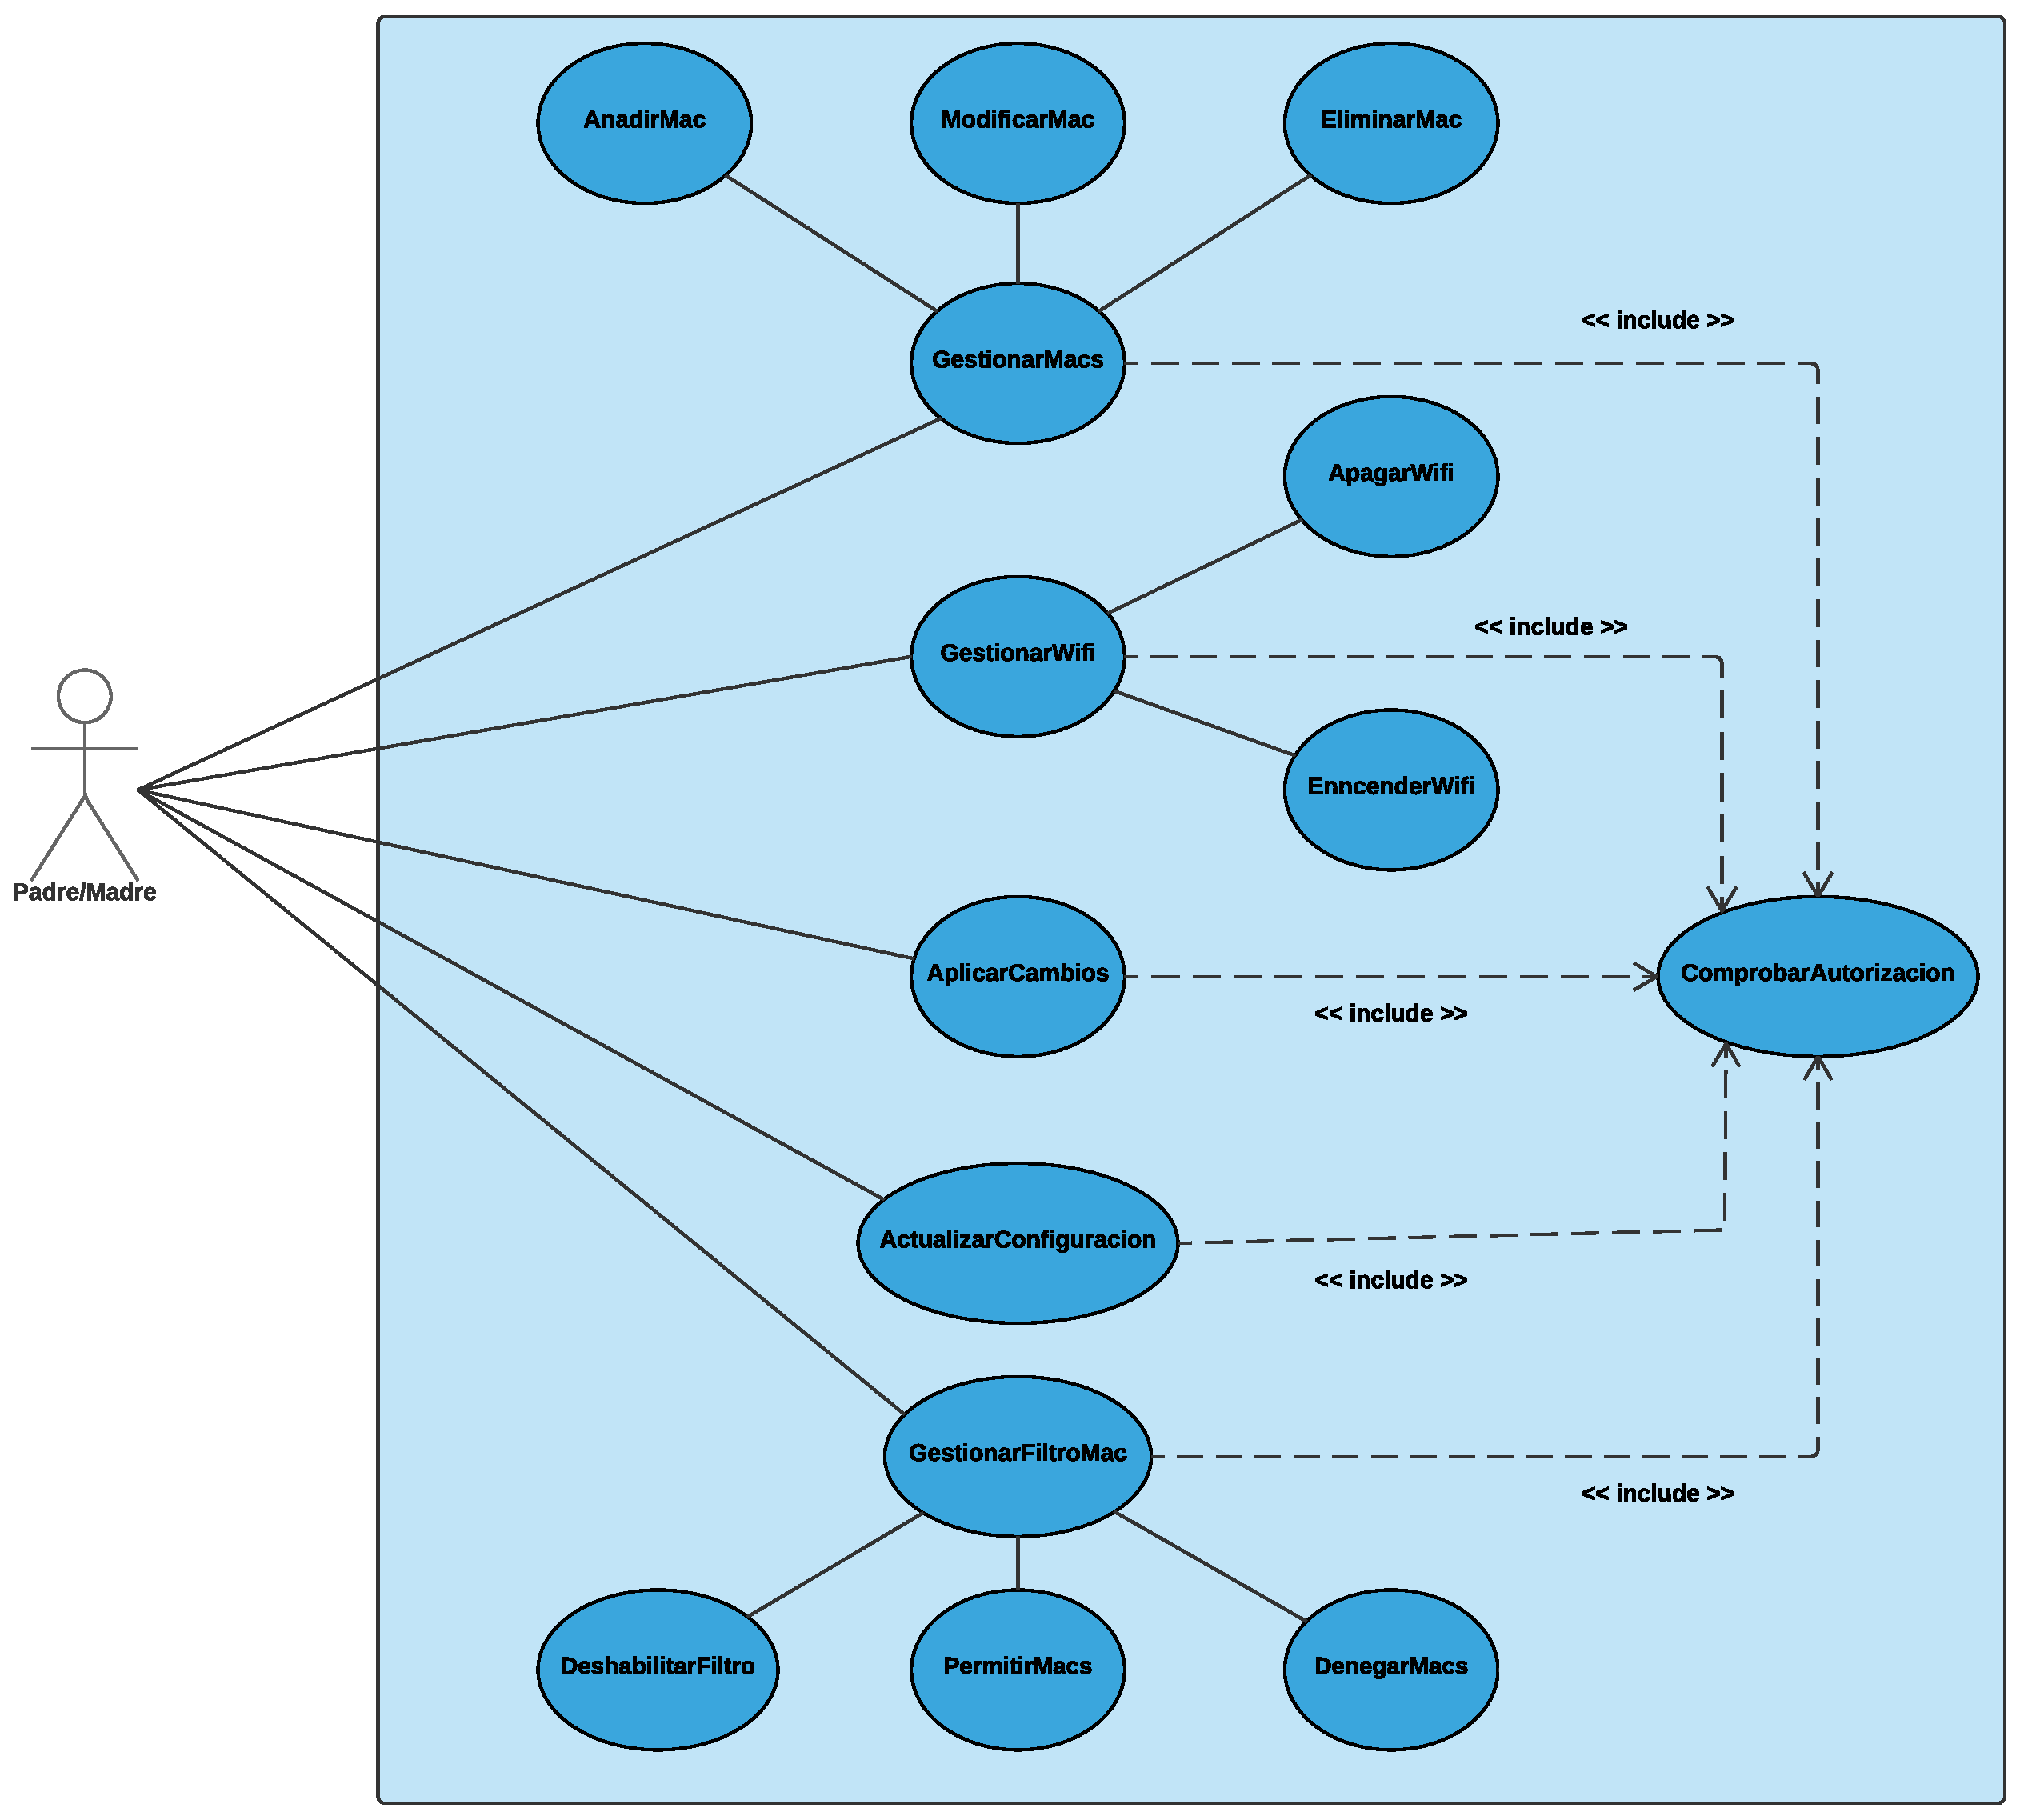
\includegraphics[scale=0.35]{case_use_diagram.eps}
            \caption{Diagrama de casos de uso}
            \label{fig:case_use_diagram}
        \end{figure}
    
    \subsection{Requisitos funcionales}
        \begin{itemize}
            \item \textbf{\underline{Apagado y encendido de la red Wi-Fi}} \\
            Enciende y apaga el red Wi-Fi del router servidor. 
            \item \textbf{\underline{Configuración del filtro MAC}} \\
            Gestiona el estado del filtro de direcciones MAC.
            \item \textbf{\underline{Gestión de dispositivos}} \\
            Permite añadir, eliminar y modificar dispositivos al sistema.
            \item \textbf{\underline{Soporte de idiomas}} \\
            Cambiar el idioma de la interfaz.
        \end{itemize}
    
    \subsection{Requisitos no funcionales}
        \begin{itemize}
            \item \textbf{\underline{Seguridad:}}
            El sistema cuenta con mecanismos de cifrado DES y el uso de túneles VPN capaces de restringir el acceso de los dispositivos no autorizados y evitar las replicación de paquetes..
            \item \textbf{\underline{Disponibilidad:}}
            El sistema se mantiene a la espera de peticiones de los clientes en todo momento, tanto desde la Interfaz Wi-Fi como de la interfaz WAN.
            \item \textbf{\underline{Accesibilidad:}}
            El sistema cuenta con una interfaz gráfica sencilla e intuitiva que permite su uso a los usuarios más inexpertos
            \item \textbf{\underline{Portabilidad:}}
            El sistema puede ser utilizado en dispositivos móviles Android, con los que se pueden acceder desde cualquier parte del mundo siempre que exista conectividad con internet.
            \item \textbf{\underline{Usabilidad:}}
            El sistema mantiene un tiempo de respuesta rápido, teniendo en cuenta la velocidad de la conexión a Internet, brinda toda la información necesaria y mantiene un conjunto de tonalidades discreto.
            \item \textbf{\underline{Rendimiento:}}
            El sistema funciona de forma fluida, mantenienndo un bajo consumo de recursos en los dispositivos.
        \end{itemize}

\cleardoublepage \section{Diseño de software} \label{sec:dis}
% (estático e dinámico) ou do hardware: indicaranse os aspectos máis relevantes correspondentes ao deseño do traballo realizado
% estatico -> diagrama de clases
% dinamico -> diagrama de secuencia
    \subsection{Diseño estático}
        Dado que el sistema servidor está desarrollado utilizando el lenguaje C, no dispone de clases que puedan ser representadas en un diagrama de este tipo. La aproximación más cercana a un diseño estático, que puede ser obtenida de este sistema, es su representación en un diagrama de paquetes, el cual puede ser observado en la figura \ref{fig:server_diagram}, ya expuesta en la sección \ref{sec:arq}.

        El sistema servidor está desarrollado en Android, por lo que sí cuenta con clases para realizar una representación en un diagrama. La figura \ref{fig:class_diagram} muestra el diagrama de clases del sistema cliente.
        

    \subsection{Diseño dinámico}
    En la imagen \ref{fig:main_activity_sequence_diagram} se puede observar el diagrama de secuencia general del sistema, donde se muestra la interacción entre los objetos que lo componen. En esta representación pueden variar el mensaje enviado, la actividad y el servidor de configuración, manteniendo la misma forma en la que interactúan.

    \begin{figure}[h!]
    \centering
        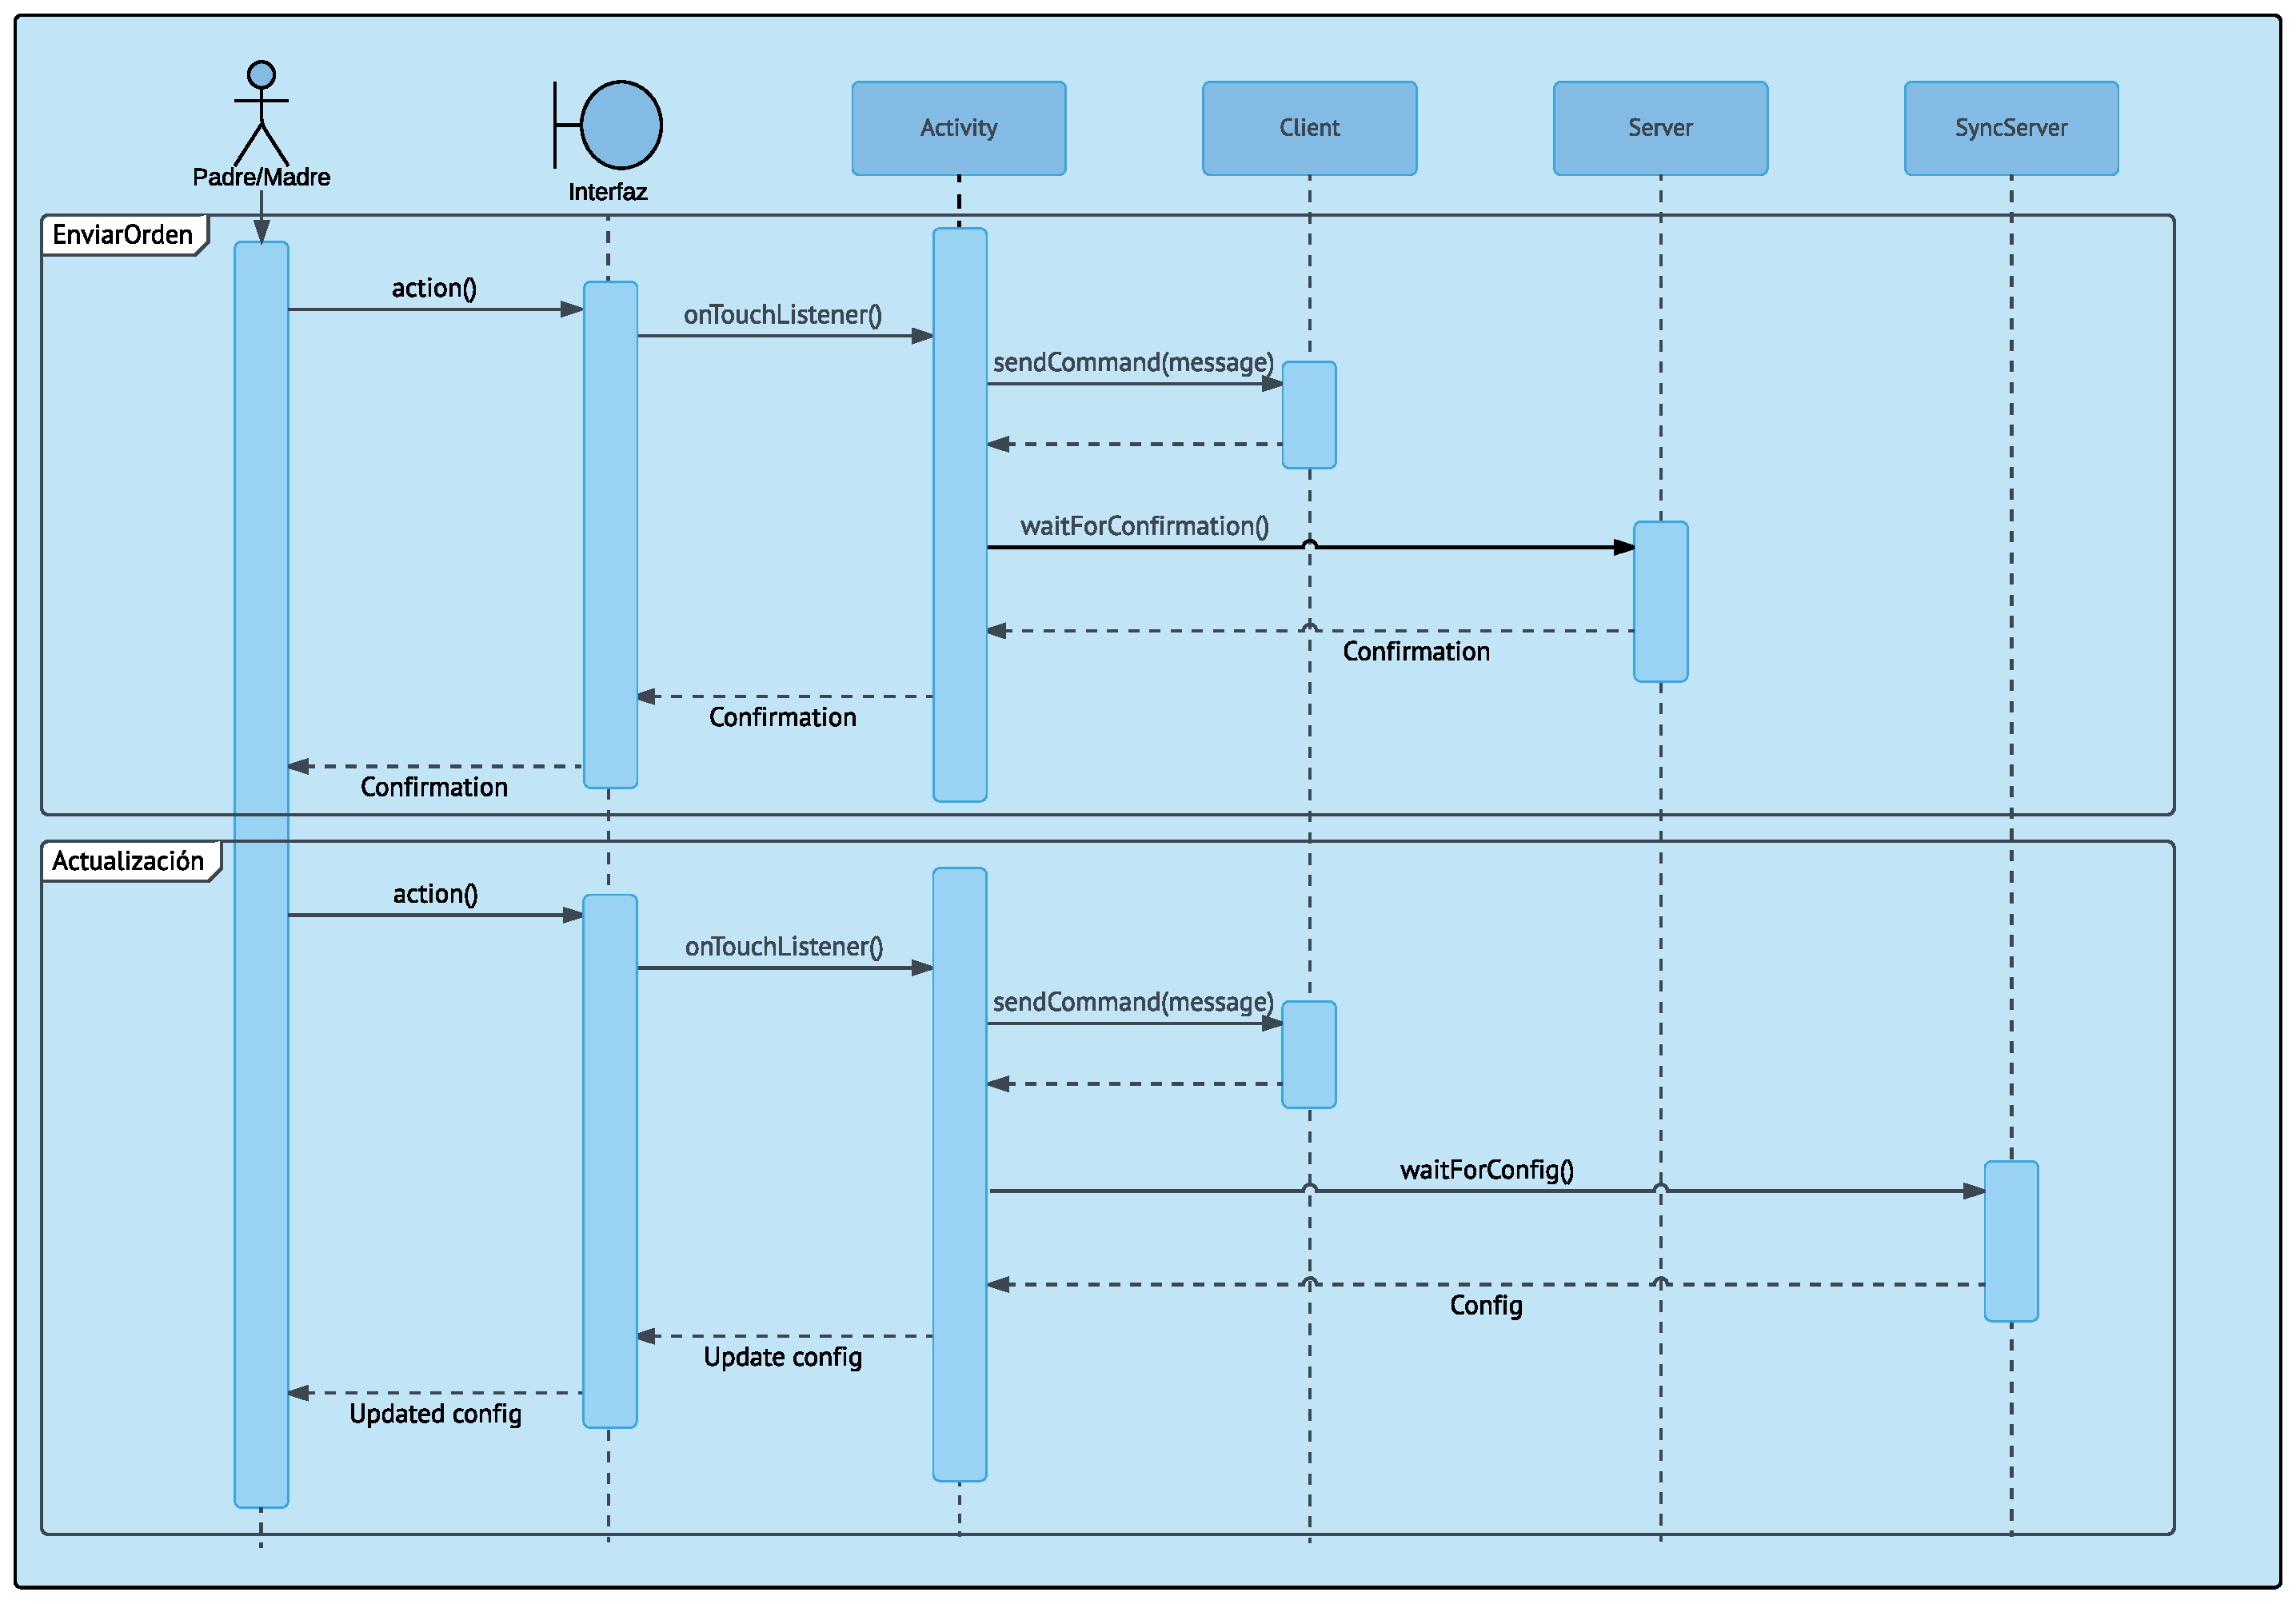
\includegraphics[scale=0.32]{main_activity_sequence_diagram.eps}
        \caption{Diagrama secuencia de actividades}
        \label{fig:main_activity_sequence_diagram}
    \end{figure}

    En la imagen \ref{fig:device_management_sequence_diagram} se muestra un diagrama de secuencia que representa la interacción de las clases para los casos de uso de gestión de dispositivos.
    \begin{figure}[h!]
    \centering
        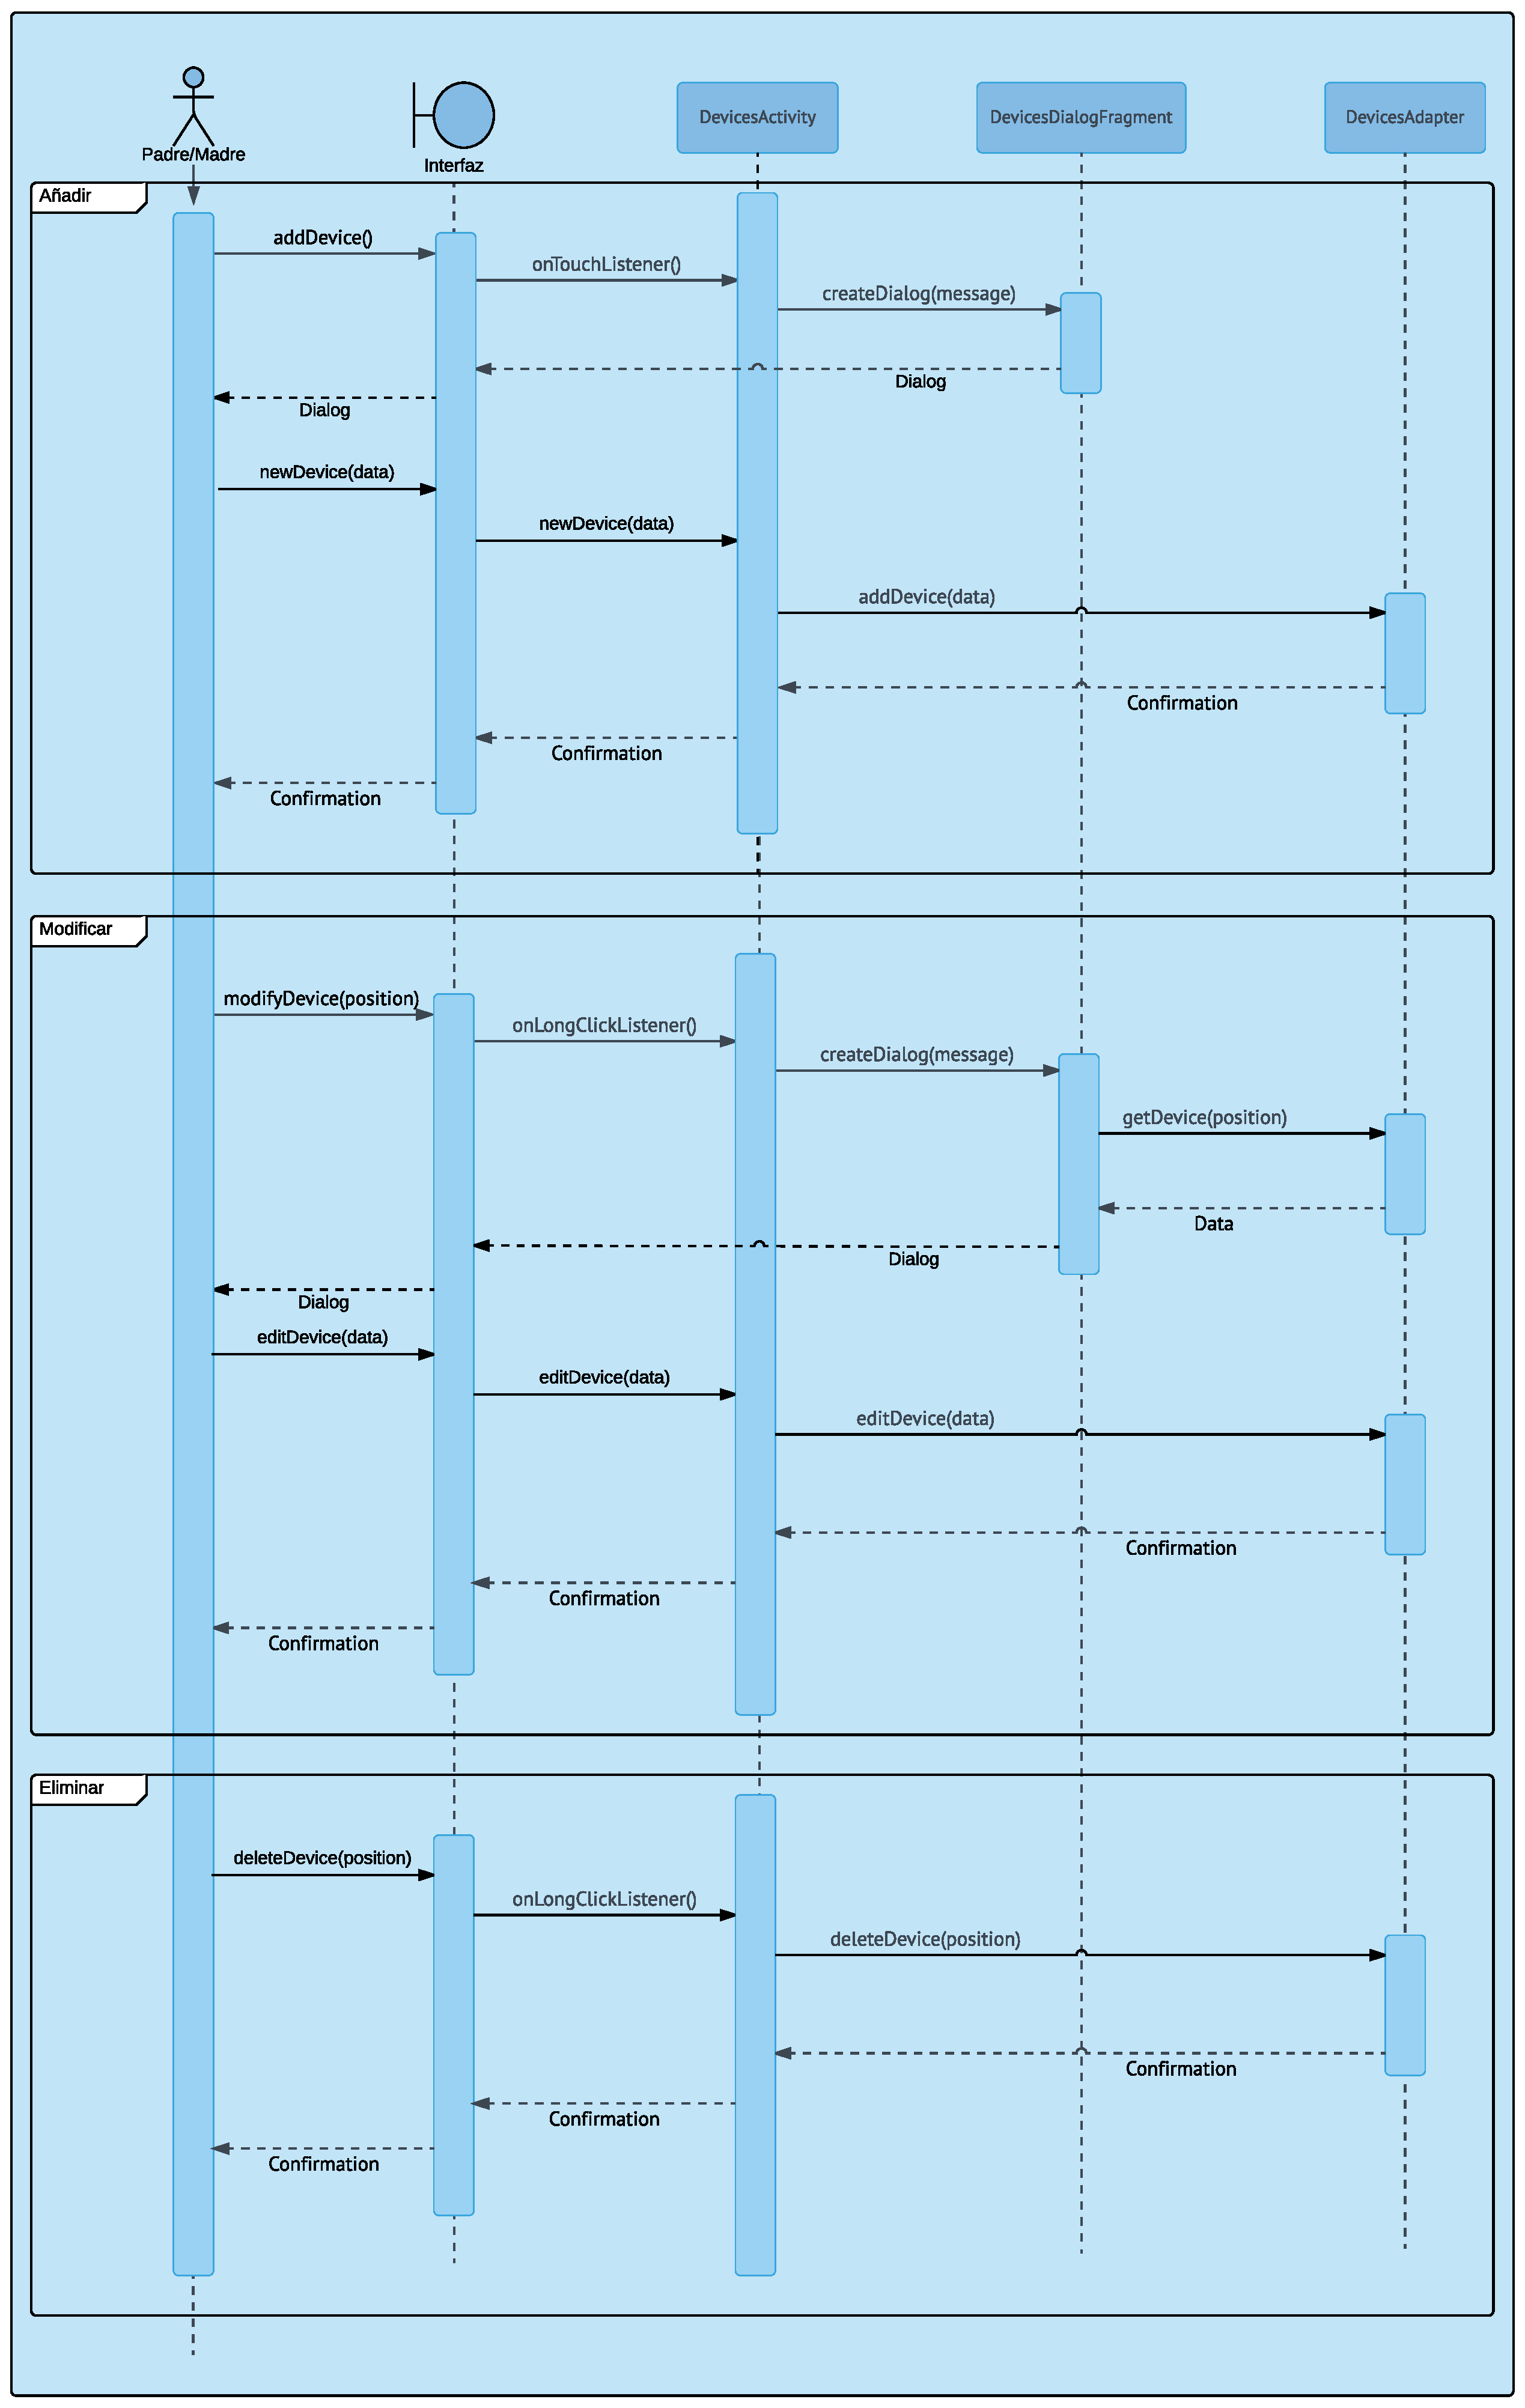
\includegraphics[scale=0.35]{device_management_sequence_diagram.eps}
        \caption{Diagrama de secuencia de gestión de dispositivos}
        \label{fig:device_management_sequence_diagram}
    \end{figure}

\cleardoublepage \section{Gestión de datos e información} \label{sec:dat}
% Xestión de datos e información: describiranse os métodos ou técnicas empregadas para xestionar tanto os datos coma o resto de información relevante.
    Ya que el objetivo es la creación un mecanismo de control para accesos a la red Wi-Fi, el sistema que se plantea no cuenta con bases de datos para almacenar información, sin embargo, se necesita una forma de guardar las configuraciones utilizadas.
    
    \subsection{Servidor}
        En el dispositivo servidor, para hacer uso de los mecanismos que brinda OpenWRT (orientados la gestión de sus funcionalidades), se cuenta con un conjunto de archivos de configuración ubicados en la carpeta \textit{/etc/config}. En especial, se hace uso del fichero \textit{wireless}, donde se almacenan las configuraciones hardware y software que son utilizadas para el funcionamiento la red Wi-Fi. A continuación se muestra un ejemplo de este:

        \begin{lstlisting}[caption=/etc/config/wireless, language=bash]
    config wifi-device 'radio0'
            option type 'mac80211'
            option hwmode '11g'
            option path 'pci0000:00/0000:00:01.0/ssb0:0'
            option disabled '0'
            option channel '4'
            option txpower '20'
            option country '00'

    config wifi-iface
            option network 'wwan'
            option encryption 'psk2'
            option device 'radio0'
            option ssid 'TFG_AccessPoint'
            option mode 'ap'
            option key 'wifitesting'

            option macfilter `deny'
            list maclist 'B1:EE:A1:04:23:4E'
            list maclist 'B4:5D:83:4A:1B:50'
            list maclist '0E:00:C1:FA:4E:98'
        \end{lstlisting}

        El parámetro \textit{wifi-device} indica la configuración de un dispositivo físico conectado al sistema, y al cual se le aplican las opciones que se definen debajo. En estas opciones se especifican parámetros como el tipo de dispositivo, la potencia y el canal que utilizará.

        El parámetro \textit{wifi-iface} indica la configuración de una interfaz inalámbrica, especificando en las opciones el dispositivo físico y la red OpenWRT (ya definidos) a la que estará vinculada. Además, también se definen opciones como el mecanismo de seguridad y el modo de operación del controlador de red. El sistema que se desarrolla, hace uso de las funciones que se encuentran al final del ejemplo.
        
        \begin{itemize}
            \item \textbf{\underline{mactiflter:}} Indica la configuración a adoptar por el filtro MAC, esta se especifica entre comillas simples, y puede ser \textit{deny} o \textit{allow}. Para indicar que el filtro debe está desactivado se elimina toda la línea.
            \item \textbf{\underline{list maclist:}} Es utilizada para especificar las direcciones MAC a las que se les va a aplicar el filtro, se pueden definir tantas opciones \textit{list maclist} como sea necesario.
        \end{itemize}

    \subsection{Cliente}
        En el dispositivo cliente, las configuraciones que se almacenan son las relacionadas a la conexión: \textit{Dirección IP}, \textit{Puerto} y \textit{Contraseña}, así como los \textit{Dispositivos} añadidos a la aplicación para gestionar el filtro MAC. También son almacenados los \textit{Estados} de los elementos de la interfaz de usuario que son utilizados para controlar el sistema.

        Para gestionar estos datos se utiliza \textit{SharedPreferences}, una forma de almacenamiento \textit{Clave-Valor} ofrecida por Android. Un objeto de este tipo tiene asociado un archivo donde se almacenan dichos pares, y proporciona métodos simples para gestionar su lectura y escritura.
        
        Los procesos de lectura y escritura se realizan dentro de \textit{onResume()} y \textit{onPause()} respectivamente. El primero es ejecutado cuando la actividad es creada, iniciada o reanudada, mientras que el segundo es ejecutado cuando la actividad por cualquier motivo quede suspendida, la aplicación sea detenida o el proceso destruido. La figura \ref{fig:android_lifecycle} muestra el orden de ejecución de los métodos en una actividad Android.
        
        \begin{figure}[h!]
            \centering
                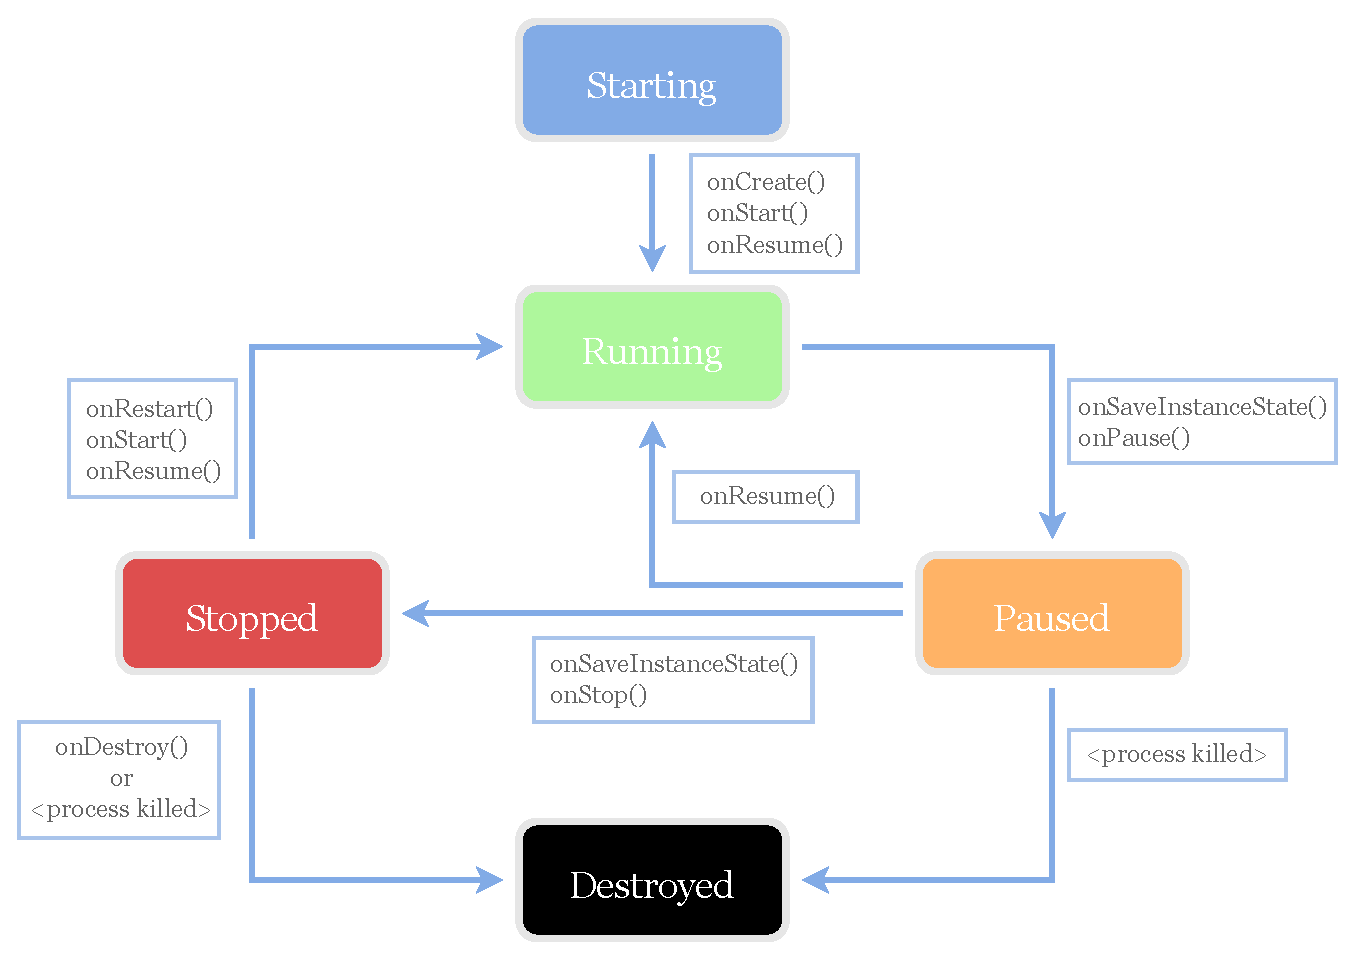
\includegraphics[scale=0.7]{android_lifecycle.eps}
                \caption{Ciclo de vida de actividades Android}
                \label{fig:android_lifecycle}
        \end{figure}

\cleardoublepage \section{Pruebas llevadas a cabo} \label{sec:pru}
% describiranse as probas realizadas aos distintos niveis para
% garantir o correcto funcionamento do software ou do hardware.
    \subsection{Explicación de las pruebas}
    Muchos de los paradigmas de programación ágil abarcan el concepto de prueba unitaria. Pruebas programadas en el mismo lenguaje que se escribe la aplicación y que permiten comprobar el funcionamiento de una unidad de código. La metodología \textit{SCRUM} normalmente es utilizada con pruebas automatizadas que son creadas específicamente para cada sprint, y ejecutadas al final de éste, junto con las que anteriormente hayan finalizado de forma satisfactoria. Los nuevos componentes desarrollados sólo son considerados correctos cuando todas las pruebas están validadas, permitiendo que el código resultante esté libre de errores y no comprometa el funcionamiento del resto del sistema creado hasta el momento.

    \subsection{Pruebas de conectividad}
    Debido a que en este proyecto se lleva a cabo el desarrollo de dos aplicaciones diferentes que deben intercambiar paquetes UDP entre sí, es necesario un conjunto de pruebas que permita verificar la conectividad entre ambas. Por tanto, se ha decidido utilizar pruebas unitarias desarrolladas en Android Studio que comprueben, mediante el propio sistema de confirmación de la aplicación cliente, su funcionamiento, y permitan así verificar si el paquete es enviado, recibido y confirmado.

    \subsection{Pruebas de entrada}
    Las pruebas en las aplicaciones independientes se realizan de forma manual, introduciendo valores correctos e incorrectos en los campos a comprobar. En el servidor se introducen estos valores como parámetros durante su proceso de inicio, y en el cliente se comprueban los campos de texto, tanto los encargados de la configuración de la conexión, como los de gestión de dispositivos.

    \subsection{Pruebas de encriptación}
    El funcinamiento del sistema de encriptación entre cliente y servidor es verificado mediente la prueba unitaria de conectividad, especificando valores correctos e incorrectos para el campo contraseña tanto de la aplicación como del servidor. Para realizar pruebas en los sistemas por separado se hace uso de la librería \textit{OpenSSL}, los valores obtenidos como resultado de la aplicación deben ser iguales a los generados con esta librería desde la consola de comandos, siempre y cuando los parámetros utilizados sean los mismos. 

\cleardoublepage \section{Manual de usuario} \label{sec:man}
    \subsection{Requisitos mínimos}
        Para poder utilizar el sistema \textbf{Wifither} se debe cumplir un conjunto de requisitos, los cuales están especificados a continuación.

        \begin{itemize}
            \item Equipo con una distrubución GNU/Linux para compilar paquete. Ubuntu como subsistema de Windows, BSD o MacOS no están oficialmente soportados, aunque suelen dar buenos resultados. Cygwin no está soportado debido al sistema de archivos que utiliza, que no es capaz de distinguir entre mayúsculas y minúsculas.
            \item Router con sistema operativo OpenWRT donde se ejecutará el servicio servidor.
            \item Dispositivo móvil con sistema operativo Android donde se instalará la aplicación cliente.
            \item Conexión a Internet tanto en el router como en el dispositivo móvil.
        \end{itemize}

        Aunque muchas de las dependencias necesarias suelen venir por defecto instaladas en diferentes sistemas operativos, es necesario que todas estén instaladas y funcionales. En el anexo \todo{referenciar} se muestra una tabla con las dependencias y el nombre de los paquetes en distribuciones \textit{Debian-like} y \textit{Arch-Linux}.

        Para instalar paquetes en distribuciones \textit{Debian-like} su utiliza el siguiente comando.
        Es necesario que el usuario desde el que se ejecute el comando de instalación cuente con los permisos necesarios para llevar a cabo dicha acción.

        \begin{lstlisting}[language=bash]
    $ apt-get install <paquete>
        \end{lstlisting}

        Varios paquetes pueden ser instalados a la vez utilizando el comando solo una vez.
        Ejemplo:

        \begin{lstlisting}[language=bash]
    $ apt-get install libncurses5-dev subversion gawk
        \end{lstlisting}

    \subsection{Manual de instalación}
        \subsubsection{Compilar el paquete Wifither para OpenWRT}
            Para preparar la compilación cruzada, se debedescargar desde la página web oficial de OpenWRT (\url{https://downloads.openwrt.org}) el SDK correspondiente al modelo del dispositivo y la versión del sistema en el que se desea instalar el paquete. Una vez descargado, se debe descomprimir el archivo y copiar el código fuente dentro de la carpeta \textit{build} del SDK. Luego, desde la carpeta raíz del SDK, se procede ejecutar los siguientes comandos para preparar las librerías que utiliza \textbf{Wifither}.

            \begin{lstlisting}[language=bash]
    $ ./scripts/feeds update
    $ ./scripts/feeds install uclibcxx
    $ ./scripts/feeds install libopenssl
            \end{lstlisting}

            Una vez esté todo preparado, se debe ejecutar el comando \textit{make} para llevar a cabo la compilación. El paquete resultante se almacena en \textit{SDK/bin/$<$modelo-router$>$/packages/base} con el nombre \textit{wifither 1 $<$modelo-router$>$.ipk}.


        \subsubsection{Instalación del servicio servidor en e router}
            En este apartado se explica cómo instalar el paquete \textit{.ipk} resultante de la compilación, en el router con OpwenWRT, y cómo iniciar el servicio y configurarlo para que se inicie automáticamente cada vez que arranque el router.

            En primer lugar se debe copiar el paquete al router donde se instalará, para ello se puede utilizar cualquier protocolo de red que permita la transferencia de archivos, en esta guía se explica cómo copiarlo mediante el uso de \textit{scp}. Para realizar este proceso, se debe especificar la ruta donde se encuetra el paquete, el usuario y el equipo remoto al que se desea copiar, además de la ruta donde se desea almacenar en ese equipo.

            \begin{lstlisting}[language=bash]
    $ scp <ruta-paquete> <usuario>@<equipo-remoto>:<ruta-almacenamiento>
            \end{lstlisting}

            Un ejemplo de la ejecución del comando:
            \begin{lstlisting}[language=bash]
    $ scp bin/brcm63xx/packages/base/wifither_1_brcm63xx.ipk root@192.168.0.4:/root/wifither
            \end{lstlisting}

            Una vez el paquete está en el router, este podrá ser instalado utilizando el gestor de paquetes de OpenWRT \textit{opkg}
            \begin{lstlisting}[language=bash]
    $ opkg install <ruta-paquete>
            \end{lstlisting}

            Para iniciar el servicio después de haberlo instalado se ejecutará \textit{wifiter} especificando el puerto en el que se desea recibir los paquetes y una contraseña que contenga al menos ocho caracteres.

            Ejemplo:
            \begin{lstlisting}[language=bash]
    $ wifither 4848 Potato12
            \end{lstlisting}

            Para configurar el equipo, de forma que Wifither siempre se inicie al arrancar el sistema, se debe editar el archivo \textit{/etc/rc.local} añadiendo la ejecución del servicio antes de la línea \textit{exit 0}

            \begin{lstlisting}[language=bash]
    # Put your custom commands here that should be executed once
    # the system init finished. By default this file does nothing.

    wifither 4848 Potato12

    exit 0
            \end{lstlisting}


        \subsubsection{Instalación de la aplicación móvil}
            Para realizar la instalación de la aplicación en el móvil existen dos opciones, utilizar la aplicación ya compilada \textit{.apk} o compilarla e instalarla directamente desde \textit{Android Studio}
            
            \begin{enumerate}
                \item \textbf{\underline{Instalación del .apk}} \\
                Es necesario que el archivo \textit{.apk} debe estar almacenado en el dispositivo móvil, para esto se puede conectar el dispositivo directamente al ordenador utilizando un cable USB.

                Para llevar a cabo la instalación debe estar activada la opción \textit{Fuentes desconocidas}, que se encuentra en el apartado \textit{Seguridad} de los ajustes del sistema Android. Esto hace que sea posible la instalación de aplicaciones que provengan de fuentes no oficiales.

                Una vez realizados los pasos anteriores, ir hasta la ubicación del archivo \textit{.apk}, pulsar sobre él y aceptar la instalación.

                \item \textbf{\underline{Compilar e instalar desde Android Studio}} \\
                Para poder instalar aplicaciones utilizando este método es necesario que el dispositivo móvil esté conectado al ordenador mediante un cable USB y que esté activada la opción \textit{Depuración USB}, que se encuentra en el apartado \textit{Opciones de desarrollador} de los ajustes del sistema Android.

                \textbf{NOTA:} Las opciones de desarrollador están deshabilitadas por defecto en la mayoría de dispositivos Android, para habilitarla es necesario pulsar diez (10) veces sobre el \textit{Número de compilación}, que se encuentra en el apartado \textit{Acerca del dispositivo} de los ajuste del sistema Android.

                En la barra de menús de Android Studio, ir a \textit{File} y luego a la opción \textit{Open}, allí buscar y abrir la carpeta con el código fuente de la aplicación. Una vez haya cargado el proyecto, ir la opción \textit{Run `app'} que se encuentra en el menú \textit{Run} y se selecciona el dispositivo.
                
                \textbf{NOTA:} Es importante aceptar en el dispositivo la clave RSA, esto permite que Android Studio pueda conectarse al dispositivo.

                Tras realizar los pasos anteriores, el código fuente debe haber quedado compilado, instalado y ejecutado en el dispositivo conectado.
            \end{enumerate}

        \subsubsection{DNS Dinámico}
            El DNS dinámico o DDNS, como suele ser llamado es un servicio que permite la actualización en tiempo real de la información sobre nombres de dominio situada en un servidor de nombres, en otras palabras, permite asociar a un nombre de dominio una dirección IP estática, para esto es necesario utilizar un proveedor de direcciones dinámicas, es este caso se hará uso de \url{no-ip.org}.

            El paso incial es la creación de un a cuenta de usuario en la web, esto se realiza rellenando el formulario de registro con los datos necesarios. Posteriormente se debe acceder al apartado \textit{Dinamic-DNS}, donde se selecconará un nombre de domino y se especificará la dirección IP pública asignada a la interfaz WAN del router servidor.

            En el router será necesaria la instalación de un paquete de gestión de DDNS, para realizarlo se ejecutan los siguientes comandos desde la consola del:

            \begin{lstlisting}[language=bash]
    opkg update
    opkg install ddns-scripts
    opkg install ddns-scripts_xxxxx
            \end{lstlisting}

            Una vez haya sido instalado el paquete se deberá proceder a su configuración, ésta será la que permita que el router informe al servidor de nombres en caso de un cambio de IP por parte del proveedor de Internet. Para realizar la configuración se ejecutan los siguientes comandos, indicando la información necesaria en cada caso
            
            \begin{lstlisting}[language=bash]
    uci set ddns.myddns.service_name='<proveedor ddns>'
    uci set ddns.myddns.domain='<nombre de dominio seleccionado>'
    uci set ddns.myddns.username='<nombre de usuario>'
    uci set ddns.myddns.password='<contrasena>'
    uci set ddns.myddns.interface='wan'
    uci set ddns.myddns.enabled='1'
    uci commit ddns	
            \end{lstlisting}

        \subsubsection{Configuración de una VPN}
            En este apartado se explica la creación y configuración de una VPN en modo túnel entre el router y el dispositivo móvil, mediante la utilización de OpenVPN. Este paso es totalmente opcional, ya que el sistema no lo necesita para su correcto funcionamiento, sin embargo, añade una capa de seguridad adicional que permite que todo el tráfico entre cliente y servidor sea encriptado en origen y desencriptado en destino, por lo que nunca se conoce el contenido real de los paquetes enviados y no pueden ser replicados.

            \begin{enumerate}
                \item \textbf{\underline{Creación de VPN en el router}} \\
                    Inicialmente se debe comprobar que los repositorios desde los que descargan los paquetes y librerías estén bien configurados en el router. Esto se puede observar en el archivo de configutación \textit{/etc/opkg/dist-feeds.conf}. Las rutas a los diferentes repocitorios dependerán de la versión del sistema y el modelo del router.

                    Ejemplo:
                    \url{https://downloads.openwrt.org}

                    \begin{lstlisting}[language=bash]
    src/gz designated_driver http://downloads.openwrt.org/snapshots/trunk/brcm63xx/smp/packages/packages
    src/gz designated_base http://downloads.openwrt.org/snapshots/trunk/brcm63xx/smp/packages/base
    src/gz designated_packages http://downloads.openwrt.org/snapshots/trunk/brcm63xx/smp/packages/packages
    src/gz designated_luci http://downloads.openwrt.org/snapshots/trunk/brcm63xx/smp/packages/luci
    src/gz designated_routing http://downloads.openwrt.org/snapshots/trunk/brcm63xx/smp/packages/routing
    src/gz designated_telephony http://downloads.openwrt.org/snapshots/trunk/brcm63xx/smp/packages/telephony
    src/gz designated_management http://downloads.openwrt.org/snapshots/trunk/brcm63xx/smp/packages/management
                    \end{lstlisting}
                    
                    Con los repositorios bien configurados, instalar \textit{openvpn-openssl} y \textit{openvpn-easy-rsa}
                    
                    \begin{lstlisting}[language=bash]
    $ opkg update
    $ opkg install openvpn-openssl openvpn-easy-rsa
                    \end{lstlisting}

                    A continuación se deben crear los certificados de seguridad para cliente y servidor. El siguiente código crea un certificado servidor con el nombre \textit{my-server} y un ccertificado cliente con el nombre \textit{my-client}. Se peuden crear tantos certificados clientes como sean necesarios ejecutando el mismo comando de creación \textit{build-key-pkcs12} varias veces especificando diferentes nombres.

                    \begin{lstlisting}[language=bash]
    $ build-ca
    $ build-dh
    $ build-key-server <nombre-clave-servidor>
    $ build-key-pkcs12 <nombre-clave-cliente>
                    \end{lstlisting}

                    Una vez generadas las claves:
                    
                        \begin{itemize}

                            \item Copiar las perteneciantes al servidor servidor en el directorio \textit{/etc/openvpn}
                            \begin{lstlisting}[language=bash]
    $ cp /etc/easy-rsa/keys/ca.crt /etc/easy-rsa/keys/clave-servidor.* /etc/easy-rsa/keys/dh2048.pem /etc/openvpn
                            \end{lstlisting}

                            \item Copiar las pertenecientes al cliente en el dispositivo móvil mediante cualquier método disponible, puede ser a través de un dispositivo USB, un eMail, scp, etc.
                            Ejemplo: Copiar las claves al equipo desde el que se compiló el paquete y conectar allí el dispositivo móvil
                            \begin{lstlisting}[language=bash]
    $ scp /etc/easy-rsa/keys/ca.crt /etc/easy-rsa/keys/clave-cliente.* root@192.168.0.100:/etc/openvpn
                            \end{lstlisting}
                        \end{itemize}   
                    
                    A continuación se muestran los comandos a ejecutar para la creación y configuración de una nueva red en el router por la que se realizarán las conexiones de la VPN y la configuración del cortafuegos correspondiente.

                    \begin{enumerate}
                        \item Crear la nueva interfaz de la VPN con el nombre vpn0
                            
                        \begin{lstlisting}[language=bash]
    $ uci set network.vpn0=interface
    $ uci set network.vpn0.ifname=tun0
    $ uci set network.vpn0.proto=none
    $ uci set network.vpn0.auto=1        
                        \end{lstlisting}

                        \item Configurar el cortafuegos para permitir conexiones entrantes al puerto \textit{1194} (puerto por defecto).

                        \begin{lstlisting}[language=bash]
    $ uci set firewall.Allow_OpenVPN_Inbound=rule
    $ uci set firewall.Allow_OpenVPN_Inbound.target=ACCEPT
    $ uci set firewall.Allow_OpenVPN_Inbound.src=*
    $ uci set firewall.Allow_OpenVPN_Inbound.proto=udp
    $ uci set firewall.Allow_OpenVPN_Inbound.dest_port=1194    
                        \end{lstlisting}

                        \item Crear nueva zona nombrada \textit{vpn} para la red vpn0. Esto permitirá las conexiones relacionadas con el tunel VPN, tanto entrantes como salientes.

                        \begin{lstlisting}[language=bash]
    $ uci set firewall.vpn=zone
    $ uci set firewall.vpn.name=vpn
    $ uci set firewall.vpn.network=vpn0
    $ uci set firewall.vpn.input=ACCEPT
    $ uci set firewall.vpn.forward=REJECT
    $ uci set firewall.vpn.output=ACCEPT
    $ uci set firewall.vpn.masq=1
                        \end{lstlisting}

                        \item Aplicar la nueva configuración.

                        \begin{lstlisting}[language=bash]
    $ uci commit network
    $ /etc/init.d/network reload
    $ uci commit firewall
    $ /etc/init.d/firewall reload  
                        \end{lstlisting}

                        \item Configuración de OpenVPN:
                        La configuración puede ser realizada mediante los archivos \textit{.conf} de OpenVPN o a través de la interfaz \textit{uci} de OpenWRT. En esta guía se indican los comandos a ejecutar para realizarlo mediante esta última opción.

                        \begin{lstlisting}[language=bash]
    $ echo > /etc/config/openvpn
    $ uci set openvpn.myvpn=openvpn
    $ uci set openvpn.myvpn.enabled=1
    $ uci set openvpn.myvpn.verb=3
    $ uci set openvpn.myvpn.port=1194
    $ uci set openvpn.myvpn.proto=udp
    $ uci set openvpn.myvpn.dev=tun
    $ uci set openvpn.myvpn.server='10.8.0.0 255.255.255.0'
    $ uci set openvpn.myvpn.keepalive='10 120'
    $ uci set openvpn.myvpn.ca=/etc/openvpn/ca.crt
    $ uci set openvpn.myvpn.cert=/etc/openvpn/my-server.crt
    $ uci set openvpn.myvpn.key=/etc/openvpn/my-server.key
    $ uci set openvpn.myvpn.dh=/etc/openvpn/dh2048.pem
    $ uci commit openvpn
                        \end{lstlisting}

                        \item Iniciar OpenVPN
                        \begin{lstlisting}[language=bash]
    $ /etc/init.d/openvpn enable
    $ /etc/init.d/openvpn start
                        \end{lstlisting}
                    \end{enumerate}

                \item \textbf{\underline{Conexión al la VPN desde dispositivo Android}} \\
                Para establecer la conexión con la VPN se debe instalar la aplicación \textit{OpenVPN for Android} desde \textit{Google Play Store}
                
                \url{https://play.google.com/store/apps/details?id=de.blinkt.openvpn}

                Una vez instalada la aplicación, se debe añadir un nuevo perfil desde la pestaña \textit{Profiles} presionando el botón \textit{Add Profile} y especificando un nombre. Después de realizar el paso anterior, en la pestaña \textit{Basic}, se debe seleccionar \textit{PKCS12 File} como el tipo de autenticación a utilizar, luego presionar el botón \textit{Select...} de la parte superior y buscar en el almacenamiento el archivo copiado al dispositivo en el apartado anterior \textit{$<$nombre-clave-cliente$>$.p12}. Opcionalmente se puede añadir la contraseña en el apartado \textit{Password} para que se introduzca automáticamente al iniciar sesión.

                Finalmente se debe entrar en la pestaña \textit{Server List} y especificar la dirección del servidor OpenWRT en el apartado \textit{Server Address}, y en el apartado \textit{Server Port} especificar el puerto configurado en el servidor (1194 por defecto).

                Después de haber configurado la aplicación, se puede establecer conexión con la VPN presionando sobre el perfil creado. A partir de este punto, todas las conexiones entre cliente y servidor serán cifradas.
            \end{enumerate}

    \subsection{Manual de utilización}
        En esta sección se explican las funcionalidades que tiene la aplicación y cómo utilizarlas, en las imágenes \ref{fig:main_activity_manual} y \ref{fig:devices_activity_manual} se encuentran enumerados los elementos de la interfaz explicados a continuación.

        \begin{figure}[h!]
            \centering
                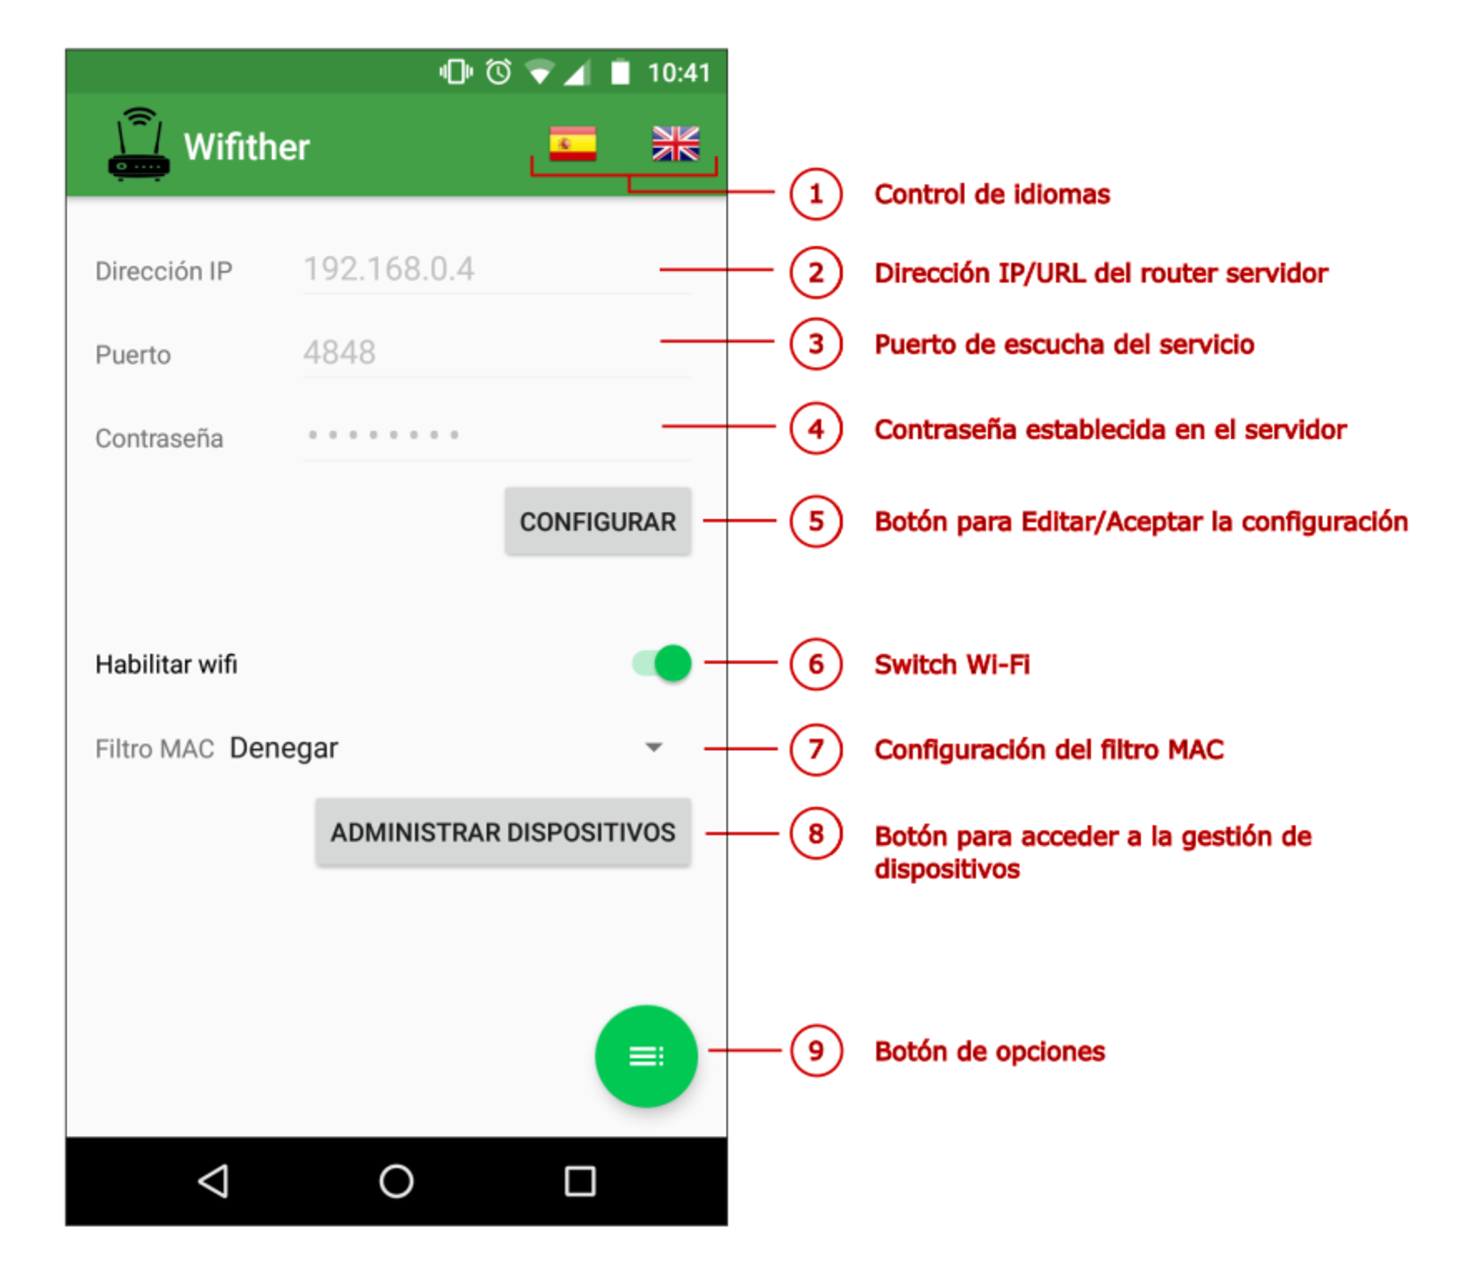
\includegraphics[scale=0.5]{main_activity_manual.eps}
                \caption{Vista principal}
                \label{fig:main_activity_manual}
        \end{figure}

        \begin{figure}[h!]
            \centering
                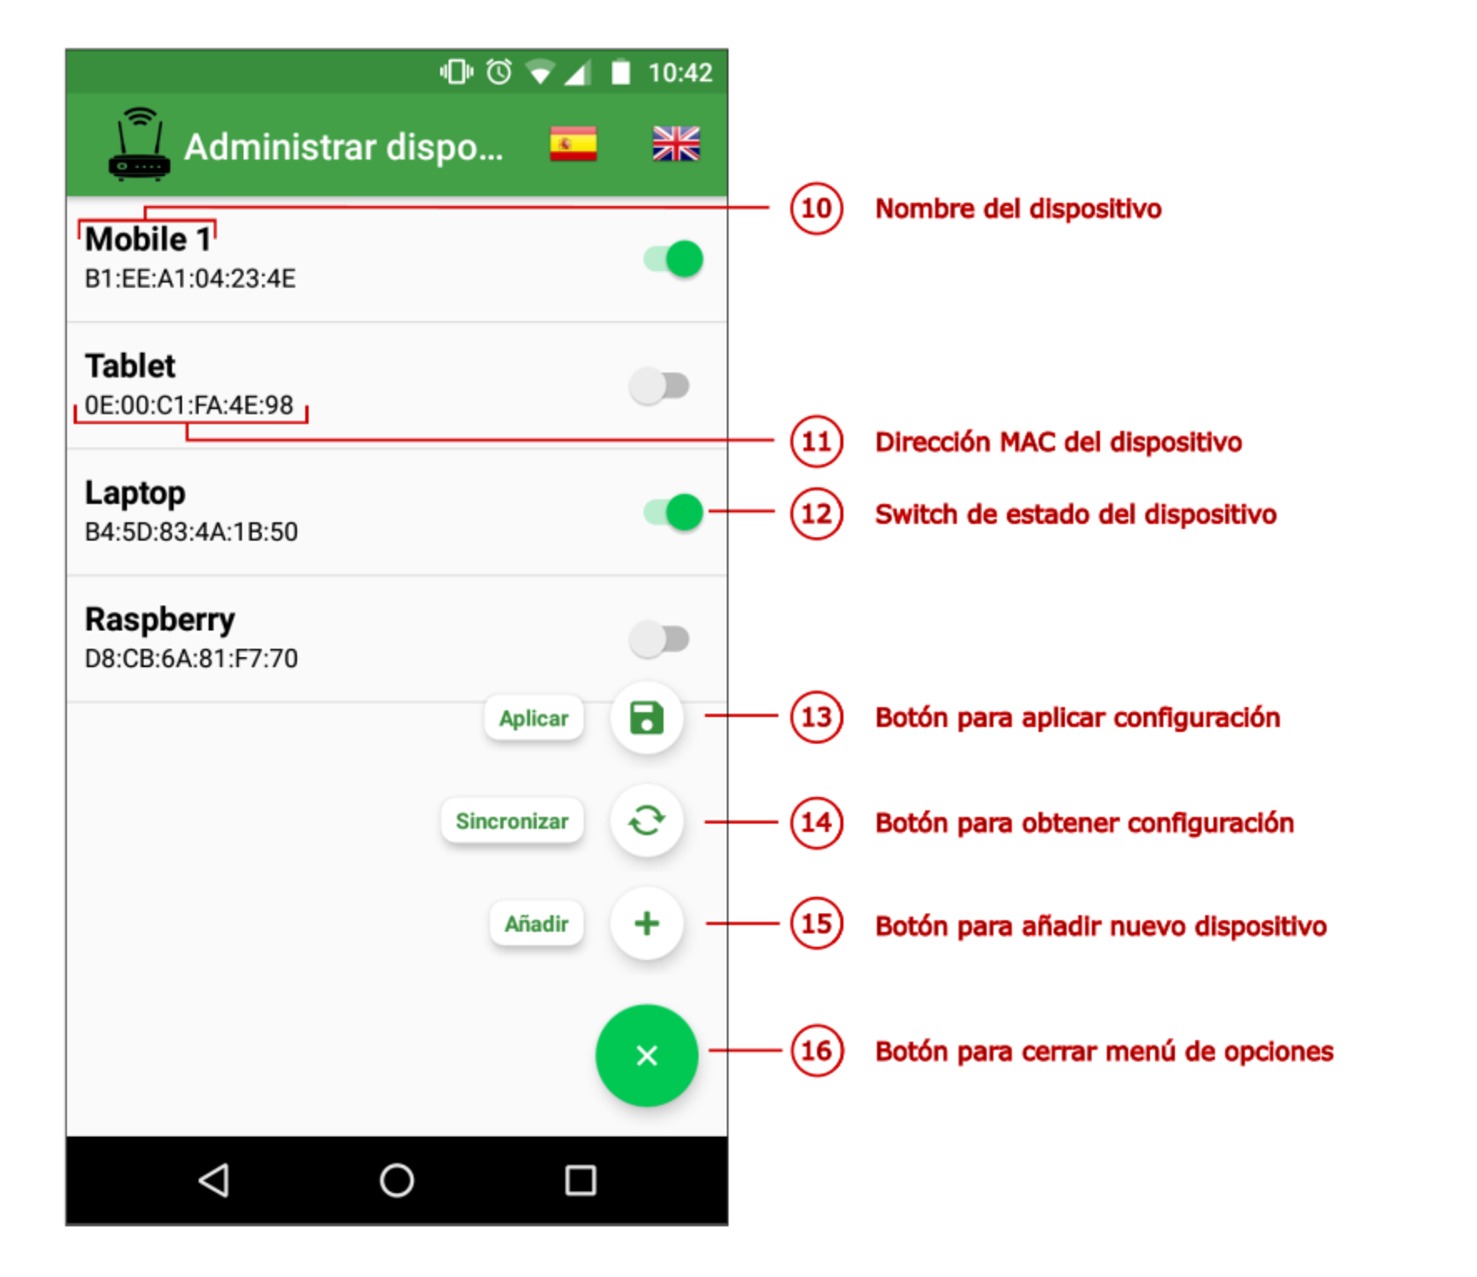
\includegraphics[scale=0.5]{devices_activity_manual.eps}
                \caption{Administración de dispositivos}
                \label{fig:devices_activity_manual}
        \end{figure}

        \begin{enumerate}

            \item \textbf{\underline{Control de idiomas}} \\
            Permite seleccionar el idioma con el que se muestran las opciones de la interfaz de usuario, están disponibles castellano e inglés, el idioma por defecto de la aplicación es el inglés.

            \item \textbf{\underline{Dirección IP/URL del router servidor}} \\
            Es el campo de texto donde se especifica la dirección del router OpenWRT en el cual se ha instalado la aplicación y sobre el que se desea gestionar la red Wi-Fi. La edición de este campo está deshabilitada por defecto, para cambiar su contenido se debe hacer uso del botón señalado con el número 5 en la \ref{fig:main_activity_manual}

            \item \textbf{\underline{Puerto de escucha del servicio}} \\
            Es el puerto que se indica al iniciar la aplicación en el router OpenWRT y que se utiliza para recibir las órdenes desde el dispositivo móvil. La edición de este campo está deshabilitada por defecto, para cambiar su contenido se debe hacer uso del botón señalado con el número 5 en la \ref{fig:main_activity_manual}

            \item \textbf{\underline{Contraseña establecida en el servidor}} \\
            Es la contraseña que se indica al iniciar la aplicación en el router OpenWRT y que se utiliza para encriptar y desencriptar las órdenes enviadas desde el dispositivo móvil. La contraseña debe contener al menos ocho caracteres. La edición de este campo está deshabilitada por defecto, para cambiar su contenido se debe hacer uso del botón señalado con el número 5 en la \ref{fig:main_activity_manual}

            \item \textbf{\underline{Botón para Editar/Aceptar la configuración}} \\
            Este botón habilita la edición de los campos de configuración señalados con los números 1, 2 y 3 en la \ref{fig:main_activity_manual}. Tras ser pulsado, el texto del botón cambia a \textit{Confirmar}, y debe ser pulsado para guardar la nueva configuración.

            \item \textbf{\underline{Switch Wi-Fi}} \\
            Enciende o apaga la red Wi-Fi en el router OpenWRT, la posición iquierda indica que la red Wi-Fi está apagada, la posición hacia la derecha indica que está encendida.

            \item \textbf{\underline{Configuración del filtro MAC}} \\
            Permite seleccionar la configuración del filtro MAC en el router OpenWRT. El selector tiene tres posiciones: \textit{Deshabilitado}, \textit{Permitir} y \textit{Denegar}.
            \begin{itemize}
                \item Si el filtro MAC está deshabilitado, cualquier dispositivo puede conectarse a la red Wi-Fi sin restricción de ningún tipo.
                \item Si el filtro MAC está configurado para \textit{Permitir}, significa que sólo pueden acceder a la red Wi-Fi los dispositivos que hayan sido especificados para que el filtro les sea aplicado.
                \item Si el filtro MAC está configurado para \textit{Denegar}, significa que tienen acceso a la red todos los dispositivos excepto los especificados para que el filtro les sea aplicado.
            \end{itemize}
            
            \item \textbf{\underline{Botón para acceder a la gestión de dispositivos}} \\
            Al pulsarlo se accede a un nuevo conjunto de opciones desde donde se pueden adicionar, editar y eliminar dispositivos, además de poder seleccionar los dispositivos con los que se desea aplicar el filtro MAC.
            \item \textbf{\underline{Botón de opciones}} \\
            Permite acceder a las opciones marcadas con los puntos 12, 14 y 15 en la \ref{fig:devices_activity_manual}
            \item \textbf{\underline{Nombre del dispositivo}} \\
            Es un indicador distintivo para cada dispositivo, es determinado por el usuario al añadir un nuevo dispositivo y es un campo obligatorio.
            \item \textbf{\underline{Dirección MAC del dispositivo}} \\
            Identificador único del adaptador de red del dispositivo. Es especificado por el usuario al añadir un nuevo dispositivo y debe cumplir con un formato específico compuesto por seis pares de caracteres hexadecimales separados por dos puntos(:). Si el formato introducido no es correcto, el botón \textit{Añadir} queda deshabilitado.
            \item \textbf{\underline{Switch de estado del dispositivo}} \\
            Añade o elimina dispositivos para que se le aplique la configuración del filtro MAC, la posición iquierda indica que la configuración del filtro \textbf{NO} se aplica al dispositivo, la posición hacia la derecha indica que la configuración del filtro \textbf{NO} se aplica al dispositivo.
            \item \textbf{\underline{Botón para aplicar configuración}} \\
            Aplica en el router OpenWRT la configuración que haya sido establecida.
            \item \textbf{\underline{Botón para optener configuración.}} \\
            Actualiza el dispositivo móvil con la configuración actual del router OpenWRT. Esta opción es útil cuando se gestiona la red desde más de un dispositivo móvil, de esta forma cada dispositivo puede saber siempre la última configuración aplicada en el router.
            \item \textbf{\underline{Botón para añadir nuevo dispositivo}} \\
            Muestra un cuadro de diálogo que permite introducir los datos del nuevo dispositivo y añadirlo a la lista de dispositivos
            \item \textbf{\underline{Botón para cerrar el menú de opciones}} \\
            Cierra el menú de opciones, también puede ser cerrado presionando sobre cualquier espacio fuera del menú.
            
        \end{enumerate}

        Para editar la información de un dispositivo, se debe mantener pulsado sobre el mismo hasta que aparezca un cuadro de diálogo y seleccionar la opción editar. La información del dispositivo debe cumplir los siguientes requisitos: El nombre de dispositivo no puede estar vacío, y la dirección MAC debe estar compuesta por seis pares de caracteres hexadecimales separados por dos puntos(:)

        Para editar la información de un dispositivo, se debe mantener pulsado sobre el mismo hasta que aparezca un cuadro de diálogo y seleccionar la opción eliminar.

        \textbf{IMPORTANTE:} Debe tenerse en cuenta que una mala configuración del filtro MAC puede provocar la pérdida de la conexión en el dispositivo desde el que se está gestionando la red Wi-Fi si está directamente conectado a esta. La configración establecida debe ser revisada cautelosamente antes de ser aplicada. En caso de pérdida de conexión por este motivo, se recomienda el restablecimiento de la conexión con el dispositivo conectado al router desde Internet en lugar de desde la red Wi-Fi.

\cleardoublepage \section{Conclusiones y trabajo futuro} \label{sec:conc}
    \subsection{Principales aportaciones}
    % deberanse destacar entre 3 e 5 aportacións importantes do
    % traballo realizado, tendo en conta os obxectivos fixados.
    Este proyecto contiene un conjunto de aportaciones a la soluciones inalámbricas disponibles actualmente en los hogares.
    
    \begin{itemize}
        \item Gestión del router a distancia
        \item Encendido y apagado de la red con la facilidad de presionar un boton
        \item Filtrado de dispositivos
        \item Mecanismos de seguridad capaces de soportar replicas de paquetes y dispositivos no autorizados
    \end{itemize}
    
    \subsection{Conclusiones}
    % incluiranse todas as conclusións de tipo técnico e persoal.
    Mantenter control del tiempo que pasan los menores en Internet es un problema que presentan todos los padres hoy en día. En este Trabajo de Fin de Grado se ha intentado facilitar esta tarea de forma que cualquier persona, sin la necesidad de conocimientos técnicos, pudiese realizarlo rápidamente. 
    
    Después de un largo proceso de desarrollo, este proyecto concluye con resultados satisfactorios, y, pese a los problemas surgidos desde sus inicios, donde la fase de investigación propuso un cambio significativo a la propuesta inicial, se considera que todos los objetivos propuestos durante su creación, han sido alcanzados. El desarrollo del proyecto ha supuesto más tiempo del planificado, pero este tiempo ha sido empleado en la creación de un sistema robusto y al alcance de cualquier hogar, brindando un mecanismo de control que no requiere de una gran inversión en infraestructira ni software especializado.

    Personalmente siento que gracias al desarrollo de este proyecto he podido afianzar y ampliar mis conocimientos en un campo que siempre ha captado mi atención y al que me gustaría dedicarme en un futuro, las redes informáticas; por lo que intentaré que no quede aquí y seguir trabajando en mi formación tanto como pueda. Durante todo el desarrollo de este proyecto he mantenido dos pautas constantes:
    
    Intentar aplicar todo lo que he aprendido durante estos últimos cuatro años, y unas palabras que me dijo mi tutor al comenzar a trabajar juntos: ``Haz un proyecto del que te sientas orgulloso...''. En estos momentos, creo que lo he conseguido.

    \subsection{Trabajo futuro}
    % presentaranse posible ampliacións e traballos relacionados por facer.
        \subsubsection{Gestión de horarios}
        Dado que todos los seres humanos normalmente seguimos rutinas, incuídos los menores, sería interesante crear un macanismo que permita planificar los horarios en los que cierto dispositivo tiene acceso a Internet. Esta es una forma simple de evitar problemas por olvidos y facilitar la gestión diaria de la conectividad en el hogar.

        \subsubsection{Cuotas de navegación}
        Aunque la educación por recompensa conlleve sus desventajas, está claro que siempre incita al esfuerzo. Por ello, una posible ampliación sería un sistema que permita configurar cuotas de navegación para los dispositivos en función de las notas obtenidas desde una secretaría virtual.

        Esto requeriría un estudio de viabilidad, teniendo en cuenta que no todos los colegios disponen de secretarías virtuales para la entrega de notas, ni todas las secretarías virtuales poseen las mismas características.

        \subsubsection{Integración de OpenVPN}
        La solución planteada en este proyecto incluye el uso de un túnel utilizando la aplicación móvil OpenVPN for Android como mecanismo de seguridad para evitar que los paquetes enviados desde el dispositivo cliente puedan ser replicados. Una mejora a este sistema sería integrar OpenVPN como una opción dentro de la propia aplicación móvil desarrollada, brindando más facilidad de configuración y evitando la instalación de aplicaciones de terceros.

        \subsubsection{Filtrado de MACS para dispositivos clientes}
        Implementar un filtro que permita identificar los clientes autorizados a modificar la configuración del router sería una buena medida de seguridad adicional que no pudo ser implementada durante el desarrollo del proyecto debido a los retrasos que provocaría.

        \subsubsection{Aplicación iOS}
        Dado que el número de dispositivos iOS aumenta cada año, es una buena idea portar el código de la aplicación Android desarrollada para que esté disponible en este sistema operativo.

\bibliographystyle{plain}
\bibliography{biblio}

% deberanse citar todas as fontes de información empregadas para a realización do traballo.

% 1. Autor/a/es/as.

% 2. Título do artigo, libro, monografía,...

% 3. Editorial ou nome da revista.

% 4. Número da revista, volume e páxinas (só para revistas).

% 5. Ano de publicación.

% 6. Dirección e data de consulta (só para URL).

% Recoméndase empregar para referencias de artigos, revistas, e outras fontes de

% referencia, o formato APA, ISO 690, IEEE ou similares, e uniformizados ao longo de

% toda a sección.

% Deberase empregar un estilo uniforme para todas elas e aportarase, en cada caso:

\cleardoublepage \section{Anexos} \label{anx:dependences}
    \appendix
    \section{Tabla de dependencias del SDK}
    \begin{table}[h!]             
        \centering                  
            \resizebox{\textwidth}{!}{   
                \begin{tabular}{|l|l|l|}
                    \hline
                    \textbf{Prerequisitos}  & \textbf{Debian}   & \textbf{Arch}             \\           
                    \hline
                    asciidoc                & asciidoc          & asciidoc                  \\
                    GNU Bash                & bash              & bash                      \\
                    GNU bc                  & bc                & bc                        \\
                    GNU Binutils            & binutils          & binutils                  \\
                    bzip2                   & bzip2             & bzip2                     \\
                    fastjar                 & fastjar           & fastjar                   \\
                    flex                    & flex              & flex                      \\
                    git                     & git-core          & git                       \\
                    GNU C Compiler          & gcc               & gcc                       \\
                    getopt                  & util-linux        & util-linux                \\
                    GNU awk                 & gawk              & gawk                      \\
                    libz, libz-dev          & zlib1g-dev        & zlib                      \\
                    Mercurial / hg          &                   & mercurial                 \\
                    make                    & make              & make                      \\
                    mkisofs                 & genisoimage       & cdrkit                    \\
                    ncurses                 & libncurses5-dev   & ncurses                   \\
                    openssl/ssl.h           & libssl-dev        & openssl                   \\
                    patch                   & patch             & patch                     \\
                    perl-ExtUtils-MakeMaker & perl-modules      & perl-extutils-makemaker   \\
                    python2.6-dev           & python2.6-dev     & python2                   \\
                    rsync                   & rsync             & rsync                     \\
                    ruby                    & ruby              & ruby                      \\
                    sdcc                    & sdcc              & sdcc                      \\
                    subversion              & subversion        & subversion                \\
                    unzip                   & unzip             & unzip                     \\
                    GNU Wget                & wget              & wget                      \\
                    xgettext                & gettext           & gettext                   \\
                    xsltproc                & xsltproc          & libxslt                   \\
                    zlib, zlib-static       & zlib1g-dev        & zlib                      \\
                    \hline
                \end{tabular}
            }
        \caption{Dependencias del SDK}
        \label{tab:sdk_dependences}
    \end{table}

    \section{Detalles de la planificación}
    \begin{table}[h!]             
        \centering                  
            \resizebox{\textwidth}{!}{   
                \begin{tabular}{|l|l|l|}
                    \hline
                    \textbf{Prueba realizada}  & \textbf{Resultado esperado}   & \textbf{Resultado de la prueba}             \\           
                    \hline
                    Envío de paquete a una servidor no existente & Fallo          & Éxito                  \\
                    Envío de un paquete al servidor correcto sin ejecutar el servicio    & Fallo              & Éxito                      \\
                    Envío de un paquete sin contenido de control                  & Fallo                & Éxito                        \\
                    Envío de un paquete válido            & Éxito          & Éxito                  \\
                    \hline
                \end{tabular}
            }
        \caption{Pruebas de conectividad}
        \label{tab:conectivity_tests}
    \end{table}

    \begin{table}[h!]             
        \centering                  
            \resizebox{\textwidth}{!}{   
                \begin{tabular}{|l|l|l|}
                    \hline
                    \textbf{Prueba realizada}  & \textbf{Resultado esperado}   & \textbf{Resultado de la prueba}             \\           
                    \hline
                    Campo IP vacío                & Fallo          & Éxito                  \\
                    Campo puerto vacío                & Fallo          & Éxito                  \\
                    Campo contraseña vacío                & Fallo          & Éxito                  \\
                    Campo contraseña conn menos de 8 dígitos                & Fallo          & Éxito                  \\
                    Campo IP con una dirección incorrecta                & Fallo          & Éxito                  \\
                    Campo puerto con un valor incorrecto                & Fallo          & Éxito                  \\
                    Campos con datos correctos                & Éxito          & Éxito                  \\
                    \hline
                \end{tabular}
            }
        \caption{Pruebas de entrada}
        \label{tab:input_tests}
    \end{table}

        \begin{table}[h!]             
        \centering                  
            \resizebox{\textwidth}{!}{   
                \begin{tabular}{|l|l|l|}
                    \hline
                    \textbf{Prueba realizada}  & \textbf{Resultado esperado}   & \textbf{Resultado de la prueba}             \\           
                    \hline
                    Campo contraseña vacío en el cliente               & Fallo          & Éxito                  \\
                    Campo contraseña vacío en el servidor               & Fallo          & Éxito                  \\
                    Campo contraseña conn menos de 8 dígitos en el cliente               & Fallo          & Éxito                  \\
                    Campo contraseña conn menos de 8 dígitos en el servidor               & Fallo          & Éxito                  \\
                    Comparaciones realizadas durante el desarrollo con la librería OpenSSL                & Exito          & Éxito                  \\
                    Campo contraseña con el mismo valor correcto en cliente y servidor                & Éxito          & Éxito                  \\
                    \hline
                \end{tabular}
            }
        \caption{Pruebas de encriptación}
        \label{tab:cripto_tests}
    \end{table}

    \subsubsection{Descripción de las fases}
        La fase de investigación tiene como propósito analizar las necesidades a solventar en cuanto al control de redes Wi-Fi en los hogares, y con ellas determinar las características que debe tener el sistema que va a ser creado. Esta fase incluye el análisis de los routers actuales y la realización de una comparativa entre las soluciones aportadas por los diferentes proveedores de Internet. Las tareas relacionadas con esta fase se pueden encontrar en la tabla \ref{tab:fases_inv}.

        
        \begin{table}[h!]
            \centering
                \resizebox{\textwidth}{!}{
                    \begin{tabular}{|l|c|}
                        \hline
                        \textbf{Tarea}                                                              &   \textbf{Estimación temporal} (Días) \\           
                        \hline
                        Investigación acerca de las necesidades de control en redes Wi-Fi           &   0.5                                 \\
                        Análisis de routers actuales                                                &   0.5                                 \\
                        Comparativa de las soluciones aportadas por los proveedores de Internte     &   0.5                                 \\
                        Análisis de las características del sistema a desarrollar                   &   0.5                                 \\
                        \hline
                    \end{tabular}
                }
            \caption{Descripción de la fase de investigación}
            \label{tab:fases_inv}
        \end{table}

        \paragraph{ Boceto}
        En esta fase se realiza un estudio de los objetivos generales del sistema que se desarrolla, cada uno de ellos es analizado para definir sus características fundamentales. Con los resultados obtenidos se realiza el diseño de la arquitectura que será utilizado, definiendo el sistema, los subsistemas que lo componen, y las estrategias a utilizar para su construcción. Las tareas necesarias para el desarrollo de esta fase se encuentran el la tabla \ref{tab:fases_boc}.

        \begin{table}[h!]             
            \centering                  
                \resizebox{\textwidth}{!}{   
                    \begin{tabular}{|l|c|}
                        \hline
                        \textbf{Tarea}                                                              &   \textbf{Estimación temporal} (Días) \\           
                        \hline
                        Análisis de los objetivos generales del sistema                             &   0.25                                \\
                        Análisis detallado de los subobjetivos                                      &   0.25                                \\
                        Diseño de la arquitectura del sistema                                       &   1                                   \\
                        Planificación de los sprints de desarrollo                                  &   0.5                                 \\
                        \hline
                    \end{tabular}
                }
            \caption{Descripción de la face Boceto}
            \label{tab:fases_boc}
        \end{table}
        
        \paragraph{ Compilación cruzada}
        En esta fase se busca abarcar toda la documentación posible acerca de la compilación cruzada desde distribuciones GNU/Linux para OpenWRT. Se compila un paquete ``Hola mundo'' utilizando tanto el \textit{Toolchain} como el \textit{SDK} proporcionado por OpenWRT \cite{SDK} y se comprueba su funcionamiento en el router donde se realizarán las pruebas de desarrollo del sistema en cada uno de los sprints. En la tabla \ref{tab:fases_cc} pueden encontrarse las tareas que incluye esta fase.

        \begin{table}[h!]             
            \centering                  
                \resizebox{\textwidth}{!}{                      
                    \begin{tabular}{|l|c|}
                        \hline
                        \textbf{Tarea}                                                              &   \textbf{Estimación temporal} (Días) \\           
                        \hline
                        Desarrollo de un sistema de prueba                                          &   0.2                                 \\
                        Compilación utilizando el toolchain de OpenWRT                              &   1                                   \\
                        Compilación utilizando el SDK de OpenWRT                                    &   2                                   \\
                        Realización de pruebas de funcionamiento en el router                       &   0.8                                 \\
                        \hline
                    \end{tabular}
                }
            \caption{Descripción de la fase de compilación cruzada}
            \label{tab:fases_cc}
        \end{table}

        \paragraph{ Sprint 1: Implementación de la aplicación Android base}
        En el primer sprint se busca crear una aplicación sencilla para dispositivos Android. Debe tener una interfaz básica, con las opciones necesarias para la configuración del servidor resultante del \textit{Sprint 2}. También debe implementar la gestión de paquetes UDP, se envian paquetes de control y se reciben paquetes de confirmación y paquetes de actualización de estado. Las tareas de esta fase se encuentran en la tabla \ref{tab:fases_sp1}.

        \begin{table}[h!]             
            \centering                  
                \resizebox{\textwidth}{!}{   
                    \begin{tabular}{|l|c|}
                        \hline
                        \textbf{Tarea}                                                              &   \textbf{Estimación temporal} (Días) \\           
                        \hline
                        Diseño de pruebas                                                           &   0.5                                 \\
                        Implementar interfaz base                                                   &   0.2                                 \\
                        Implementar configuraciones Android                                         &   0.2                                 \\
                        Implementar cliente                                                         &   0.6                                 \\
                        Implementar servidor de confirmación                                        &   2                                   \\
                        Implementar servidor de actualización                                       &   2                                   \\
                        Validación de pruebas y corrección de errores                               &   0.5                                 \\
                        \hline
                    \end{tabular}
                }
            \caption{Descripción del sprint 1}
            \label{tab:fases_sp1}
        \end{table}

        \paragraph{ Sprint 2: Implementación del servidor}
        El objetivo del segundo sprint es desarrollar el sistema servidor, éste debe contener un socket que le permita recibir peticiones y responder a éstas \cite{Socket}. También debe modificar las configuraaciones necesarias de acuerdo al mensaje de control recibido desde el cliente, y debe poder ser ejecutado como un servicio demonio, no deberá bloquear la terminal ni terminar su ejecución cuando la sesión desde la que ha sido iniciado sea finalizada. La tabla \ref{tab:fases_sp2} muestra las tareas de esta fase.

        \begin{table}[h!]             
            \centering                  
                \resizebox{\textwidth}{!}{   
                    \begin{tabular}{|l|c|}
                        \hline
                        \textbf{Tarea}                                                              &   \textbf{Estimación temporal} (Días) \\           
                        \hline
                        Diseño de pruebas                                                           &   0.5                                 \\
                        Implementación del socket                                                   &   2                                   \\
                        Implementación de funcionalidades                                           &   2                                   \\
                        Demonizar                                                                   &   1                                   \\
                        Validación de pruebas y corrección de errores                               &   0.5                                 \\
                        \hline
                    \end{tabular}
                }
            \caption{Descripción del sprint 2}
            \label{tab:fases_sp2}
        \end{table}

        \paragraph{ Sprint 3: Implementación de sistemas de seguridad}
        En el tercer sprint se procede con el desarrollo de los sistemas de seguridad planteados durante el análisis. Se implementan los métodos de encriptación \textit{DES} para los mensajes de control que son enviados al servidor, y el resultado de estos métodos, a su vez, es encriptado en \textit{Base64}, de forma que pueda ser enviado mediante datagramas. También se implementan los mecanismos de desencriptación tanto \textit{Base64} como \textit{DES} que son utilizados en el servidor tras recibir los paquetes UDP enviados desde el cliente. Las tareas relacionadas con esta fase pueden ser encontradas en la tabla \ref{tab:fases_sp3}.

        \begin{table}[h!]             
            \centering                  
                \resizebox{\textwidth}{!}{   
                    \begin{tabular}{|l|c|}
                        \hline
                        \textbf{Tarea}                                                              &   \textbf{Estimación temporal} (Días) \\           
                        \hline
                        Encriptación DES en cliente                                                 &   0.5                                 \\
                        Encriptación Base64 en cliente                                              &   0.5                                 \\
                        Decriptación Base64 en servidor                                             &   2                                   \\
                        Decriptación DES en servidor                                                &   0.5                                 \\
                        \hline
                    \end{tabular}
                }
            \caption{Descripción del sprint 3}
            \label{tab:fases_sp3}
        \end{table}

        \paragraph{ Sprint 4: Implementación de la interfaz gráfica de la aplicación}
        Durante el cuarto sprint se implementa la interfaz gráfica final de la aplicación Android. Debe disponer de una actividad principal con opciones de configuración, y una actividad para la gestión de dispositivos, donde estos puedan ser almacenados en una lista. Esta lista, mediante un adaptador \cite{ArrayAdapter}, debe permitir la visualización de los datos de cada dispositivo y su controlador de configuración. Es importante que el sistema esté disponible en múltiples idiomas. La tabla \ref{tab:fases_sp4} indica las tareas relacionadas con esta fase.

        \begin{table}[h!]             
            \centering                  
                \resizebox{\textwidth}{!}{   
                    \begin{tabular}{|l|c|}
                        \hline
                        \textbf{Tarea}                                                              &   \textbf{Estimación temporal} (Días) \\           
                        \hline
                        Diseño de pruebas unitarias                                                 &   0.5                                 \\
                        Desarrollo de la actividad principal                                        &   0.2                                 \\
                        Modelo de dispositivos personalizados                                       &   0.2                                 \\
                        Adaptador de dispositivos personalizado                                     &   0.6                                 \\
                        Desarrollo de diálogos y menús                                              &   2                                   \\
                        Implementación de la gestión de idiomas                                     &   2                                   \\
                        Validación de pruebas y corrección de errores                               &   0.5                                 \\
                        \hline
                    \end{tabular}
                }
            \caption{Descripción del sprint 4}
            \label{tab:fases_sp4}
        \end{table}

        \paragraph{ Sprint 5: Integración de sistemas}
        El resultado del cuarto sprint debe ser el proyecto totalmente integrado, inculyendo los resultados de los sprints anteriores, proporcionando así un sistema sólido, sin errores y listo para ser explotado. Las tareas correspondientes a esta fase pueden encontrarse en la tabla \ref{tab:fase_sp5}.

        \begin{table}[h!]             
            \centering                  
                \resizebox{\textwidth}{!}{   
                    \begin{tabular}{|l|c|}
                        \hline
                        \textbf{Tarea}                                                              &   \textbf{Estimación temporal} (Días) \\           
                        \hline
                        Integración de la interfaz gráfica y los sistemas de conexión               &   3                                   \\
                        Integración de los sistemas de seguridad                                    &   2                                   \\
                        Validación de pruebas y corrección de errores                               &   0.5                                 \\
                        \hline
                \end{tabular}
                }
            \caption{Descripción del sprint 5}
            \label{tab:fase_sp5}
        \end{table}

        \paragraph{ Documentación}
        La documentación es un proceso que abarca el desarrollo de todo el proyecto salvo la fase de investigación inicial, donde no están clarificadas las bases del sistema a desarrollar. Documentar incluye tanto la memoria de proyecto, como la fase de cierre donde se completa con los manuales y guías para el usuario. Además, se debe tener en cuenta que mantener un código correctamente ordenado y comentado también es parte de la documentación. Las tareas de ésta fase pueden ser consultadas en la tabla \ref{tab:fase_doc}.

        \begin{table}[h!]             
            \centering                  
                \resizebox{\textwidth}{!}{   
                    \begin{tabular}{|l|c|}
                        \hline
                        \textbf{Tarea}                                                              &   \textbf{Estimación temporal} (Días) \\         
                        \hline
                        Elaboración de la memoria                                                   &   38                                  \\
                        Cierre                                                                      &   2                                   \\
                        \hline
                    \end{tabular}
                }
            \caption{Descripción de la fase de documentación}
            \label{tab:fase_doc}
        \end{table}
% incluiranse outros elementos de interese no TFG que se consideren necesarios para a

% mellor comprensión do mesmo.



\end{document}
